%%%%%%%%%%%%%%%%%%%%%%%%%%%%%%%%%%%%%%%%%
% Journal Article
% LaTeX Template
% Version 1.3 (9/9/13)
%
% This template has been downloaded from:
% http://www.LaTeXTemplates.com
%
% Original author:
% Frits Wenneker (http://www.howtotex.com)
%
% License:
% CC BY-NC-SA 3.0 (http://creativecommons.org/licenses/by-nc-sa/3.0/)
%
%%%%%%%%%%%%%%%%%%%%%%%%%%%%%%%%%%%%%%%%%

%----------------------------------------------------------------------------------------
%	PACKAGES AND OTHER DOCUMENT CONFIGURATIONS
%----------------------------------------------------------------------------------------

\documentclass[oneside]{article}

\usepackage{lipsum} % Package to generate dummy text throughout this template
\usepackage{amsmath}
\usepackage[sc]{mathpazo} % Use the Palatino font
\usepackage[T1]{fontenc} % Use 8-bit encoding that has 256 glyphs
\linespread{1.05} % Line spacing - Palatino needs more space between lines
\usepackage{microtype} % Slightly tweak font spacing for aesthetics
\usepackage{amsmath}

\usepackage[hmarginratio=1:1,top=32mm,columnsep=20pt]{geometry} % Document margins
\usepackage{multicol} % Used for the two-column layout of the document
\usepackage[hang, small,labelfont=bf,up,textfont=it,up]{caption} % Custom captions under/above floats in tables or figures
\usepackage{booktabs} % Horizontal rules in tables
\usepackage{float} % Required for tables and figures in the multi-column environment - they need to be placed in specific locations with the [H] (e.g. \begin{table}[H])
\usepackage{hyperref} % For hyperlinks in the PDF
\restylefloat{figure}
\usepackage{graphicx}
\usepackage{array}
\newcolumntype{C}[1]{>{\centering\arraybackslash}p{#1}}

\usepackage{lettrine} % The lettrine is the first enlarged letter at the beginning of the text
\usepackage{paralist} % Used for the compactitem environment which makes bullet points with less space between them

\usepackage{abstract} % Allows abstract customization
\renewcommand{\abstractnamefont}{\normalfont\bfseries} % Set the "Abstract" text to bold
%\renewcommand{\abstracttextfont}{\normalfont\small\itshape} % Set the abstract itself to small italic text

\usepackage{titlesec} % Allows customization of titles
%\renewcommand\thesection{\Roman{section}} % Roman numerals for the sections
%\renewcommand\thesubsection{\Roman{subsection}} % Roman numerals for subsections
%\titleformat{\section}[block]{\large\scshape\centering}{\thesection.}{1em}{} % Change the look of the section titles
\titleformat{\subsection}[block]{\large}{\thesubsection.}{1em}{} % Change the look of the section titles

\usepackage{fancyhdr} % Headers and footers
\pagestyle{fancy} % All pages have headers and footers
\fancyhead{} % Blank out the default header
\fancyfoot{} % Blank out the default footer
%\fancyhead[C]{Hall C Collaboration $\bullet$ \today} % Custom header text
\fancyhead[C]{\today} % Custom header text
\fancyfoot[RO,LE]{\thepage} % Custom footer text
\usepackage{authblk}

%----------------------------------------------------------------------------------------
%	TITLE SECTION
%----------------------------------------------------------------------------------------

\title{\vspace{-15mm}\fontsize{20pt}{10pt}\selectfont\textbf{A new method to study the EMC Effect using the $F_2^{n}$ structure function}} % Article title

\author[1]{H. Szumila-Vance}
\author[2]{I. Cloet}
\author[1]{C. Keppel}
\author[3]{S. Escalante}
\author[3]{N. Kalantarians}
\affil[1]{Thomas Jefferson National Accelerator Facility, Newport News, VA}
\affil[2]{Argonne National Laboratory, Argonne, IL}
\affil[3]{Virginia Union University, Richmond, VA}
\renewcommand\Authands{ , }



%\author{
%\large
%\textsc{Holly Szumila-Vance}\thanks{}\\[2mm] % Your name
%\normalsize Jefferson Lab \\ % Your institution
%\normalsize \href{mailto:hszumila@jlab.org}{hszumila@jlab.org} % Your email address
%\vspace{-5mm}
%}
\date{}

%----------------------------------------------------------------------------------------

\begin{document}

\maketitle % Insert title

\thispagestyle{fancy} % All pages have headers and footers

%----------------------------------------------------------------------------------------
%	ABSTRACT
%----------------------------------------------------------------------------------------

\begin{abstract}
The persistently mysterious deviations from unity of the ratio of nuclear target structure functions to those of deuterium as measured in deep inelastic scattering (termed the ``EMC Effect") have become the canonical observable for studies of nuclear medium modifications to free nucleon structure in the valence regime. The structure function of the free proton is well known from numerous experiments spanning decades. The free neutron structure function, however, has remained difficult to access. Only recently has it been extracted in a systematic study of the global data within a parton distribution function extraction framework and is available from the CTEQ-Jefferson Lab (CJ) Collaboration. Here we leverage the latter to introduce a new method to study the EMC Effect in nuclei by re-examining existing data and by now determining the magnitude of the medium modifications to the free neutron and proton structure functions independently. From the extraction of the free neutron from world data, it is possible to examine the nuclear effects in deuterium and their contribution to our interpretation of the EMC Effect. In this study, we observe that the ratio of the deuteron to the sum of the free neutron and proton structure functions has some $x_{B}$ and $Q^{2}$ dependencies implying that the magnitude of the standard EMC Effect is in part due to the nuclear effects of the deuteron and also exhibits some $x_{B}$ and $Q^{2}$ dependence.
\end{abstract}
%\newpage
%\tableofcontents
%\newpage
 %\listoffigures
% \newpage
%\listoftables
%\newpage
%----------------------------------------------------------------------------------------
%	ARTICLE CONTENTS
%----------------------------------------------------------------------------------------


\section{Introduction}

The EMC Effect



We chose to use the SLAC E139 data set because it is the most complete published list of cross sections available. From the initial cross sections given, we converted the absolute cross section to the structure function by using the kinematics and R1990 fitting. 


\begin{figure}[H]
  \centering
      	  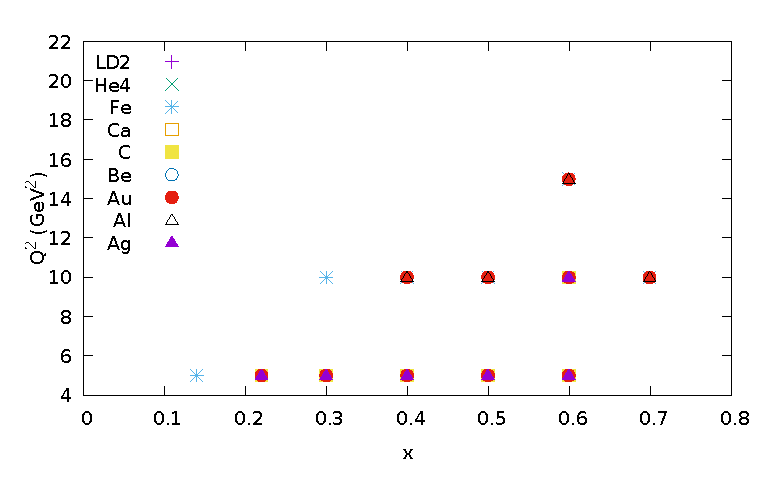
\includegraphics[width=0.5\textwidth]{plots/F2ADdataQ2vsx.eps}
 	 \caption[]{}
  \label{fig:slac_q2x}
 \end{figure} 
 
\section{Theory predictions using nuclear matter}

Discussion points: predicted d/n and d/p ratios, interpretations in quark distributions, emc effects in deuterium


  
\begin{figure}[H]
  \centering
      	  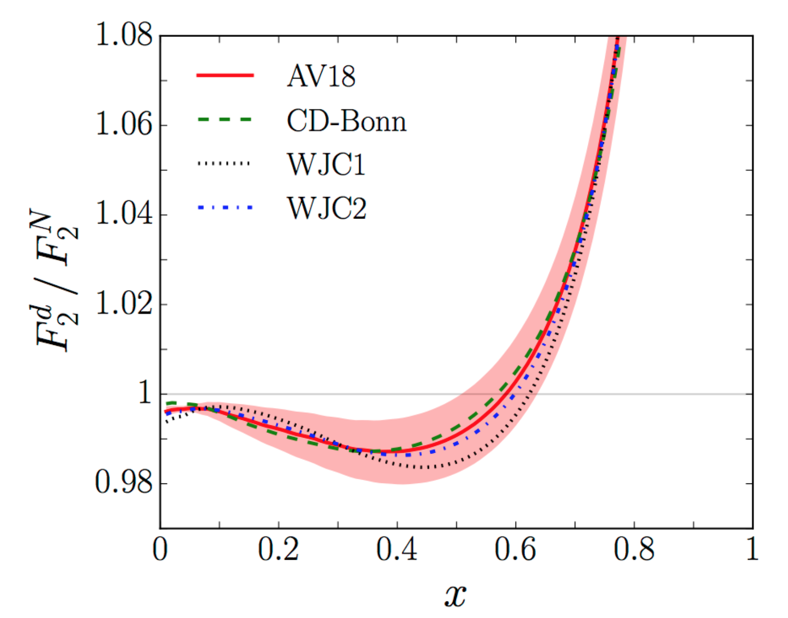
\includegraphics[width=0.5\textwidth]{plots/dn_effects_theory.png}
 	 \caption[Theoretical extraction of the ratio of $F_2^d/F_2^N$]{The theoretical extraction of the ratio of $F_2^d/F_2^N$. The deuteron exhibits some $x_B$-dependence such that the ratio is modified by approximately 2$\%$ in the regime of $x_B$ between 0.3--0.7 (region of interest to the EMC Effect).}
  \label{fig:dn_theory}
 \end{figure}  
 
\begin{figure}[H]
  \centering
      	  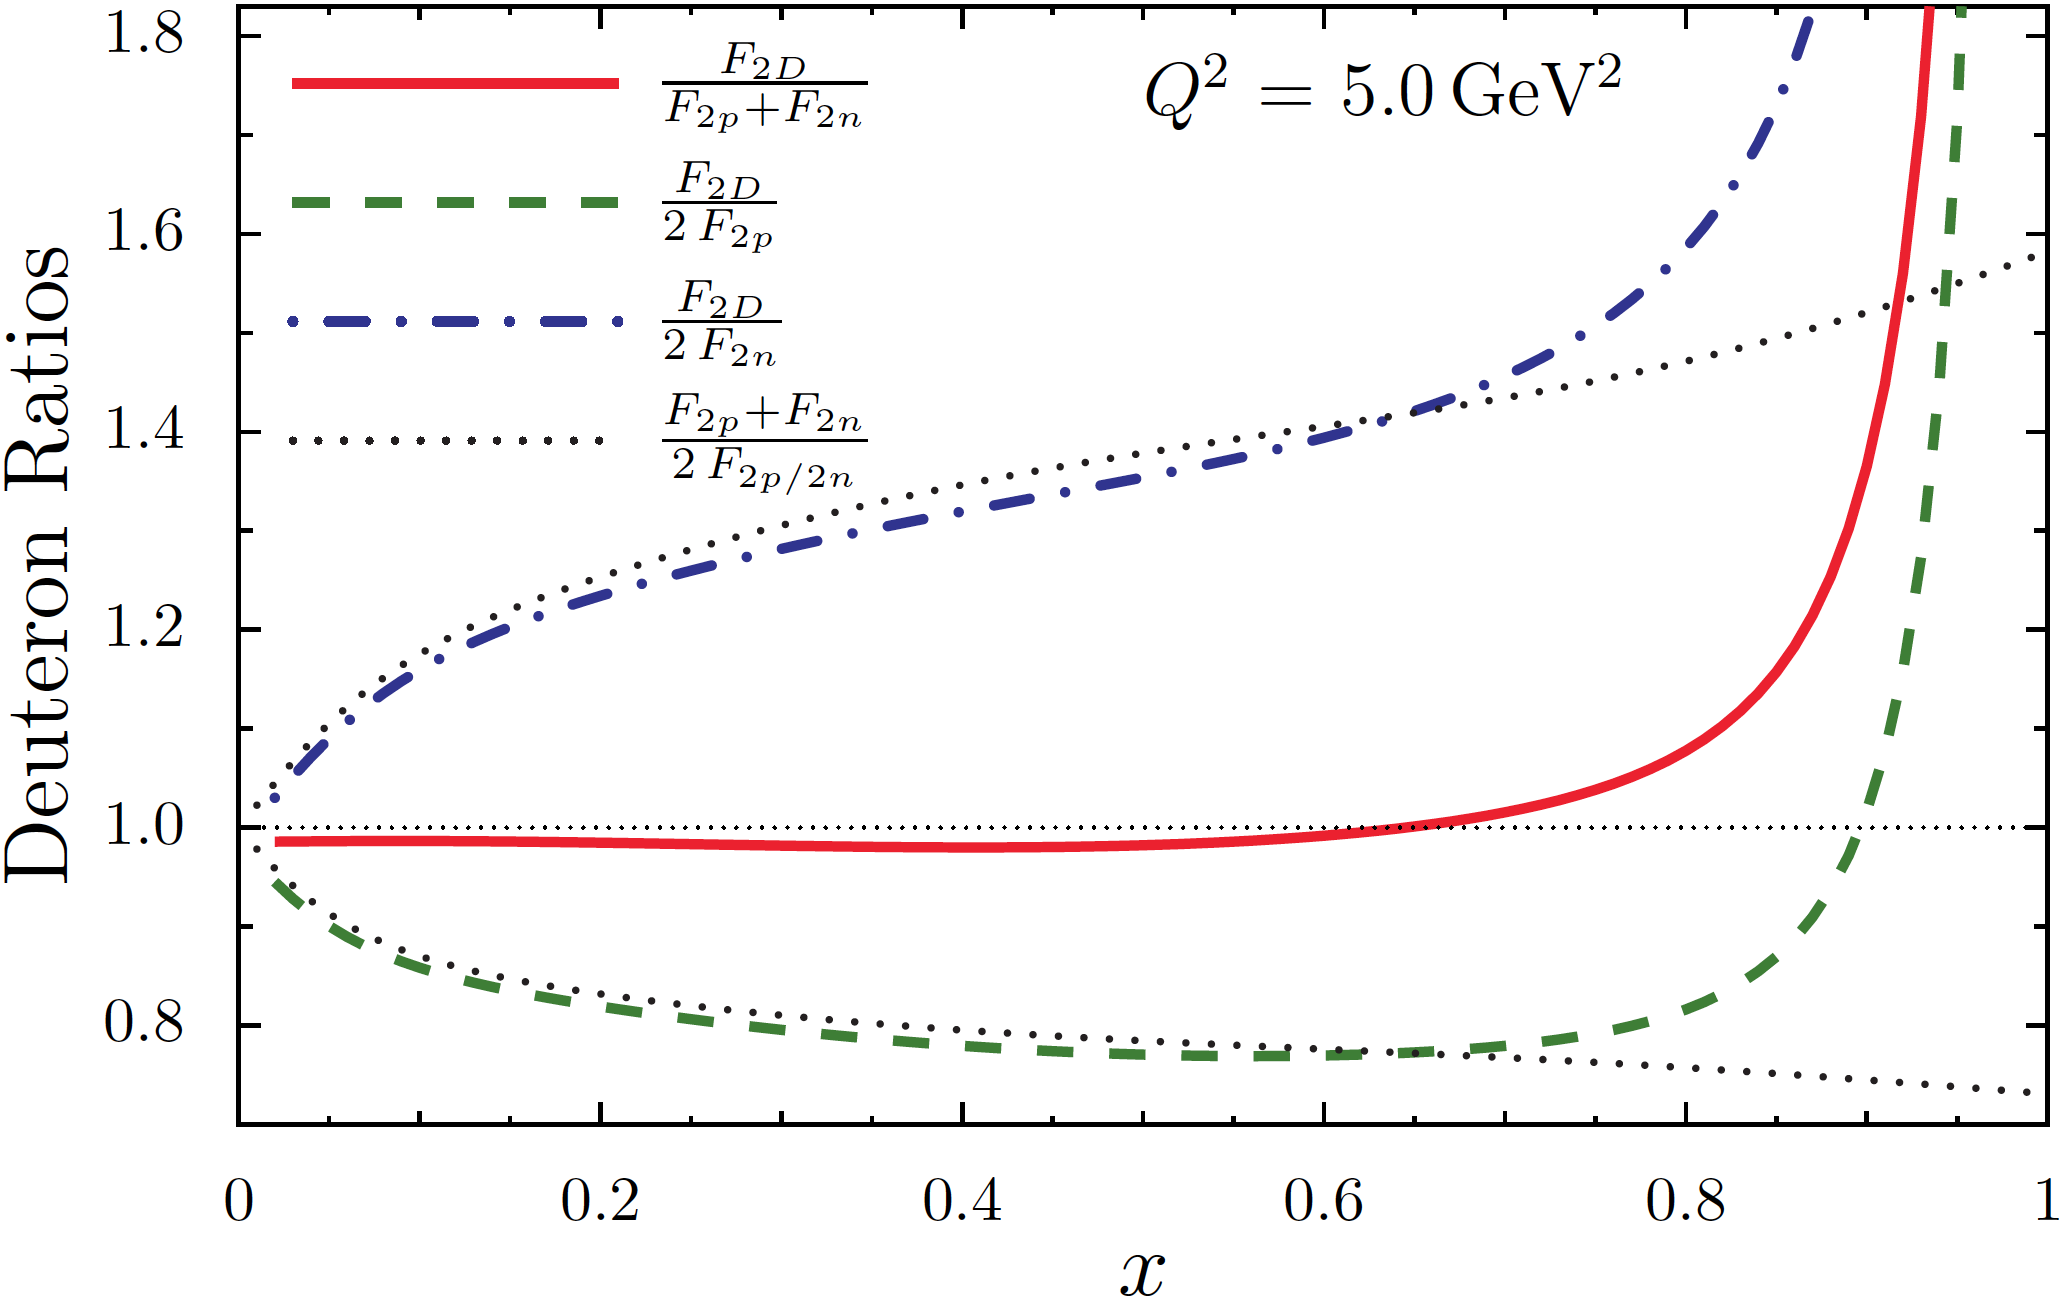
\includegraphics[width=0.5\textwidth]{plots/deut_ratio_theory.png}
 	 \caption[Theoretically-derived deuteron $F_2$ ratios with respect to the free nucleons]{Theoretically-derived deuteron $F_2$ ratios with respect to the free neutron and proton, the free proton, and the free neutron are shown for $Q^2=5$.}
  \label{fig:deut_theory}
 \end{figure}  
  
\section{$F_2^n$ extraction and the CJ15 fit}

We need to point to CJ and how the world data was extracted. 

 \begin{figure}
\begin{minipage}{0.5\textwidth}
 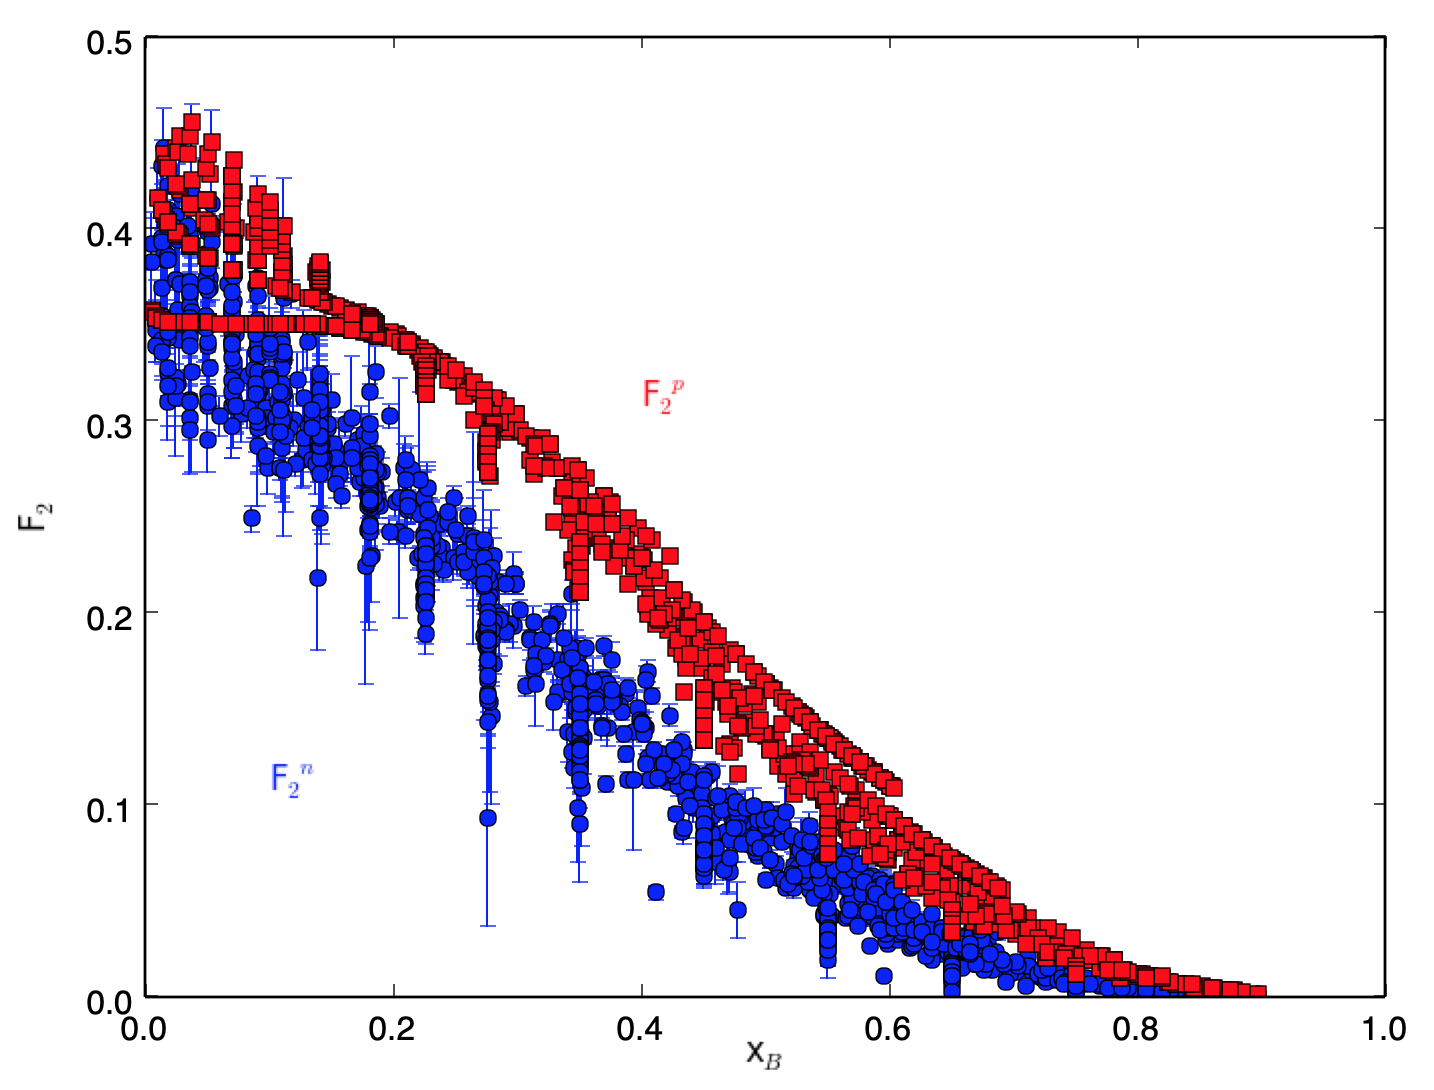
\includegraphics[width=\textwidth]{plots/f2np_plot.png}
\end{minipage}\hfill\begin{minipage}{0.5\textwidth}
 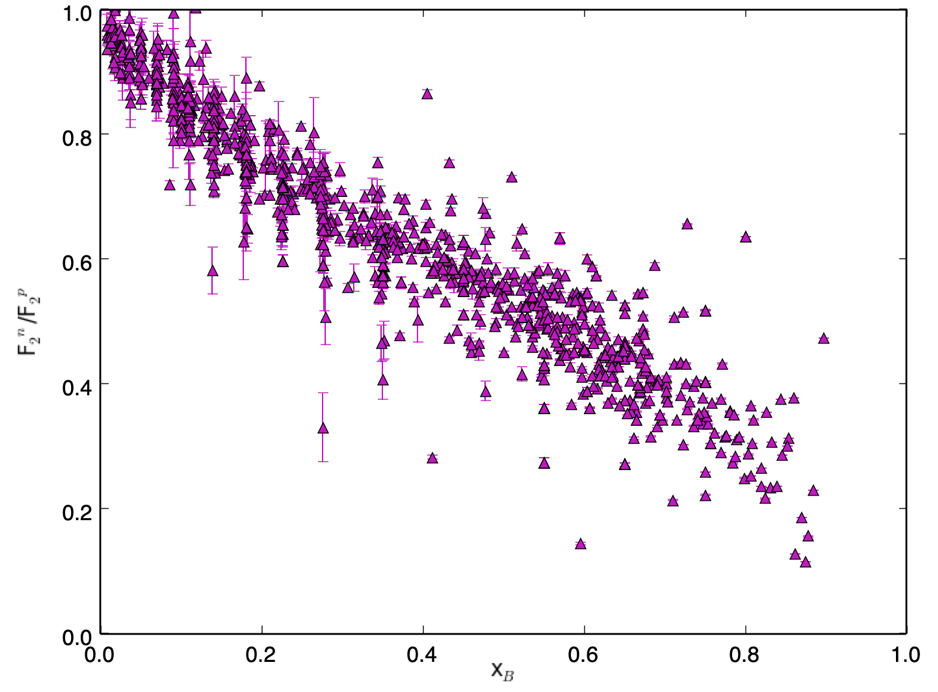
\includegraphics[width=\textwidth]{plots/f2npratio_plot.png}
 \end{minipage}
  \caption[$F_2^{n,p}$ characteristics]{Left: The extracted $F_2^n$ from the world DIS data is shown in blue, and the $F_2^p$ from the NMC global fit is shown in red for the same corresponding $x_B$ and $Q^2$. Right: The ratio of the $F_2^n/F_2^p$ from the left is shown as a function of $x_B$.}
  \label{fig:F2np_general}
\end{figure} 
 
\subsection{$Q^2$ dependence}

\begin{figure}
\begin{minipage}{0.5\textwidth}
 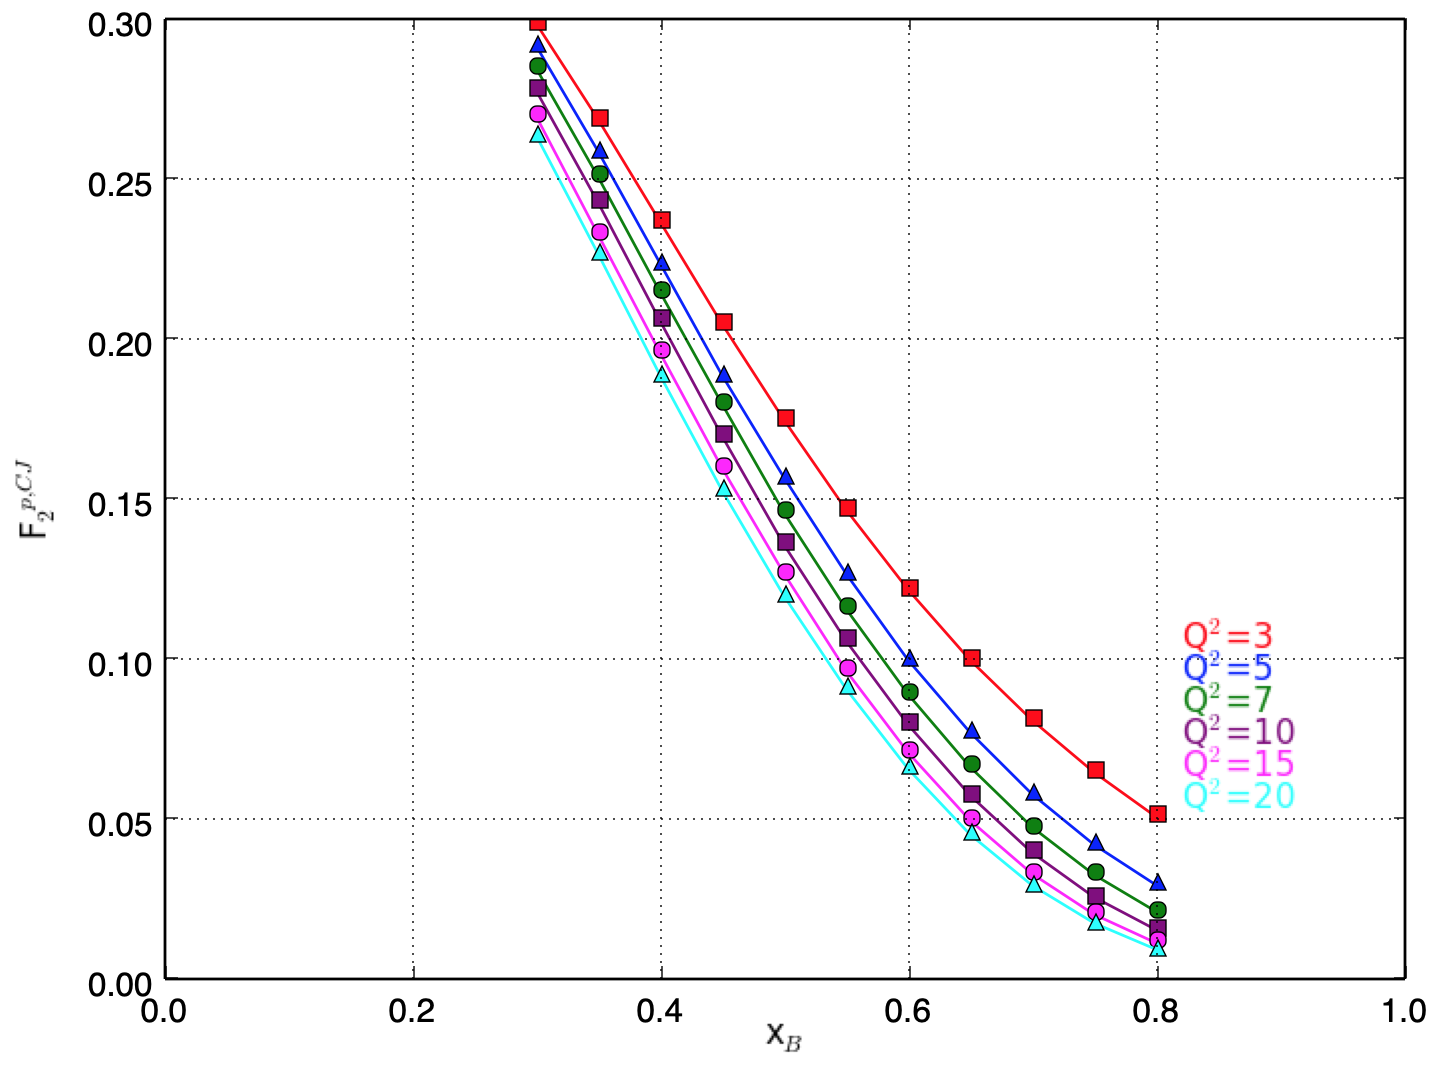
\includegraphics[width=\textwidth]{plots/p_CJ.png}
\end{minipage}\hfill\begin{minipage}{0.5\textwidth}
 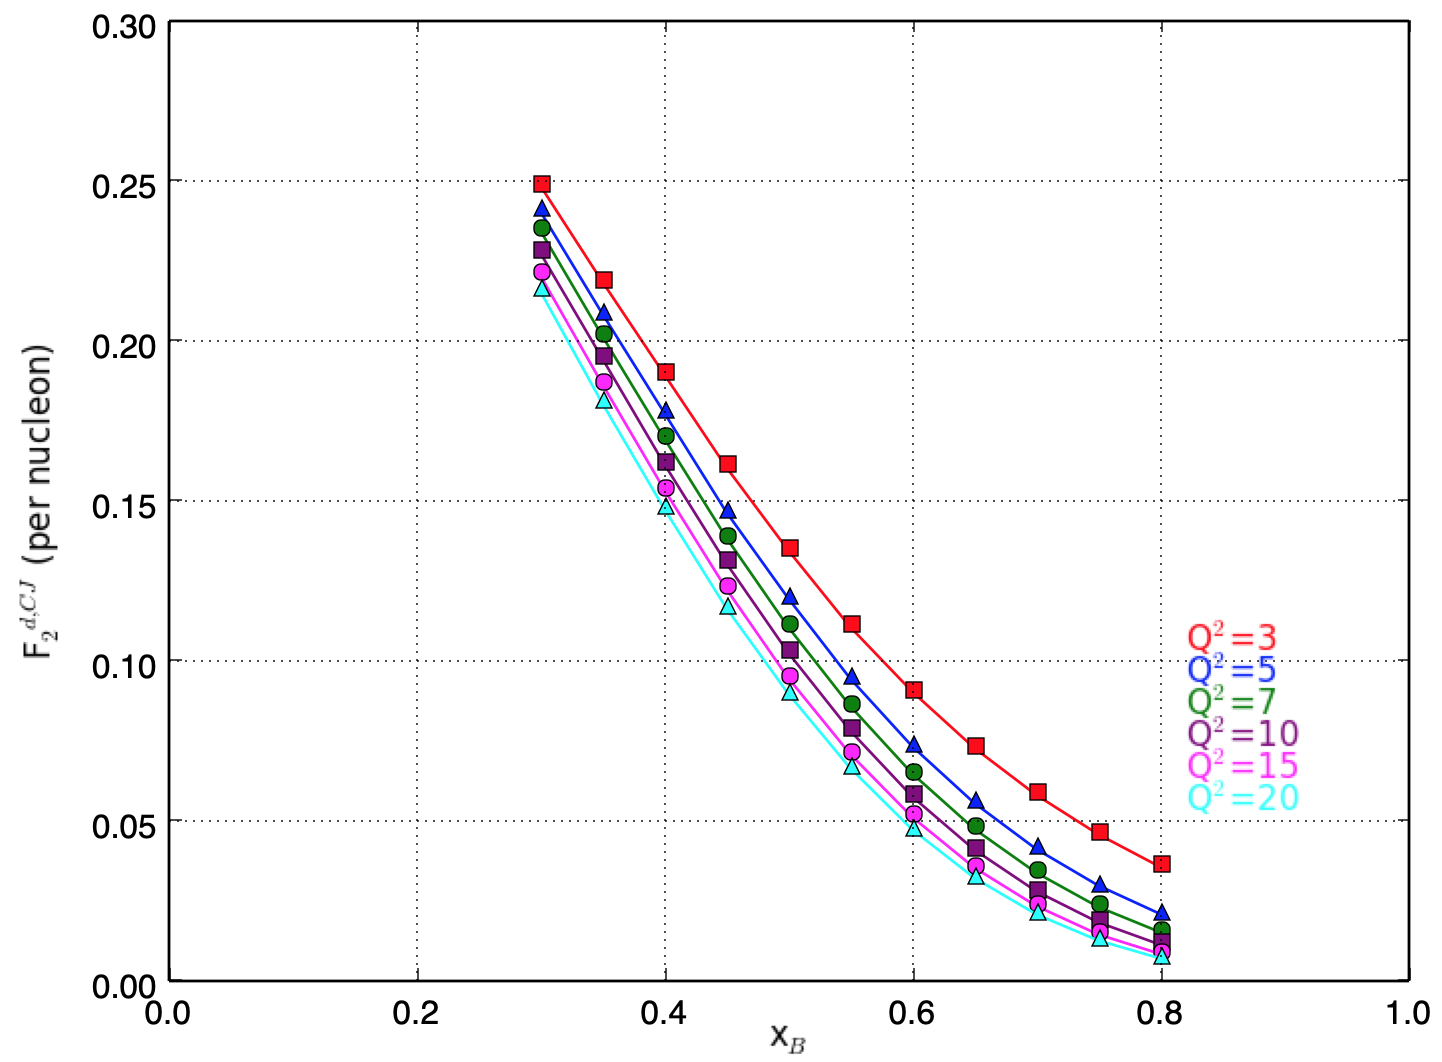
\includegraphics[width=\textwidth]{plots/d_CJ.png}
 \end{minipage}
  \caption[Proton and deuteron from CJ15]{Left: The proton structure function from the CJ15 fit is shown as a function of $x_B$ for various fixed $Q^2$. Right: The deuteron structure function from the CJ15 fit is shown as a function of $x_B$ for various fixed $Q^2$.}
  \label{fig:pd_CJ15}
\end{figure} 
 
 \begin{figure}
\begin{minipage}{0.5\textwidth}
 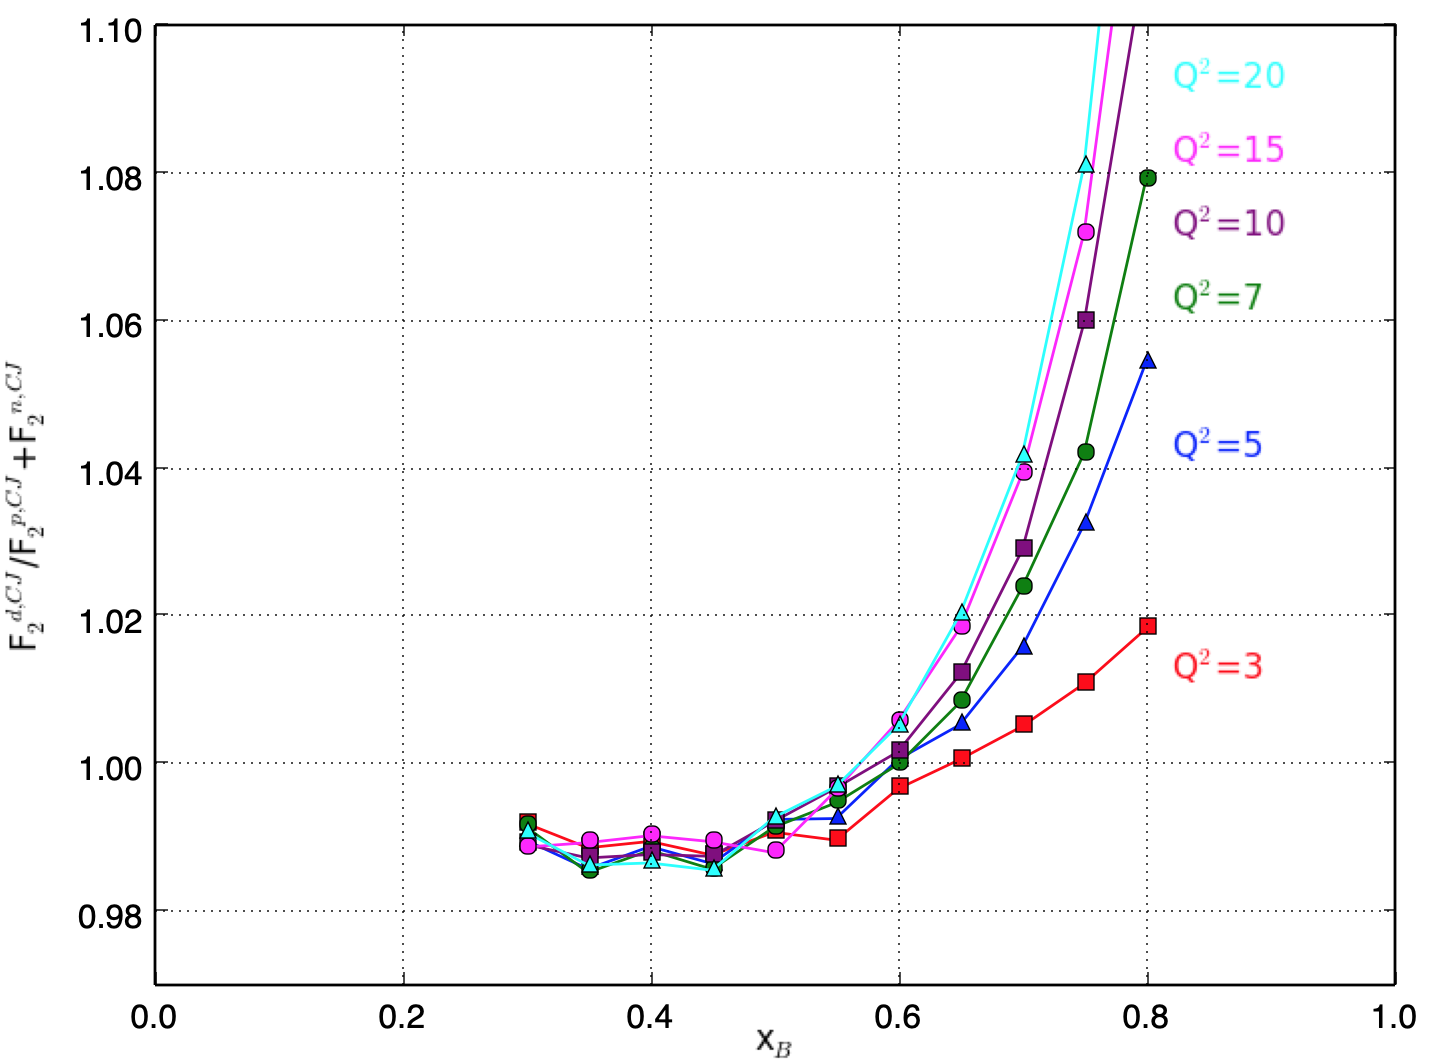
\includegraphics[width=\textwidth]{plots/dpn_allCJ.png}
\end{minipage}\hfill\begin{minipage}{0.5\textwidth}
 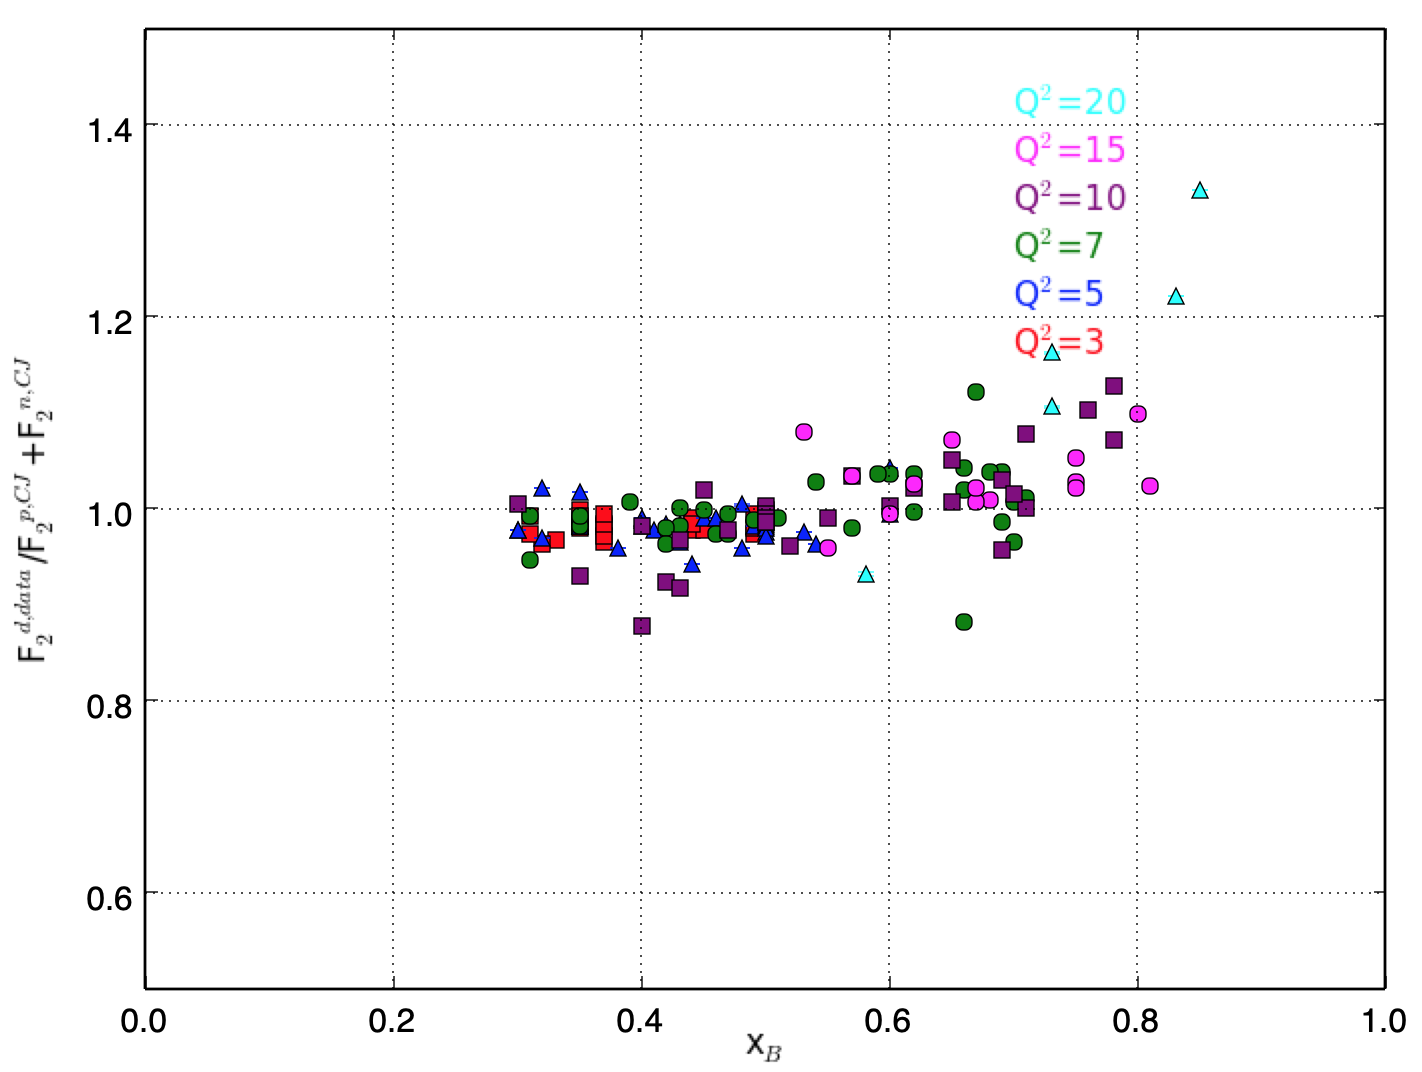
\includegraphics[width=\textwidth]{plots/deuterium_q2.png}
 \end{minipage}
  \caption[]{Left: The deuteron structure function divided by the sum of the free proton and free neutron structure functions from the CJ15 fit is shown for various $Q^2$. This ratio roughly shows the magnitude of the nuclear effects in the deuteron. The $Q^2$ dependence shows significant spread above $x_B=0.6$ where the ratio begins to increase. Right: The global Whitlow deuterium data from SLAC~\cite{XS_d} is shown divided by the sum of the free proton and free neutron structure functions from the CJ15 fit.}
  \label{fig:dpn_cj}
\end{figure}  
 
 
 
  \begin{figure}
\begin{minipage}{0.5\textwidth}
 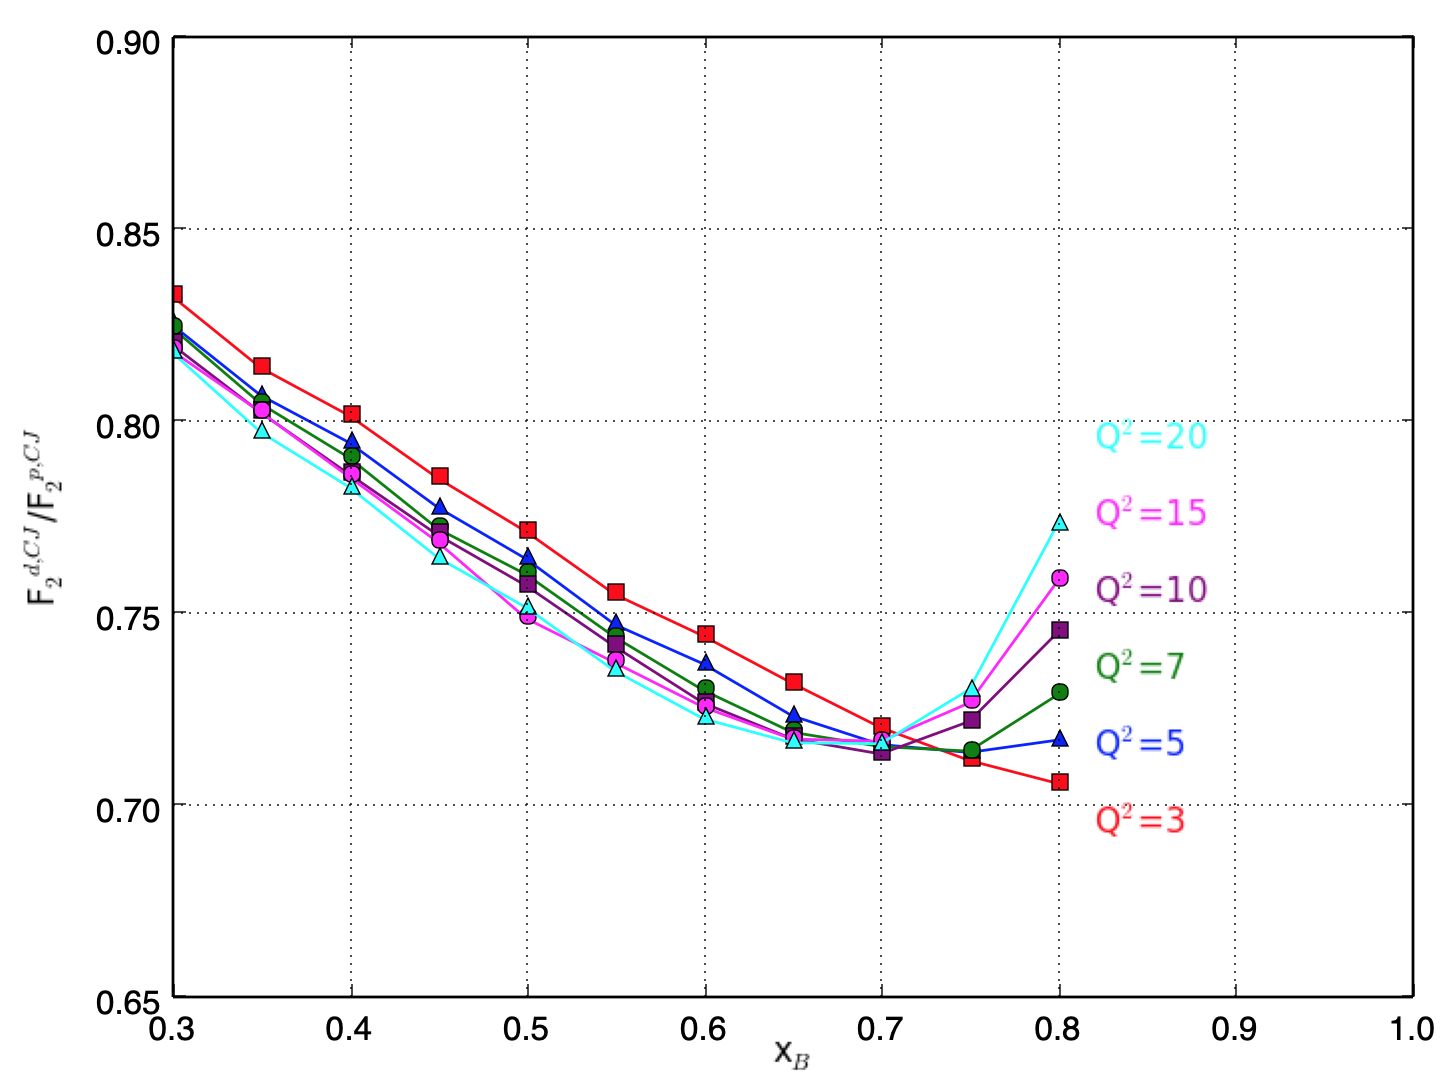
\includegraphics[width=\textwidth]{plots/dpratio_CJ.png}
\end{minipage}\hfill\begin{minipage}{0.5\textwidth}
 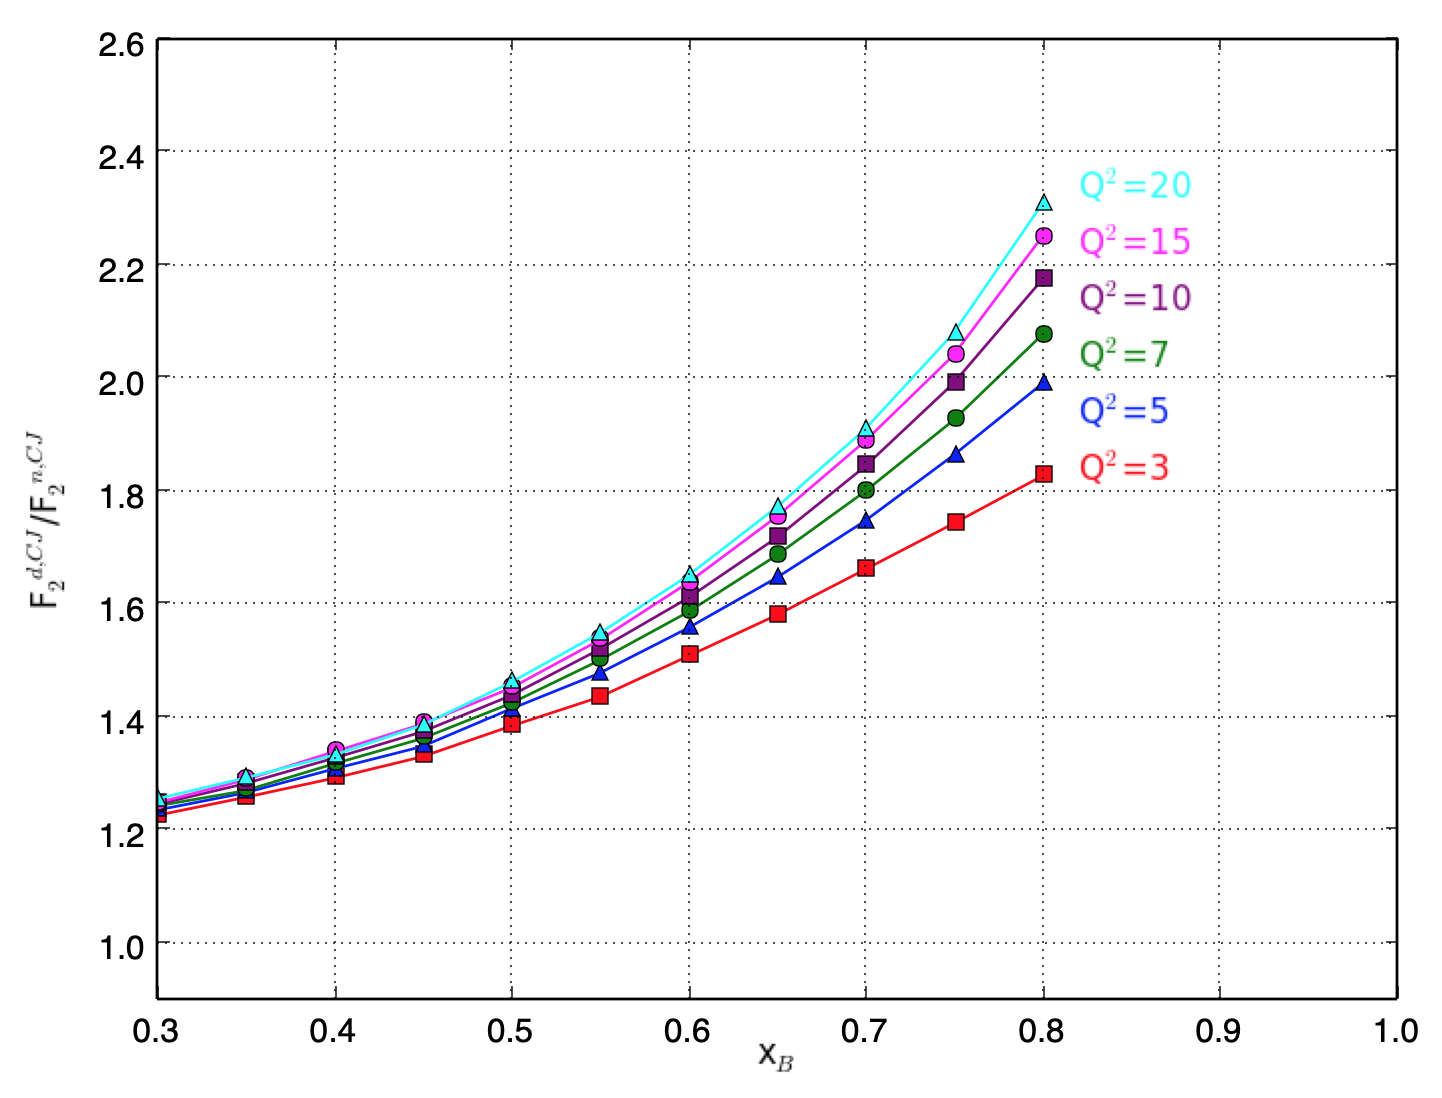
\includegraphics[width=\textwidth]{plots/dnratio_CJ.png}
 \end{minipage}
  \caption[Deuteron ratios from CJ15]{Left: The deuterium structure function from the CJ15 fit is shown as a ratio to the proton structure function from CJ15 for various $Q^2$. Right: The deuterium structure function from the CJ15 fit is shown as a ratio to the neutron structure function from CJ15 for various $Q^2$.}
  \label{fig:dratio_cj}
\end{figure} 

\section{Structure function extraction from the E139 cross sections}

Most experiments officially publish the extracted $F_2$ ratios. For this analysis, the experimental cross sections were desirable for the flexibility to construct and study the $F_2$ ratios for the nucleus of interest relative to various free nucleon quantities. The SLAC E139 experiment published the experimental cross sections for the following nuclei: deuterium, helium, beryllium, carbon, aluminum, calcium, iron, silver and gold. The cross sections include published statistical and systematic errors. The $F_2$ structure function for each nucleus is extracted from the cross section using the relationship shown in Equation~\eqref{eq:f2eqn}.

\begin{equation}
F_2 = \dfrac{d^2\sigma}{d\Omega dE'}\dfrac{1+R}{1+\epsilon R}\dfrac{K\nu}{4\pi^2\alpha\Gamma (1+\nu^2/Q^2)}
\label{eq:f2eqn}
\end{equation}

From Equation~\eqref{eq:f2eqn}, $\epsilon$, $K$, and $\Gamma$ are defined by the usual quantities of the electron scattering kinematics in Equation~\eqref{eq:f2eqndetails}. These quantities include the measured scattering angle $\theta$, the momentum transfer $Q^2$, the energy transfer $\nu$, the scattered electron energy $E'$, the mass of the proton $M$, and the squared invariant mass $W^2$.

\begin{align}
\epsilon=&(1+2\dfrac{\nu^2+Q^2}{Q^2}tan^2\dfrac{\theta}{2})^{-1}\\
K=&\dfrac{W^2-M^2}{2M}\\
\Gamma=&\dfrac{\alpha KE'}{2\pi^2Q^2E(1-\epsilon)}
\label{eq:f2eqndetails}
\end{align}

For most published cross section ratios, corrections are applied to account for the excess of neutrons in asymmetric nuclei. This correction is referred to as the ``isoscalar correction" and is defined in Equation~\eqref{eq:isocorr}. While this correction is not applied in this paper for the $F_2$ ratios per free proton and free neutron, it is relevant for accurately reconstructing the published $F_2^A$/$F_2^d$ cross sections as in most analyses. 

\begin{equation}
f_{iso}^A = \dfrac{\dfrac{1}{2}(1+F_2^n/F_2^p)}{\dfrac{1}{A}(Z+(A-Z)F_2^n/F_2^p)}
\label{eq:isocorr}
\end{equation}

From the analysis described in this section, the carbon and gold $F_2^A/F_2^d$ ratios are reconstructed (with the iso-scalar correction applied to gold) and compared to the published ratios in the EMC and NMC experiments as shown in Fig.~\ref{fig:emc_ratios}.

\begin{figure}[H]
  \centering
      	  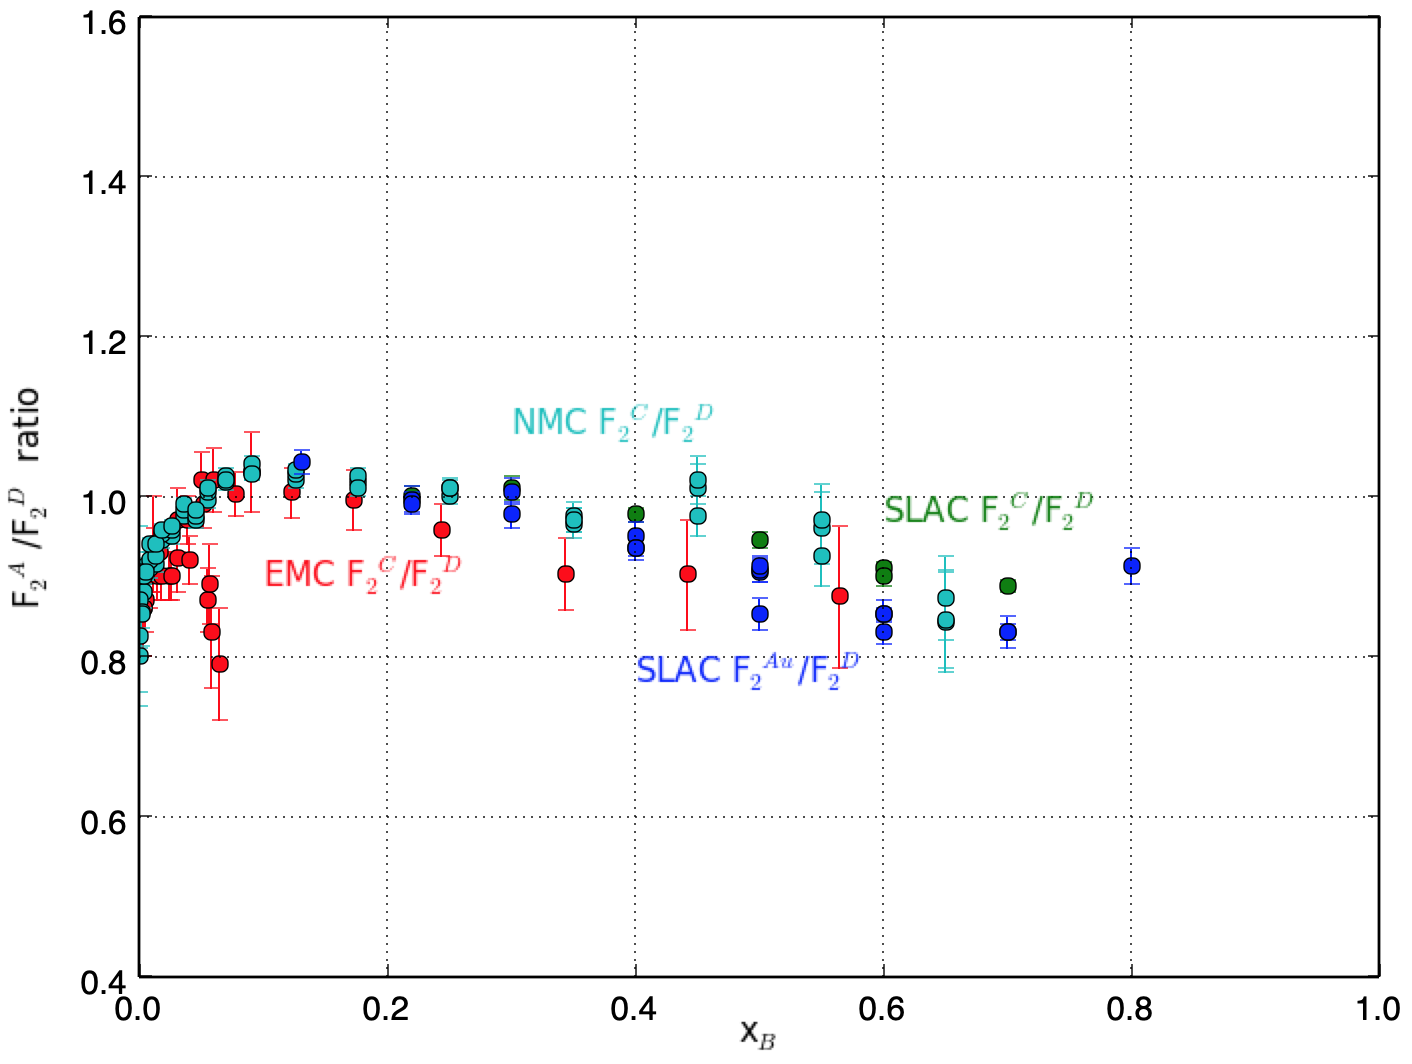
\includegraphics[width=0.5\textwidth]{plots/emc_ratios_data.png}
 	 \caption[EMC ratios for various data]{The published structure function ratios per nucleon for carbon and gold are shown from SLAC, NMC, and the EMC experiments.}
  \label{fig:emc_ratios}
 \end{figure}
 
 The carbon ratio from the SLAC E139 experiment is consistent with the ratio found in the EMC and NMC experiments, and the carbon exhibits a shallower slope with respect to $x_B$ as compared to the heavier, iso-scalar corrected gold ratio. 

\section{General observations}
 
  \begin{figure}
\begin{minipage}{0.5\textwidth}
 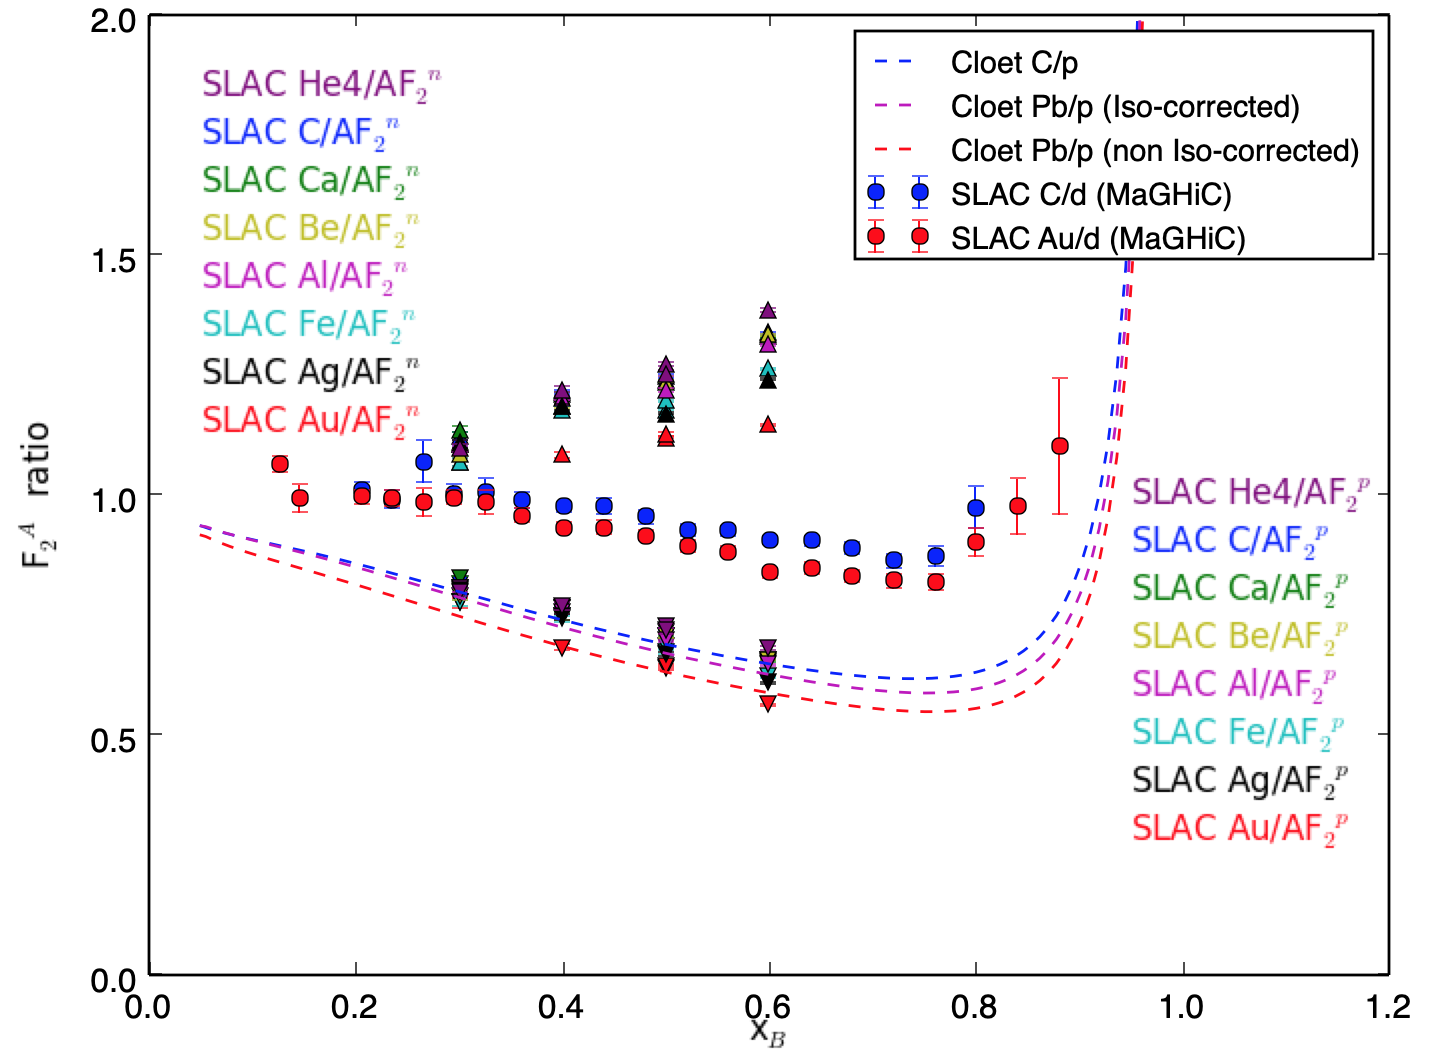
\includegraphics[width=\textwidth]{plots/Anp_data_ratio.png}
\end{minipage}\hfill\begin{minipage}{0.5\textwidth}
 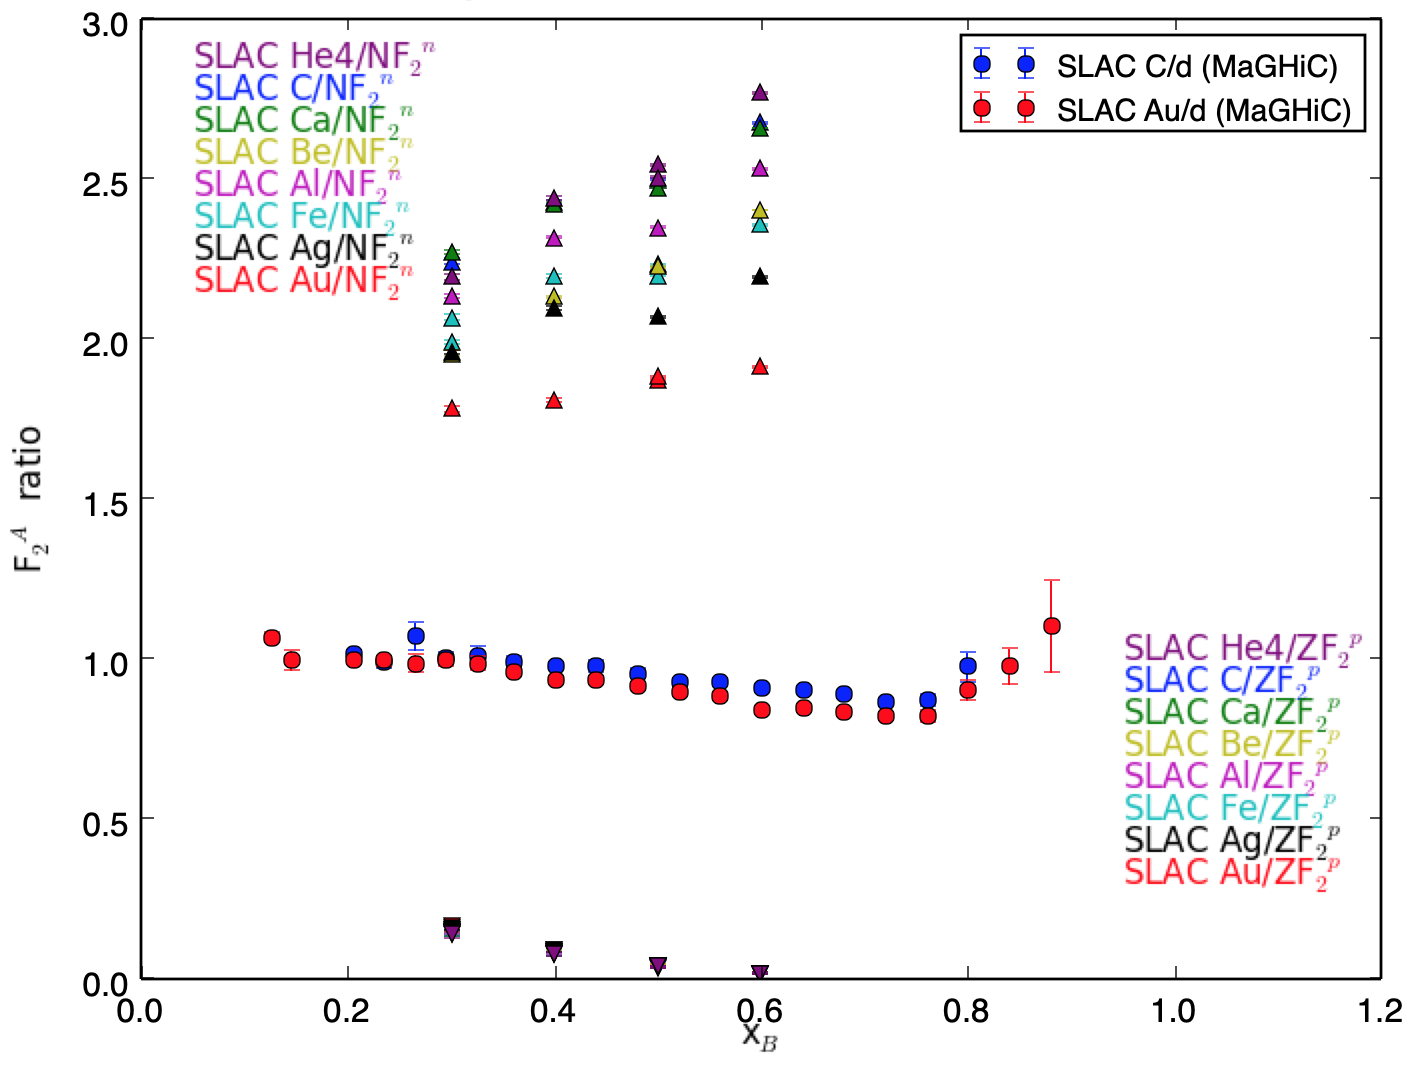
\includegraphics[width=\textwidth]{plots/AZNnp_data_ratio.png}
 \end{minipage}
  \caption[$F_2^A$ ratio to $F_2^n$ and $F_2^p$]{Left: $F_2^A$ calculated from the published SLAC E139 cross sections is taken as a ratio per nucleon to $F_2^n$ and $F_2^p$, separately. The published EMC ratios for carbon and gold~\cite{Malace:2014uea} are shown for reference as $F_2^A/F_2^d$ per nucleon. Theory predictions for the $F_2^A$ structure function per nucleon as a ratio to $F_2^p$ are shown. Right: $F_2^A$ calculated from the published SLAC E139 cross sections is taken as a ratio per neutron or proton and $F_2^n$ and $F_2^p$, separately. The published EMC ratios for carbon and gold~\cite{Malace:2014uea} are shown for reference.}
  \label{fig:data_np_ratio}
\end{figure}  
 
 
\section{Deuterium nuclear effects and heavier nuclei}

\subsection{Deuterium}



plots: include d/n or n/d of Whitlow+BONUS to show Q2 dependency

\subsection{Heavier nuclei}


  \begin{figure}
\begin{minipage}{0.5\textwidth}
 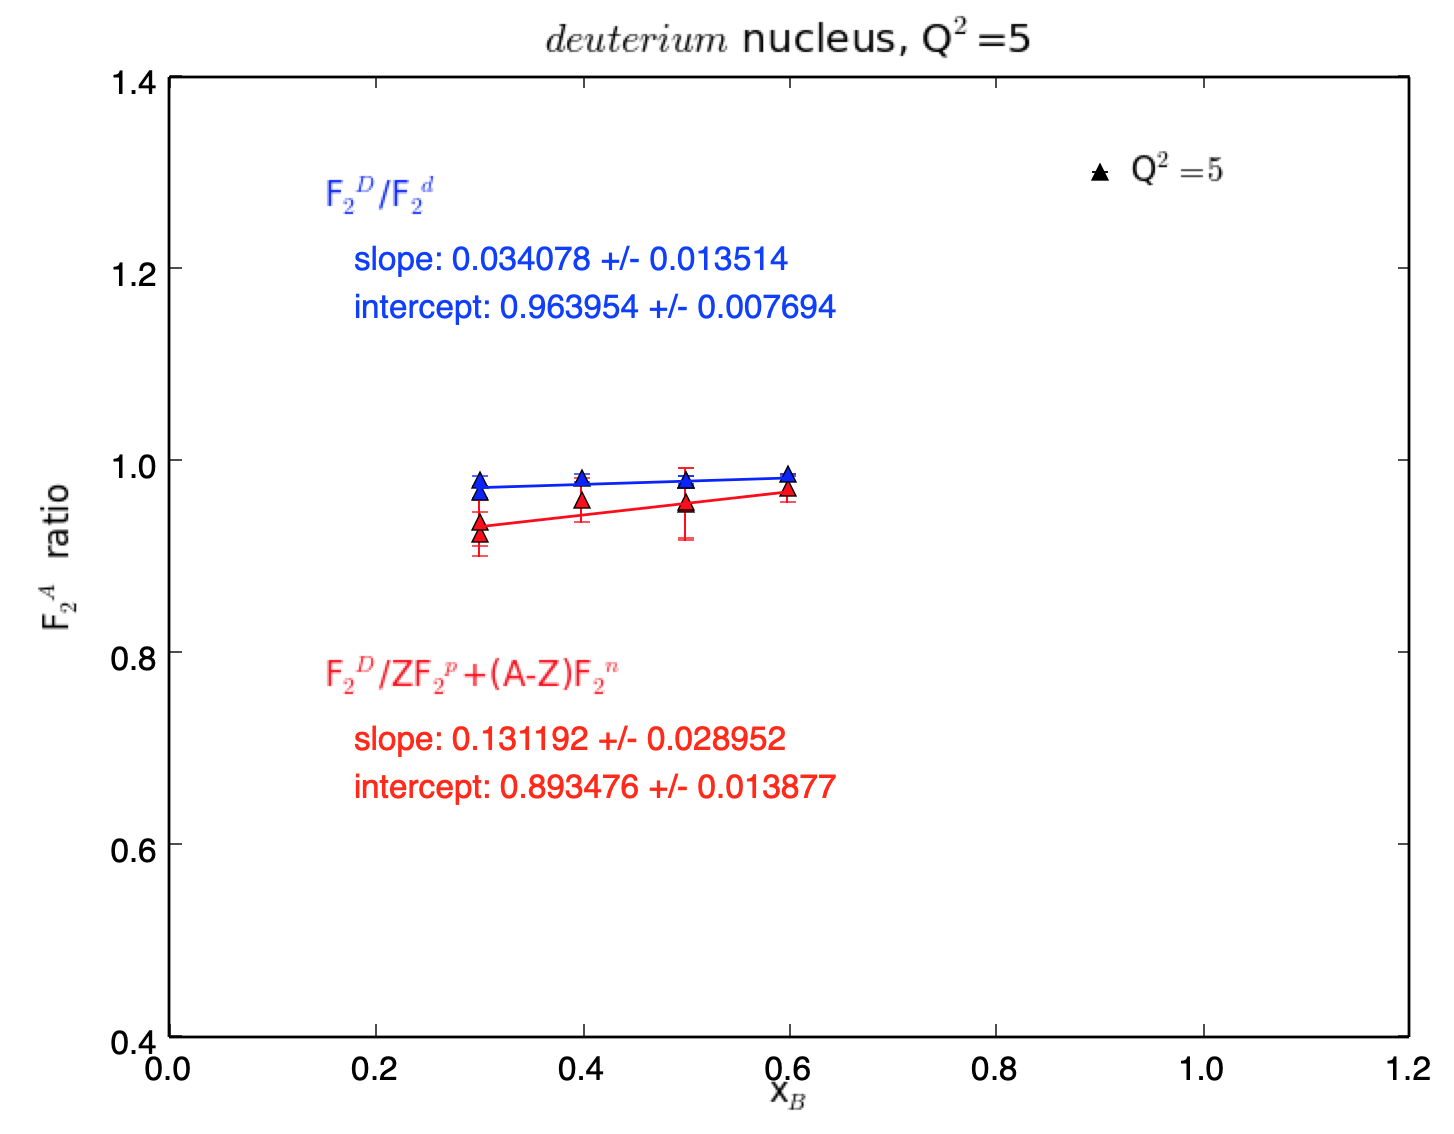
\includegraphics[width=\textwidth]{plots/q2_5/q2_5_D.png}
\end{minipage}\hfill\begin{minipage}{0.5\textwidth}
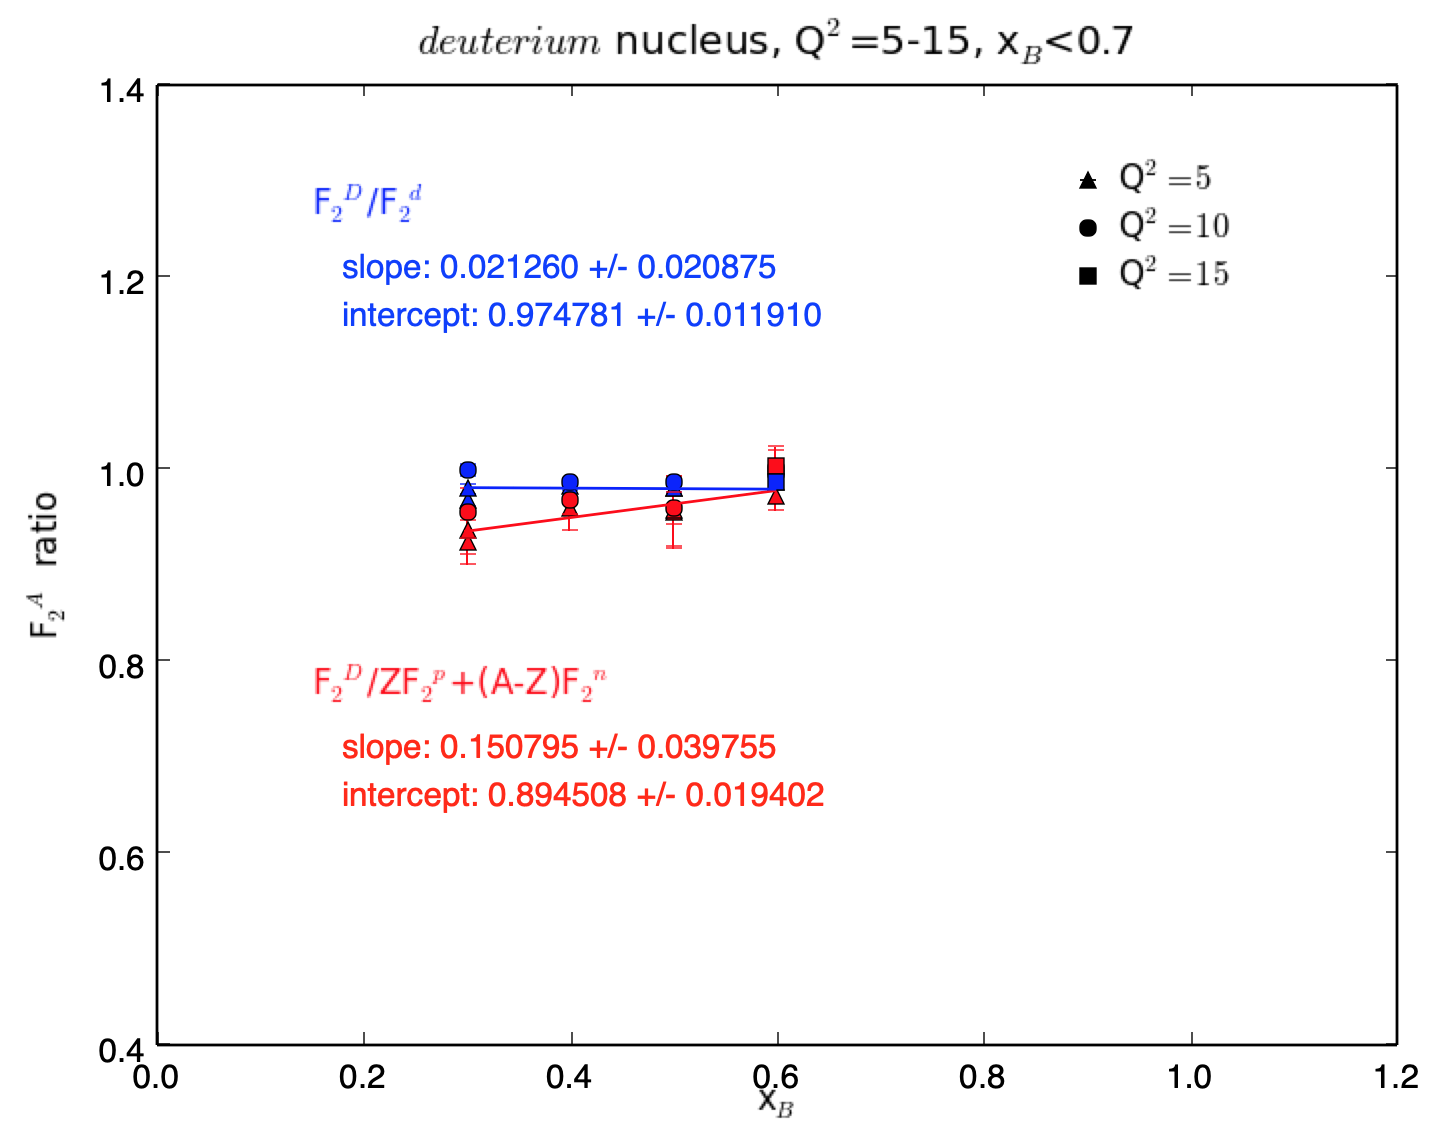
\includegraphics[width=\textwidth]{plots/q2_all_x_l7/q2_all_x_l7_D.png}
\end{minipage}\hfill\begin{minipage}{0.5\textwidth}
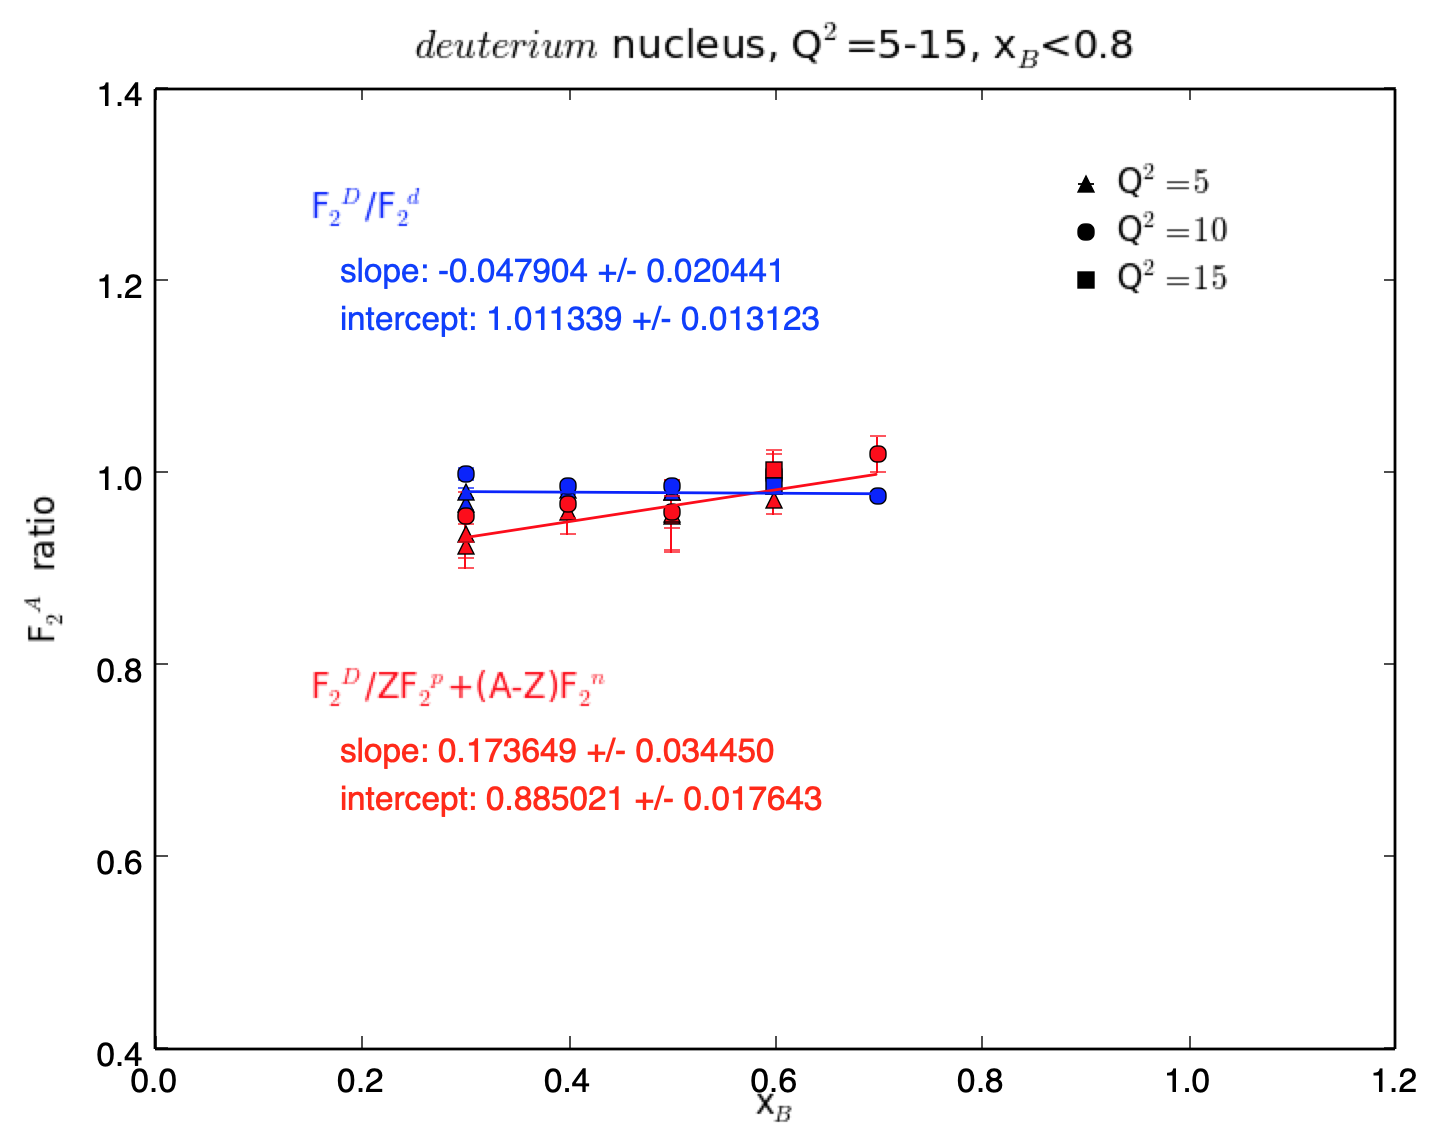
\includegraphics[width=\textwidth]{plots/q2_all_x_all/all_D.png}
\end{minipage}
  \caption[]{Linear fits to the deuterium target data with cuts on $Q^2$ and $x_B$.}
  \label{fig:fits_D}
\end{figure}  

 \begin{figure}
\begin{minipage}{0.5\textwidth}
 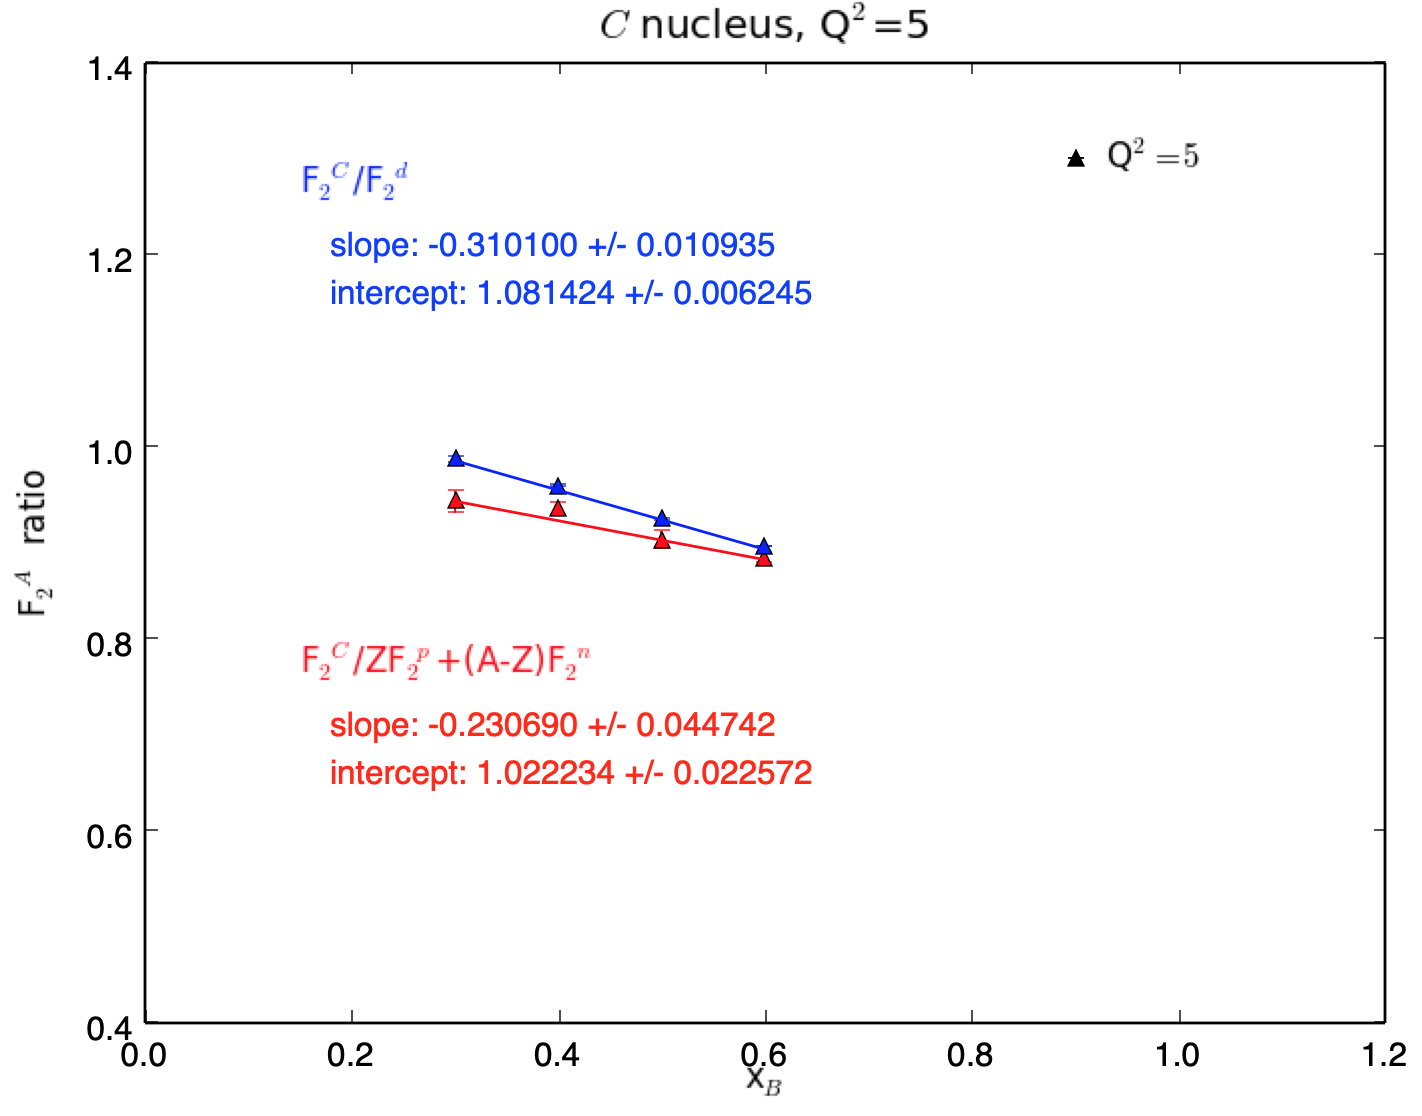
\includegraphics[width=\textwidth]{plots/q2_5/q2_5_C.png}
\end{minipage}\hfill\begin{minipage}{0.5\textwidth}
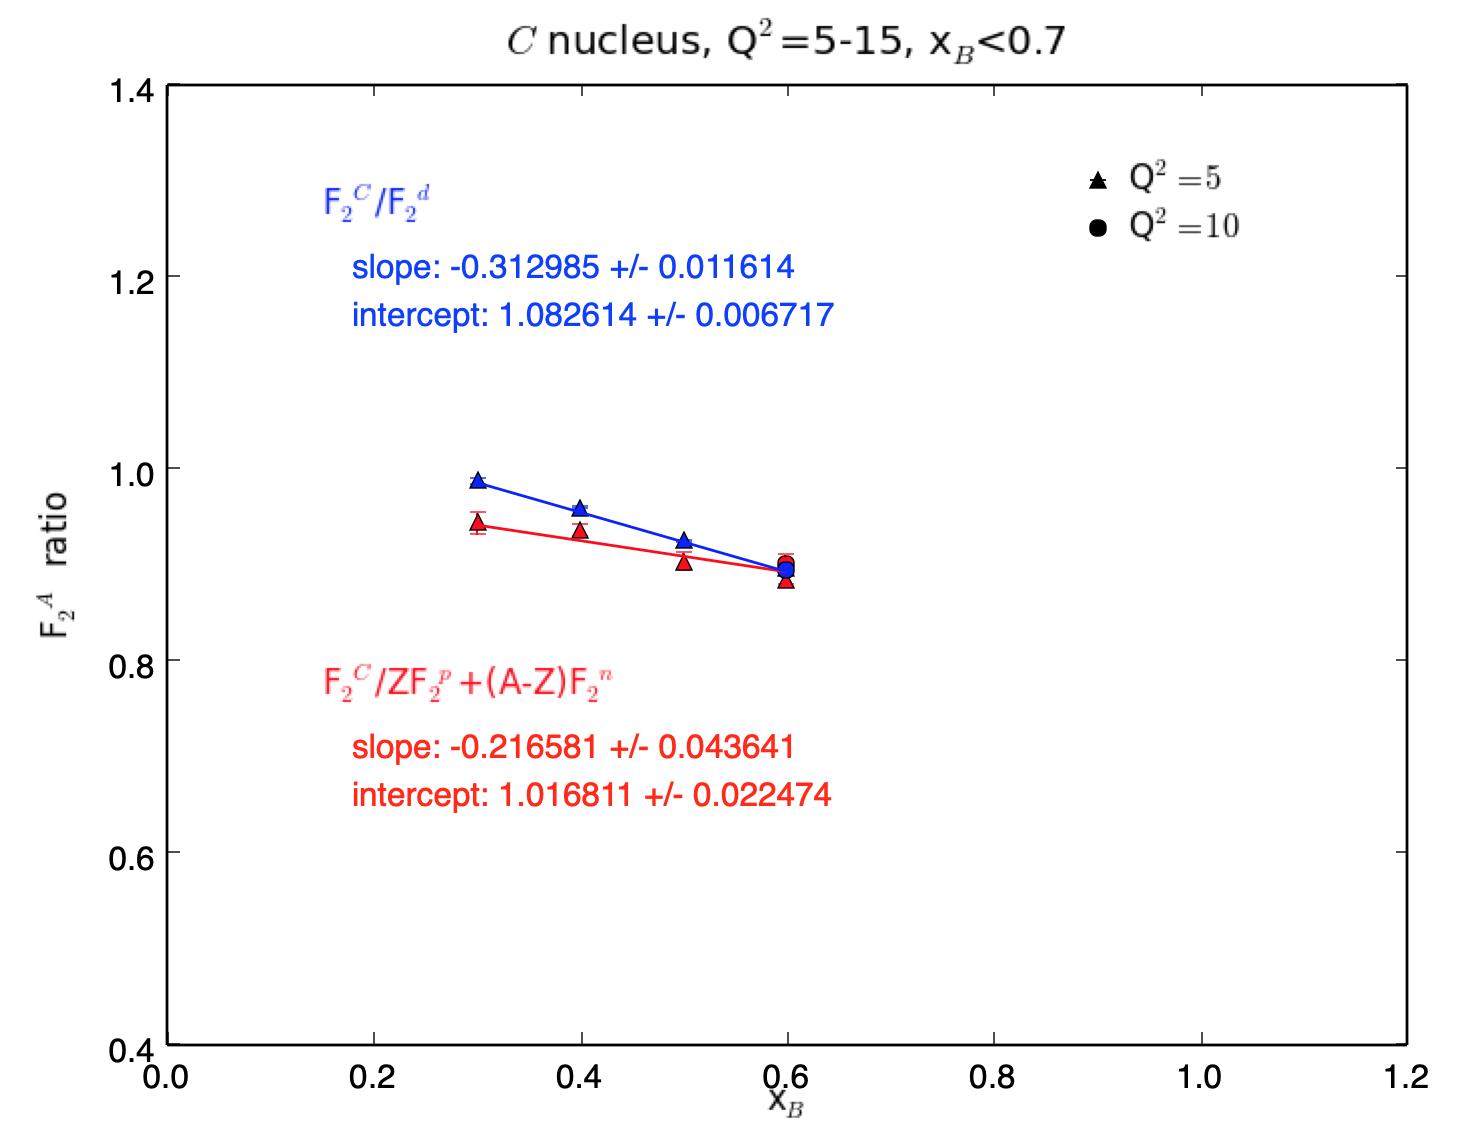
\includegraphics[width=\textwidth]{plots/q2_all_x_l7/q2_all_x_l7_C.png}
\end{minipage}\hfill\begin{minipage}{0.5\textwidth}
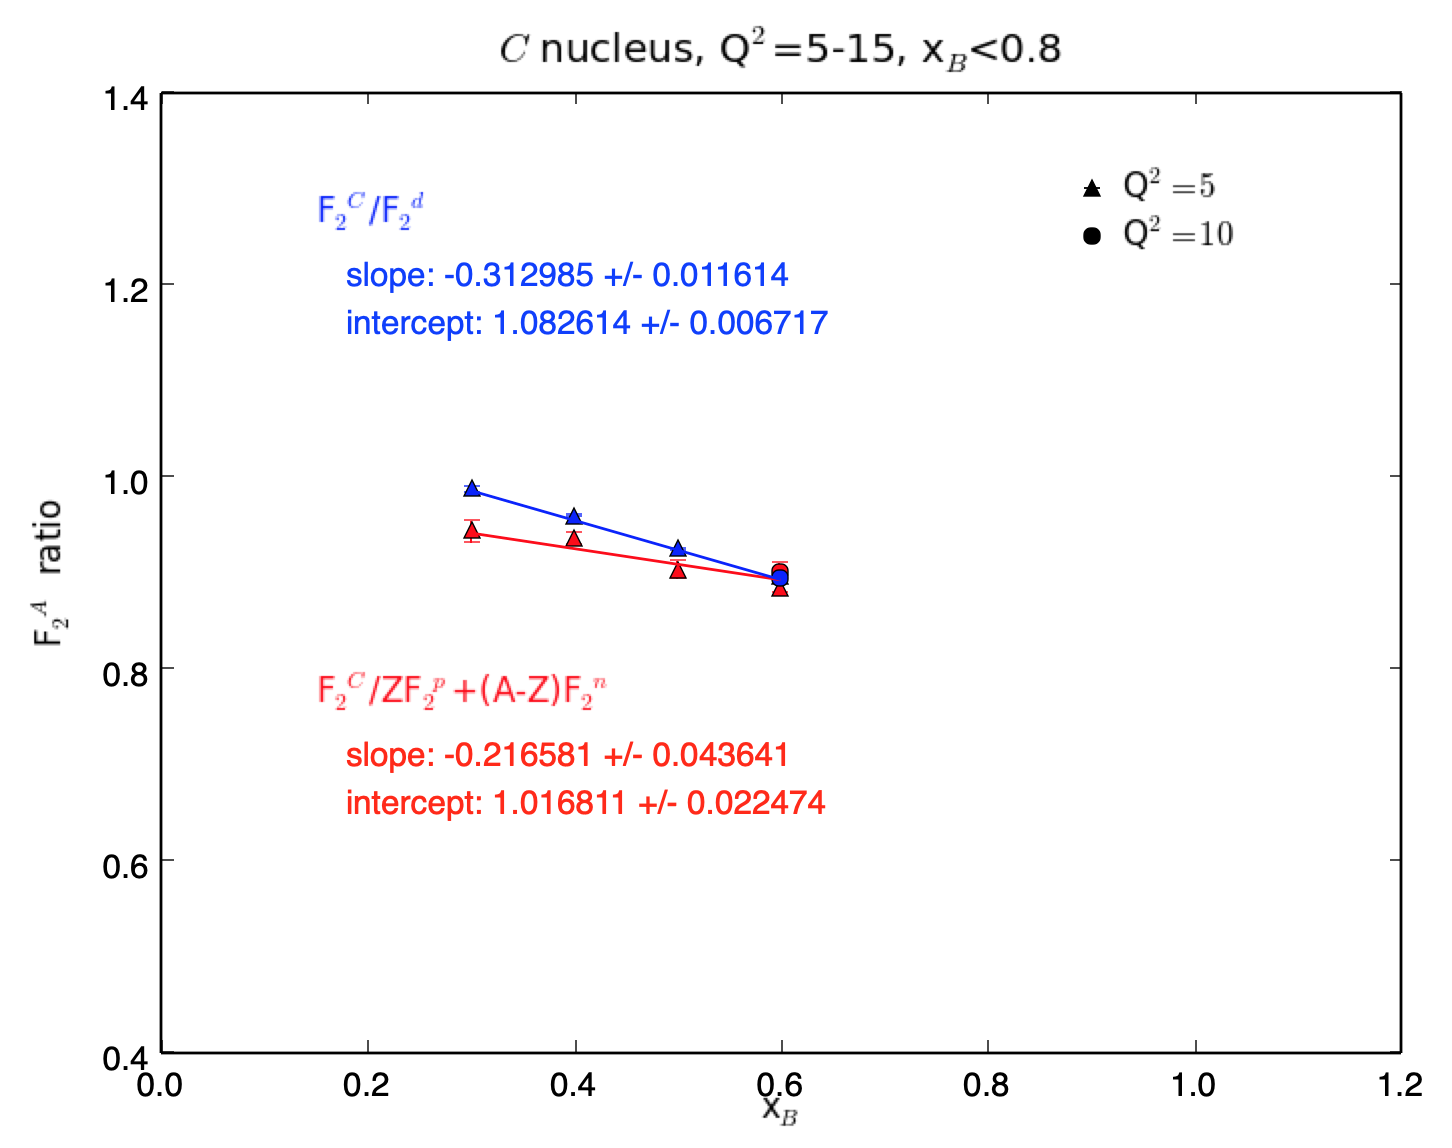
\includegraphics[width=\textwidth]{plots/q2_all_x_all/all_C.png}
\end{minipage}
  \caption[]{Linear fits to the $C$ target data with cuts on $Q^2$ and $x_B$.}
  \label{fig:fits_C}
\end{figure}   

 \begin{figure}
\begin{minipage}{0.5\textwidth}
 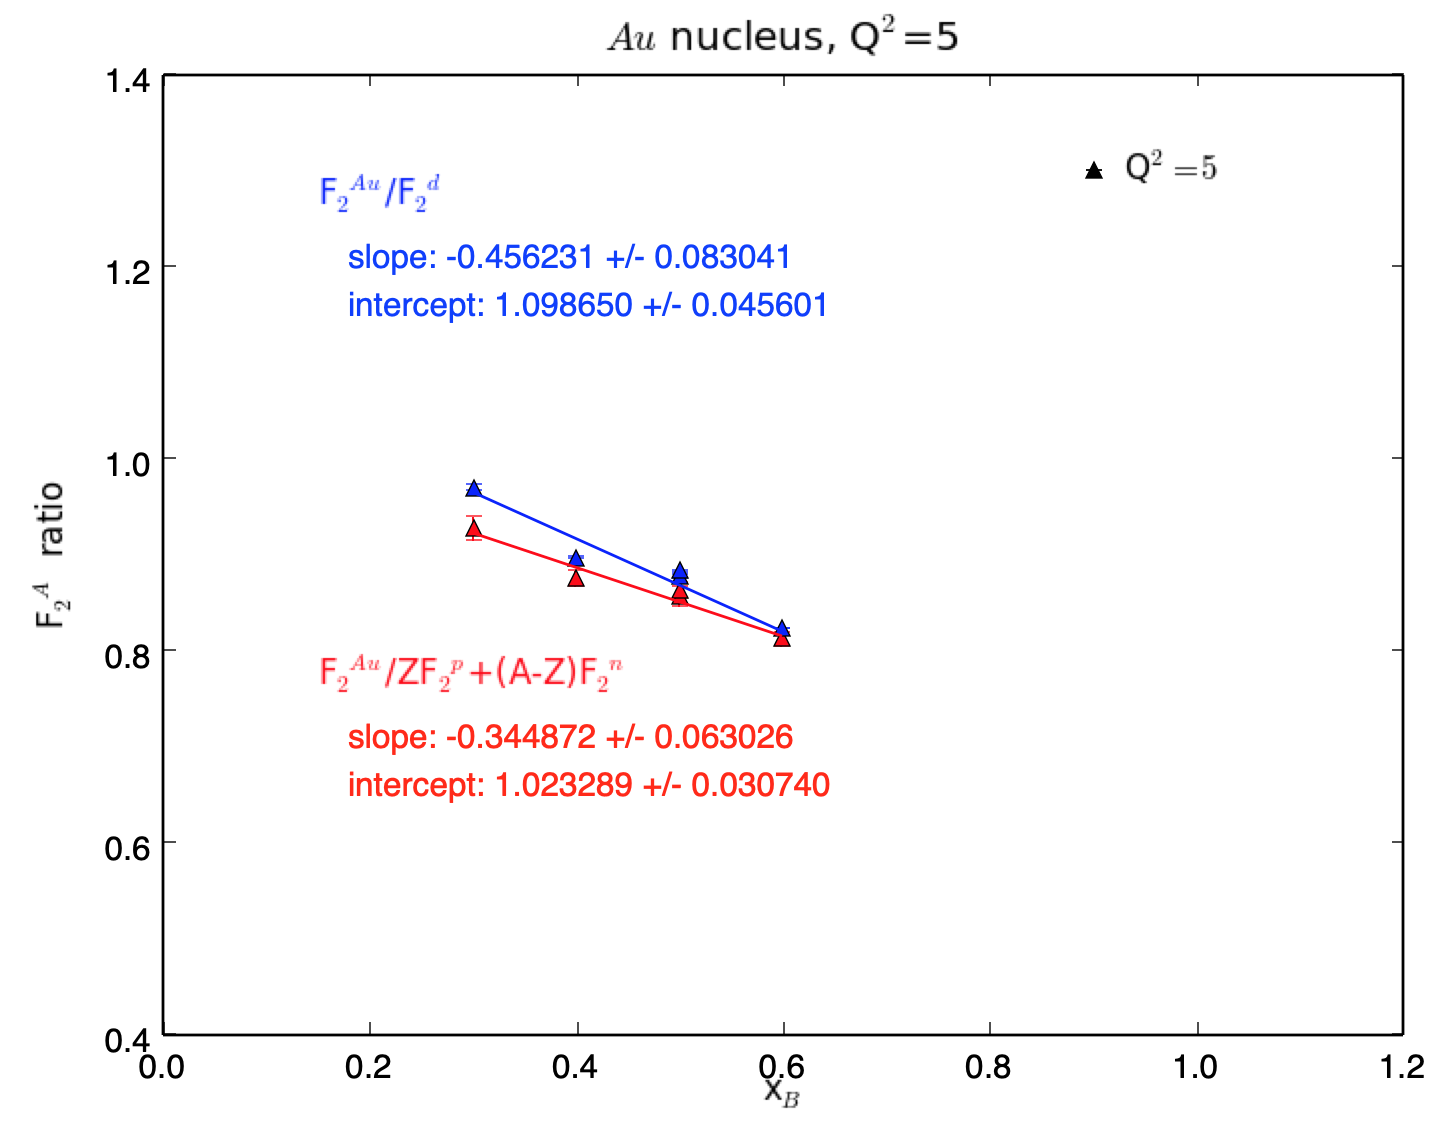
\includegraphics[width=\textwidth]{plots/q2_5/q2_5_Au.png}
\end{minipage}\hfill\begin{minipage}{0.5\textwidth}
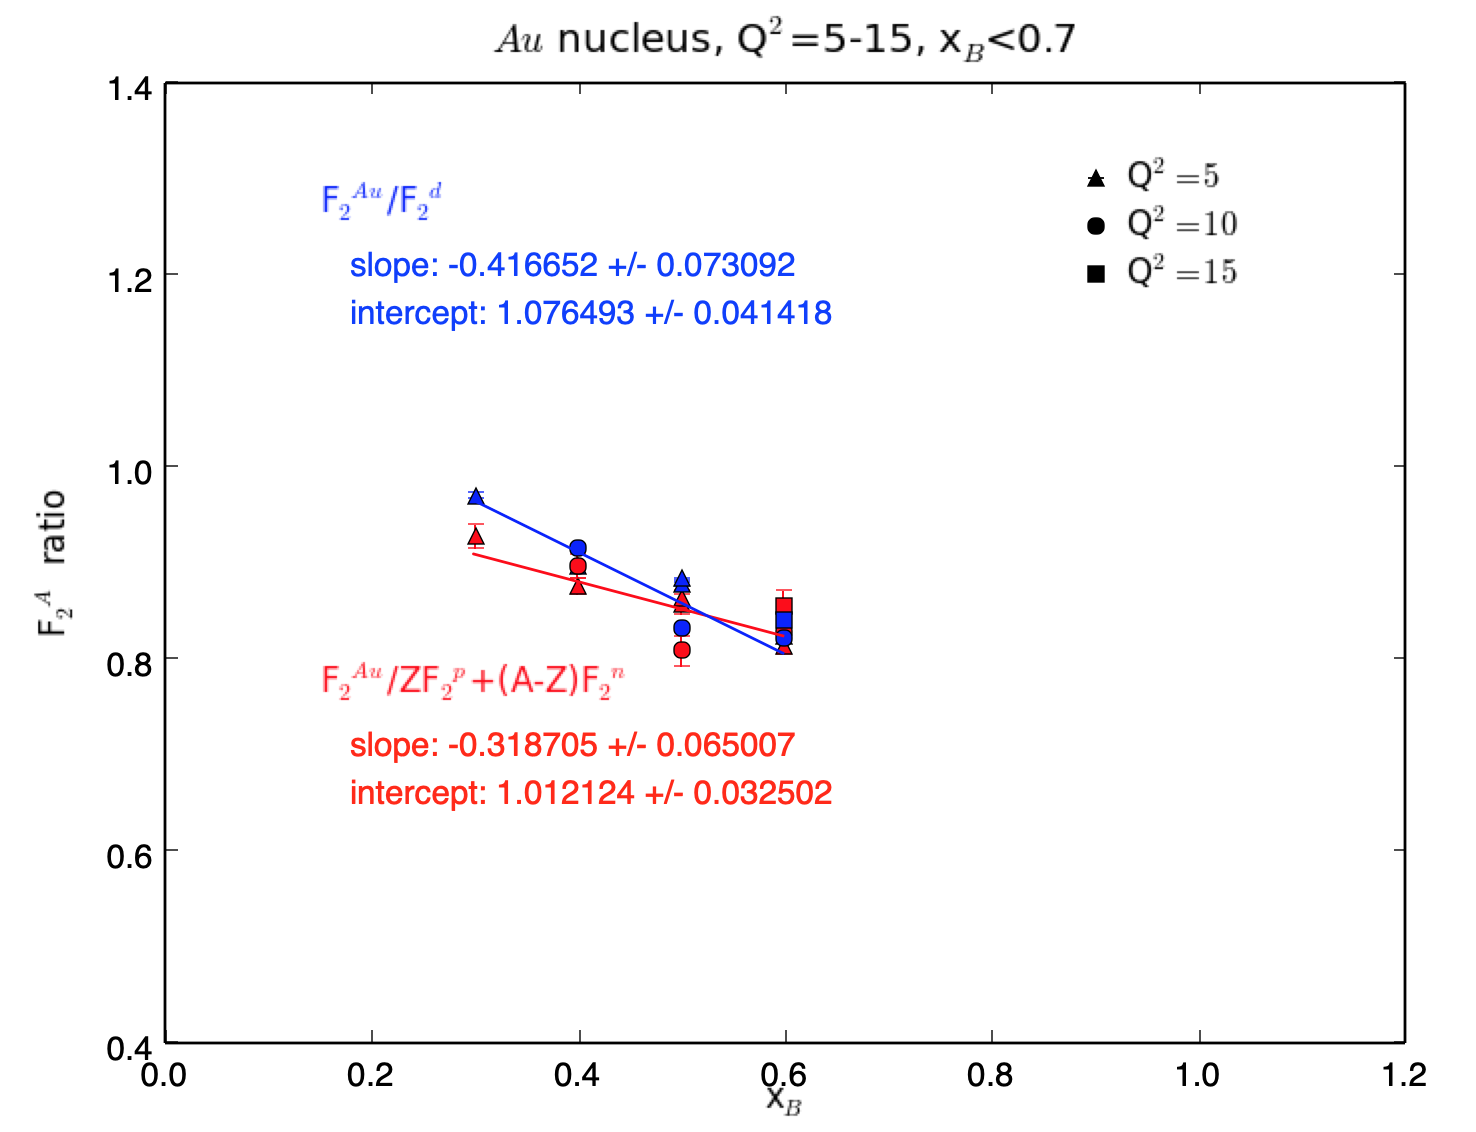
\includegraphics[width=\textwidth]{plots/q2_all_x_l7/q2_all_x_l7_Au.png}
\end{minipage}\hfill\begin{minipage}{0.5\textwidth}
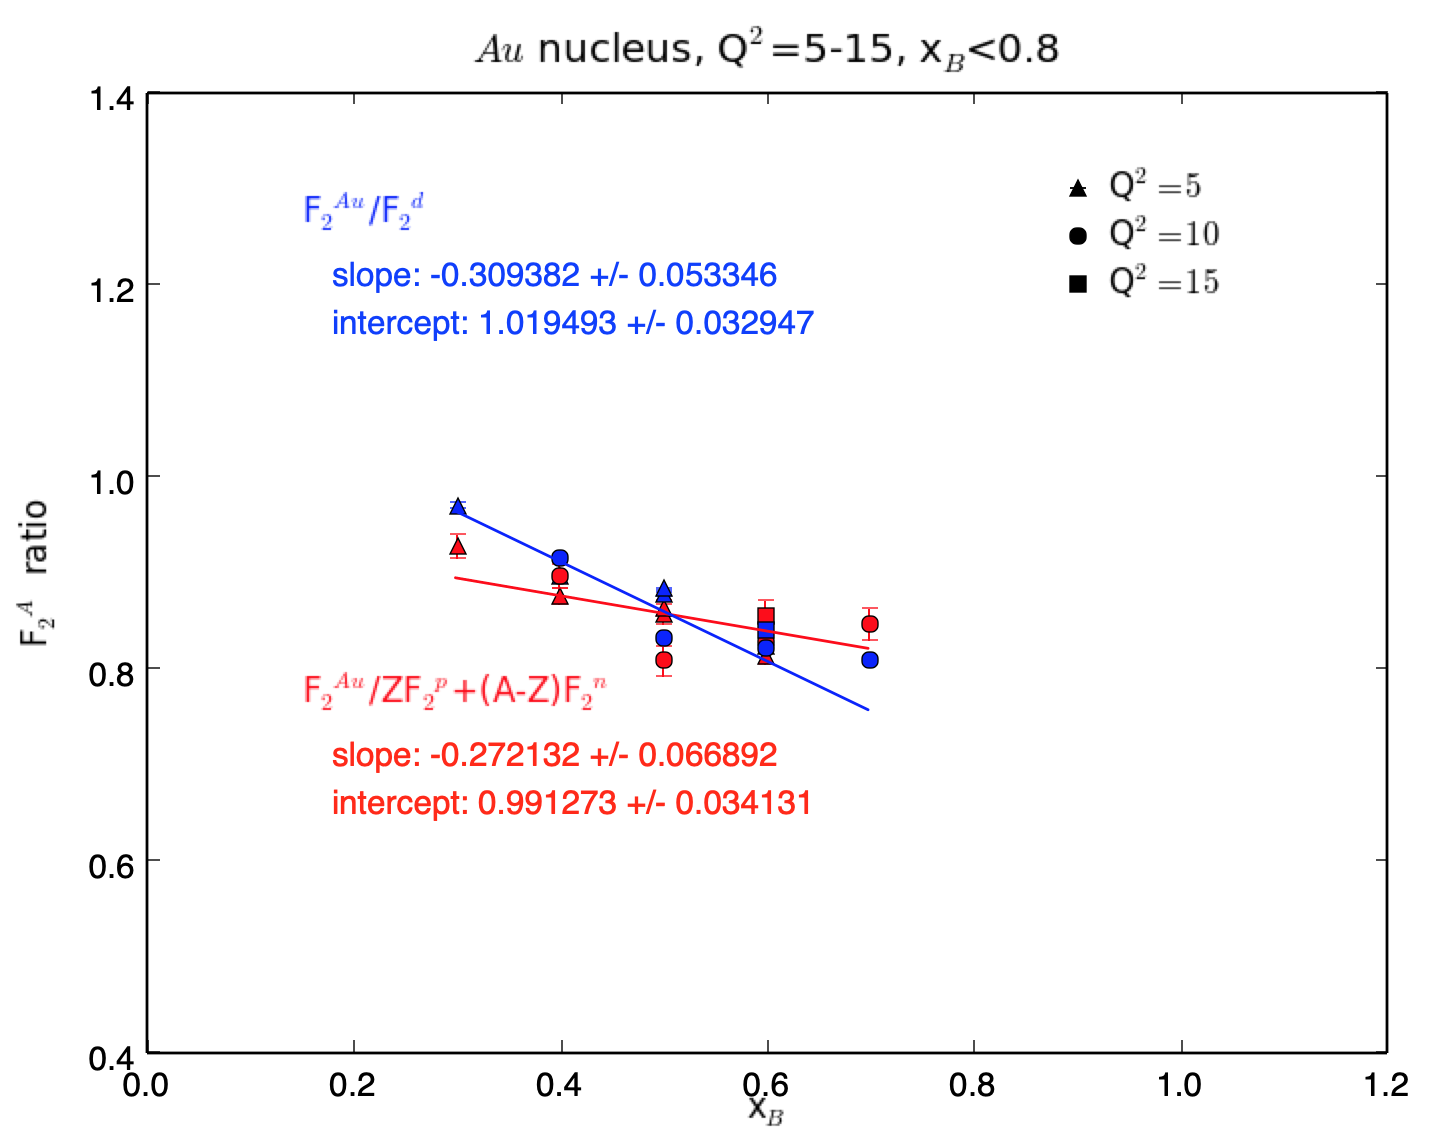
\includegraphics[width=\textwidth]{plots/q2_all_x_all/all_Au.png}
\end{minipage}
  \caption[]{Linear fits to the $Au$ target data with cuts on $Q^2$ and $x_B$.}
  \label{fig:fits_Au}
\end{figure}   

\begin{table}[htb!]
\caption{\label{SlopeFits} Summary of linear fits to $x_B$ where $Q^2=5$.}
\centering
\begin{tabular}{ | C{2.5cm} | C{2cm} | C{2cm} | C{2cm} | C{2cm} | }
 \hline
 \textbf{Nucleus} & \textbf{A/d slope} & \textbf{A/d intercept} & \textbf{A/(n+p) slope} & \textbf{A/(n+p) intercept} \\ 
  \hline
deuterium & 0.034078+/-0.013514	& 0.963954+/-0.007694 & 0.131192+/-0.028952 &	0.893476+/-0.013877 \\ 
  \hline
  He4 & -0.139559+/-0.041514	 & 1.010444+/-0.023729 & -0.054561+/-0.053741 & 0.947196+/-0.027083 \\ 
 \hline
 Be & -0.153575+/-0.004225	 &1.020754+/-0.002375 &-0.064459+/-0.041653&	0.955925+/-0.020121\\ 
  \hline
   C & -0.310100+/-0.010935	& 1.081424+/-0.006245 & -0.230690+/-0.044742	&1.022234+/-0.022572  \\ 
  \hline
    Al &-0.308688+/-0.058075 &	1.074479+/-0.032618 & -0.241920+/-0.085474 &	1.021834+/-0.042052 \\ 
  \hline
 Ca &-0.327402+/-0.048885 &	1.085172+/-0.027035 & -0.27227+/-0.051774 &	1.037505+/-0.025103 \\ 
  \hline  
  Fe & -0.368335+/-0.041561&	1.085849+/-0.022646& -0.286425+/-0.062250 &	1.024809+/-0.029771 \\ 
  \hline 
  Ag & -0.423013+/-0.087616 &	1.119710+/-0.048607 & -0.360732+/-0.113255	& 1.068858+/-0.055132 \\ 
  \hline 
   Au & -0.456231+/-0.083041	&1.098650+/-0.045601 & -0.344872+/-0.063026 &	1.023289+/-0.030740\\ 
  \hline 
    \end{tabular}
\end{table} 


\begin{table}[htb!]
\caption{\label{SlopeFits1} Summary of linear fits to $x_B$ where $Q^2=5-15$ and $x_B<0.7$.}
\centering
\begin{tabular}{ | C{2.5cm} | C{2cm} | C{2cm} | C{2cm} | C{2cm} | }
 \hline
 \textbf{Nucleus} & \textbf{A/d slope} & \textbf{A/d intercept} & \textbf{A/(n+p) slope} & \textbf{A/(n+p) intercept} \\ 
  \hline
deuterium & 0.021260+/-0.020875 &	0.974781+/-0.011910 & 0.150795+/-0.039755	& 0.894508+/-0.019402 \\ 
  \hline
  He4 &-0.118090+/-0.035769 &	0.997067+/-0.020596 & -0.016222+/-0.045129 &	0.931353+/-0.023103 \\ 
 \hline
 Be &-0.197454+/-0.083778 &	1.035493+/-0.048067 &-0.059106+/-0.030303 &	0.953386+/-0.015144\\ 
  \hline
   C &-0.312985+/-0.011614	&1.082614+/-0.006717 & -0.216581+/-0.043641	&1.016811+/-0.022474 \\ 
  \hline
    Al &-0.298244+/-0.057500	&1.070859+/-0.032829 & -0.210889+/-0.056564	&1.010775+/-0.028368 \\ 
  \hline
 Ca &-0.334267+/-0.034303&	1.088128+/-0.019560 & -0.247045+/-0.051788 &	1.027656+/-0.025990 \\ 
  \hline  
  Fe & -0.379082+/-0.040058	&1.085956+/-0.022621& -0.257315+/-0.043599 &	1.010276+/-0.021402 \\ 
  \hline 
  Ag &-0.432939+/-0.060259&	1.124006+/-0.034442 & -0.338549+/-0.081071	&1.060178+/-0.040839 \\ 
  \hline 
   Au & -0.416652+/-0.073092&	1.076493+/-0.041418 & -0.318705+/-0.065007&	1.012124+/-0.032502\\ 
  \hline 
    \end{tabular}
\end{table} 

\begin{table}[htb!]
\caption{\label{SlopeFits2} Summary of linear fits to $x_B$ where $Q^2=5-15$ and $x_B<0.8$.}
\centering
\begin{tabular}{ | C{2.5cm} | C{2cm} | C{2cm} | C{2cm} | C{2cm} | }
 \hline
 \textbf{Nucleus} & \textbf{A/d slope} & \textbf{A/d intercept} & \textbf{A/(n+p) slope} & \textbf{A/(n+p) intercept} \\ 
  \hline
deuterium & -0.047904+/-0.020441	&1.011339+/-0.013123& 0.173649+/-0.034450	&0.885021+/-0.017643 \\ 
  \hline
  He4 &-0.066610+/-0.025529&	0.969128+/-0.015975 & 0.024671+/-0.050676&	0.913125+/-0.026599 \\ 
 \hline
 Be &-0.105347+/-0.056027&	0.986067+/-0.035211 &-0.016830+/-0.042937&	0.934997+/-0.022080\\ 
  \hline
   C &---&--- & ---	&--- \\ 
  \hline
    Al &-0.268256+/-0.036285	&1.054884+/-0.022384&-0.178675+/-0.057032&	0.996550+/-0.029163 \\ 
  \hline
 Ca &---&--- & ---	&--- \\ 
  \hline  
  Fe &-0.265522+/-0.041894	&1.026296+/-0.025600&-0.219929+/-0.048613	&0.994104+/-0.024310\\ 
  \hline 
  Ag &---&--- & ---	&---  \\ 
  \hline 
   Au & -0.309382+/-0.053346 &	1.019493+/-0.032947 & -0.272132+/-0.066892 &	0.991273+/-0.034131\\ 
  \hline 
    \end{tabular}
\end{table} 


\section{Conclusions}
%n and p have Q2 dependence and deuterium is not so linear. 
%- There is a significantly more pronounced A dependence to the A/n data as a function of x as compared to the A/p (associated with the drop in n/p as a function of x)
%- d/(n+p) has some Q^2 dependence 
%- d/(n+p) has some x dependence
%- Because of the point above, the EMC effect, particularly as calculated using the slope of the A/d ratios, is in part due to nuclear effects within the deuteron alone
%- Because of the three points above, the EMC effect, particularly as calculated using the slope of the A/d ratios, has an x and Q^2 dependence

\section{Acknowledgments}

The authors would like to thank Shujie Li for constructing the most complete world $F_2^n$ data set to date and Alberto Accardi and Wally Melnitchouk for providing crucial insights and interpretations for this analysis.  

%----------------------------------------------------------------------------------------
%	REFERENCE LIST
%----------------------------------------------------------------------------------------

\begin{thebibliography}{99} 

\bibitem{CJ15Fit} A. Accardi, L. T. Brady, W. Melnitchouk, J. F. Owens and N. Sato, Phys.Rev. D93 (2016) 114017

\bibitem{Gomez:1993ri} 
  J.~Gomez {\it et al.},
  ``Measurement of the A-dependence of deep inelastic electron scattering,''
  Phys.\ Rev.\ D {\bf 49}, 4348 (1994).
  doi:10.1103/PhysRevD.49.4348

\bibitem{Griffioen:2015hxa} 
  K.~A.~Griffioen {\it et al.},
  ``Measurement of the EMC Effect in the Deuteron,''
  Phys.\ Rev.\ C {\bf 92}, no. 1, 015211 (2015)
  doi:10.1103/PhysRevC.92.015211
  [arXiv:1506.00871 [hep-ph]].

\bibitem{Rubin:2011} 
  J.~G.~Rubin, J.~Arrington,
  ``A New Extraction of Neutron Structure Functions from Existing Inclusive DIS Data,''
  doi:	10.1063/1.3631528
  [arXiv:1101.3506v2 [nucl-ex]].
  
\bibitem{Whitlow:R1990} L.W.Whitlow, SLAC-Report-357, Ph.D. Thesis, Stanford University, March 1990.

\bibitem{XS_E139} https://www.slac.stanford.edu/exp/e139/E139.RESULTS

\bibitem{XS_d} http://www.slac.stanford.edu/exp/e140/SIGMA.D2\_357

\bibitem{KulaginPetti} Alekhin, S. I. and Kulagin, S. A. and Petti, R.,
  ``Nuclear effects in the deuteron and constraints on the $d/u$ ratio,''
  Phys.\ Rev.\ D {\bf 96}, no. 5, 0054005 (2017)
  doi:10.1103/PhysRevD.96.054005
  [arXiv:1704.00204].

\bibitem{Malace:2014uea} 
  S.~Malace, D.~Gaskell, D.~W.~Higinbotham and I.~Cloet,
  ``The Challenge of the EMC Effect: existing data and future directions,''
  Int.\ J.\ Mod.\ Phys.\ E {\bf 23}, no. 08, 1430013 (2014)
  doi:10.1142/S0218301314300136
  [arXiv:1405.1270 [nucl-ex]].
 
 
\end{thebibliography}

%----------------------------------------------------------------------------------------

%\begin{description}
%\item[$\bullet$ Version 1] Applied on December 11, 2017 at 4:21~am starting with SHMS run 1605. All quads are scaled by a factor of 1.05 times their nominal setting. The HB and dipole are not modified~\cite{V1_holly}.
%\item[$\bullet$ Version 2] Applied on December 19, 2017 at 9:06~am starting with SHMS run 1655. The original 1.05 scale factor for the quads is removed and modified to be: Q1 at 1.03, Q2 at 1.04, Q3 at 1.03~\cite{V2_holly}.
%\item[$\bullet$ Version 3] Applied on April 5, 2018 at 3:47~pm starting with coincidence run 3288. The Q1 and Q3 saturation modifications (in the code) are completely removed~\cite{V3_holly}.
%\item[$\bullet$ Version 4 and 5] Applied on August 14, 2018 at 6:14~pm starting with SHMS run 4432, HMS run 2347, and coincidence run 4436. All SHMS magnets (HB, Q1, Q2, Q3, dipole) and scaled up by a factor of 1/0.983 from the commissioning studies in order to better match the desired central momentum setting~\cite{V4_holly}. Additionally, any non-linear dipole modeling behavior is removed. 
%\item[$\bullet$ Version 6] Applied on September 29, 2018 at 5:06~pm starting with coincidence run 4780. A saturation model for Q1 is applied at 6~GeV and above: $1/(-0.00077P^2+0.0132P+0.94938)$. This was not studied above 8.035~GeV central momentum and uses a constant value at and above 8.035~GeV from the equation. 
%\end{description}

\section{Appendix}
\begin{figure}[H]
\begin{minipage}{0.5\textwidth}
 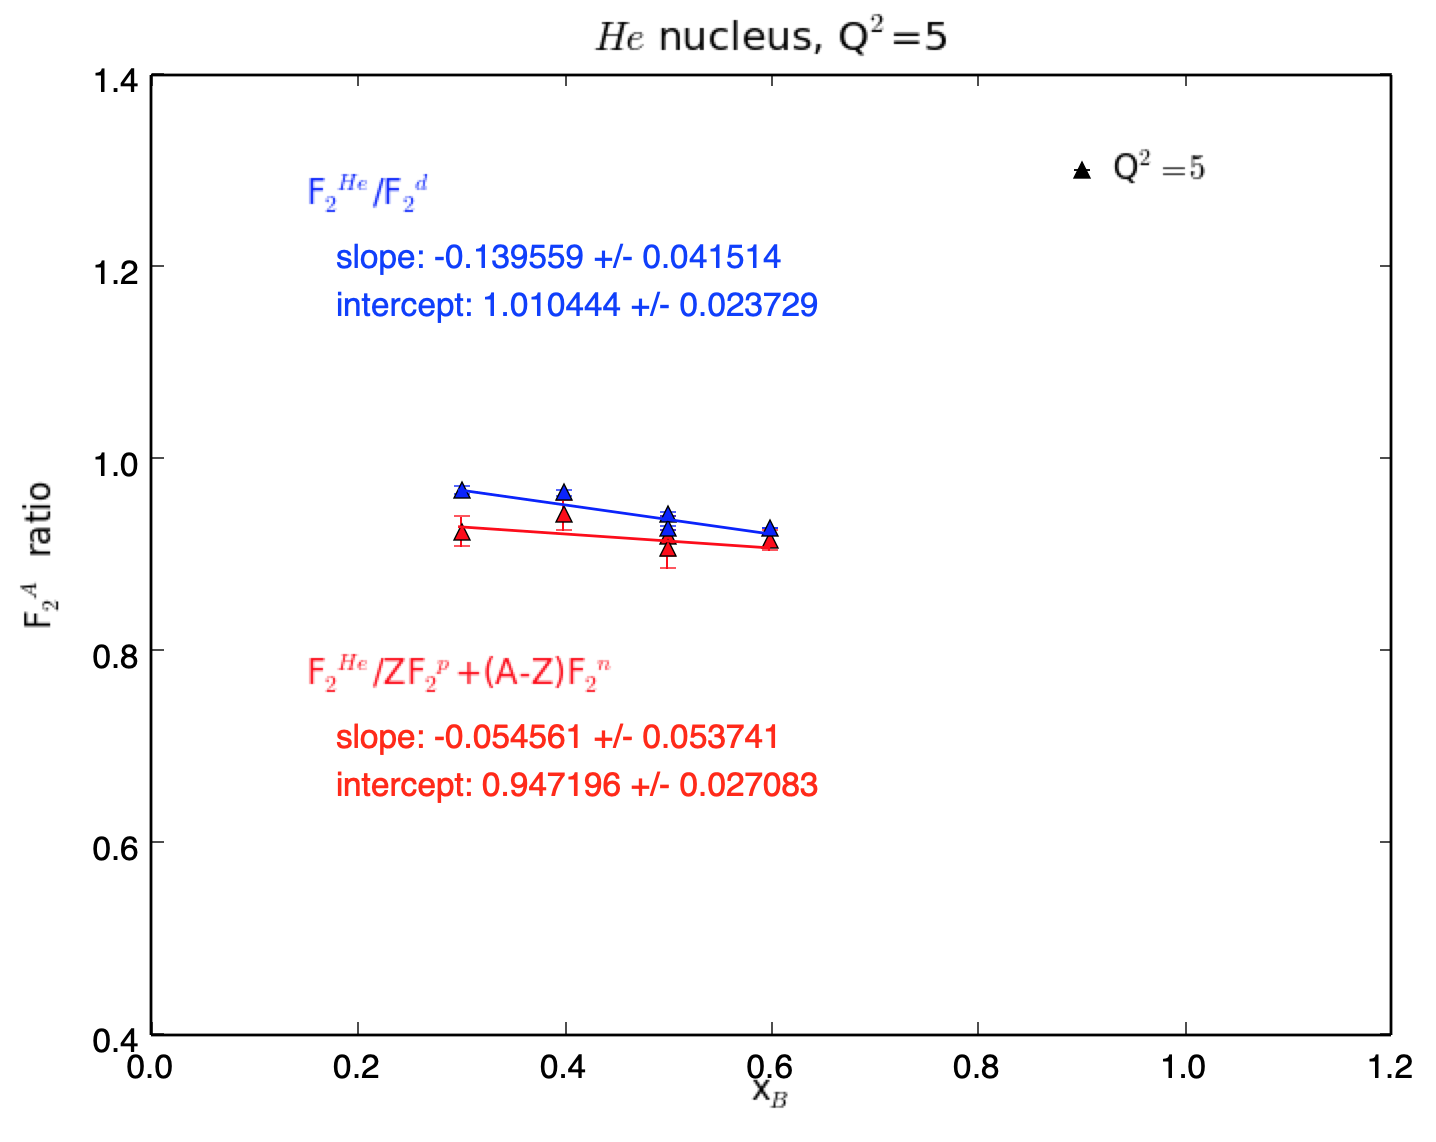
\includegraphics[width=\textwidth]{plots/q2_5/q2_5_He.png}
\end{minipage}\hfill\begin{minipage}{0.5\textwidth}
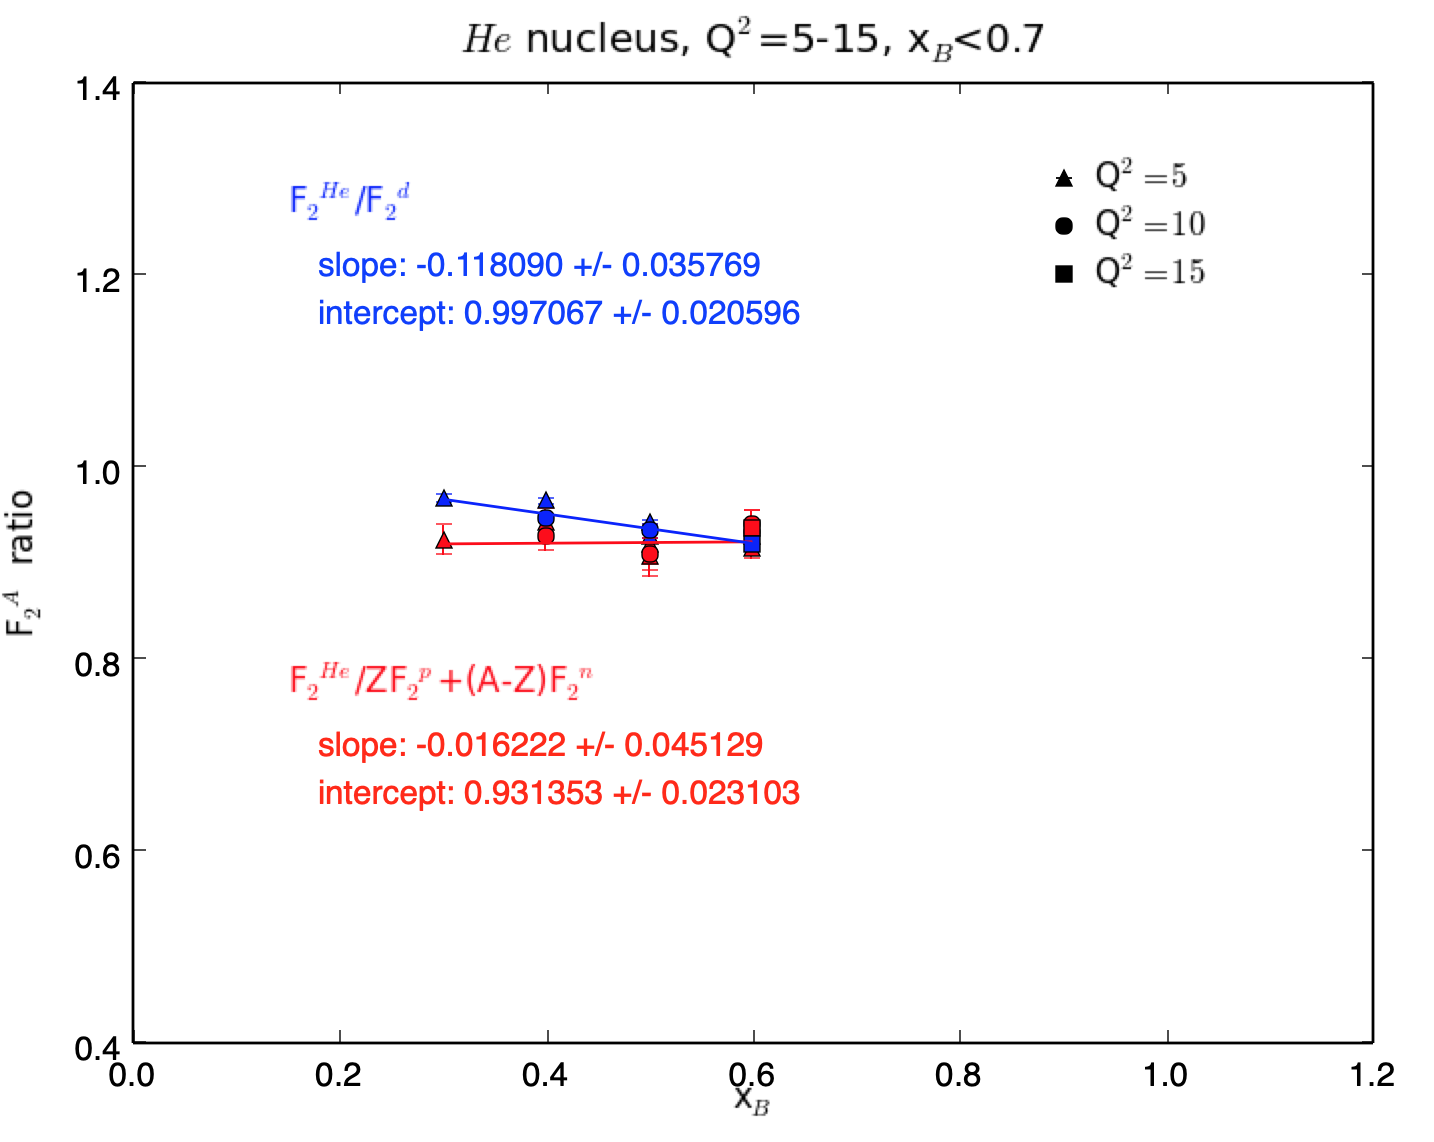
\includegraphics[width=\textwidth]{plots/q2_all_x_l7/q2_all_x_l7_He.png}
\end{minipage}\hfill\begin{minipage}{0.5\textwidth}
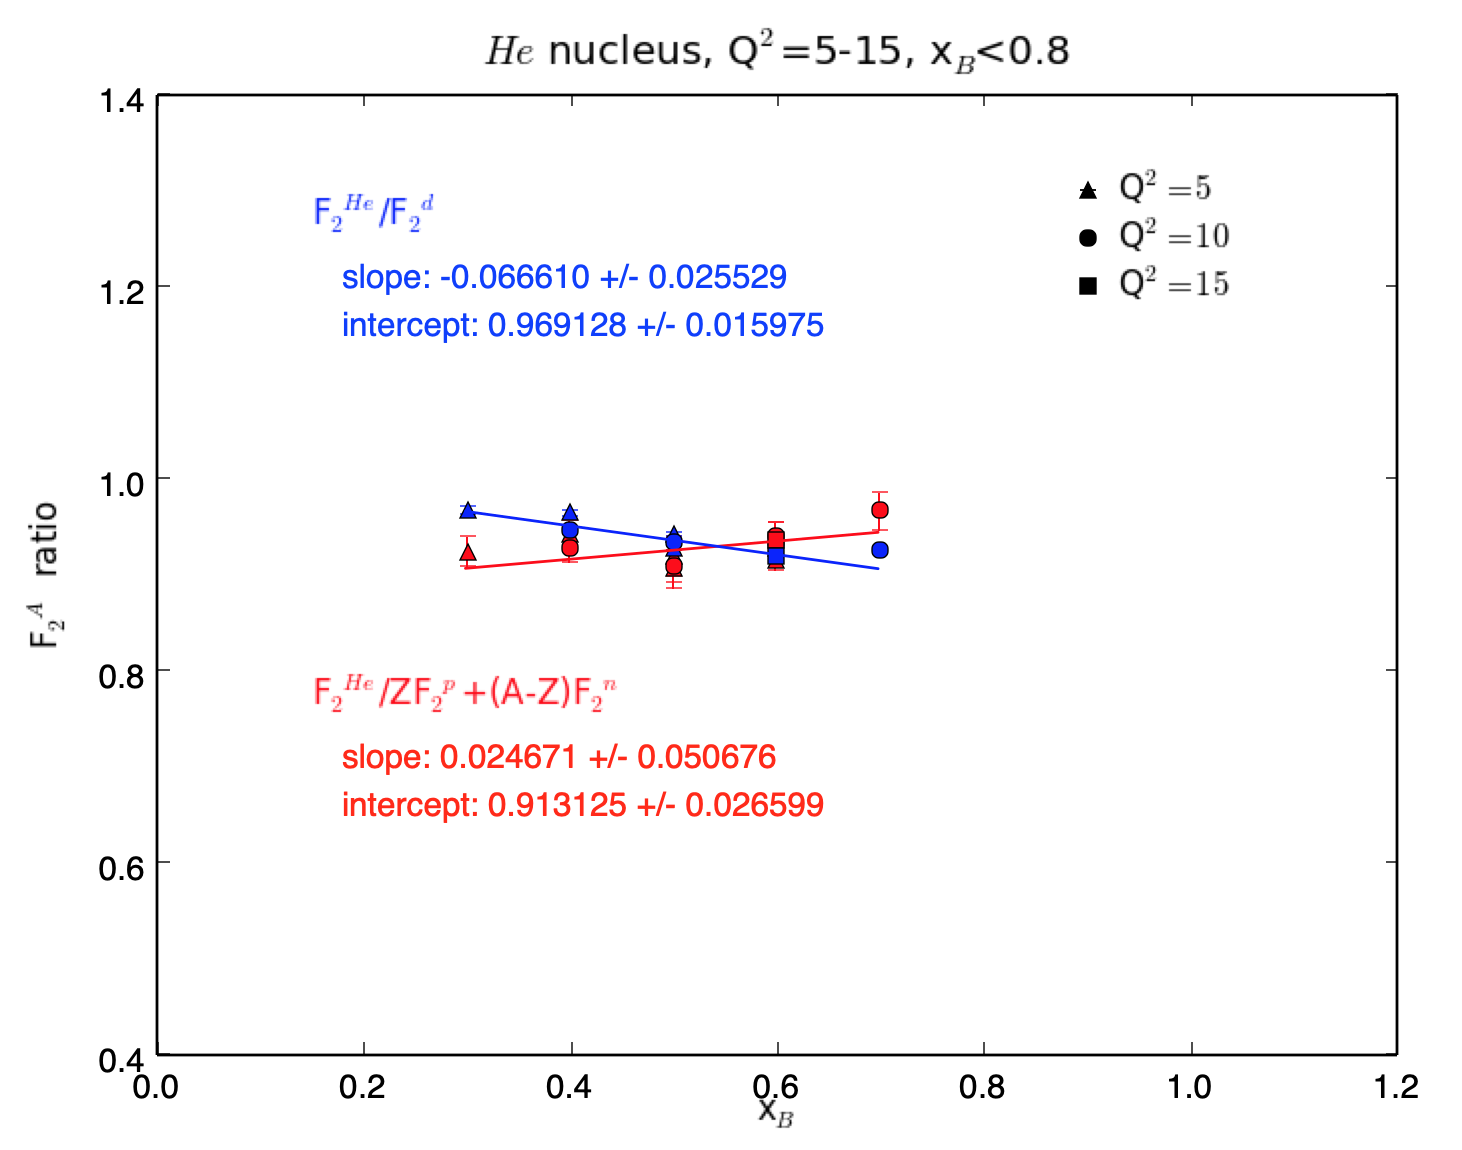
\includegraphics[width=\textwidth]{plots/q2_all_x_all/all_He.png}
\end{minipage}
  \caption[]{Linear fits to the $He$ target data with cuts on $Q^2$ and $x_B$.}
  \label{fig:fits_He}
\end{figure}   

 \begin{figure}[H]
\begin{minipage}{0.5\textwidth}
 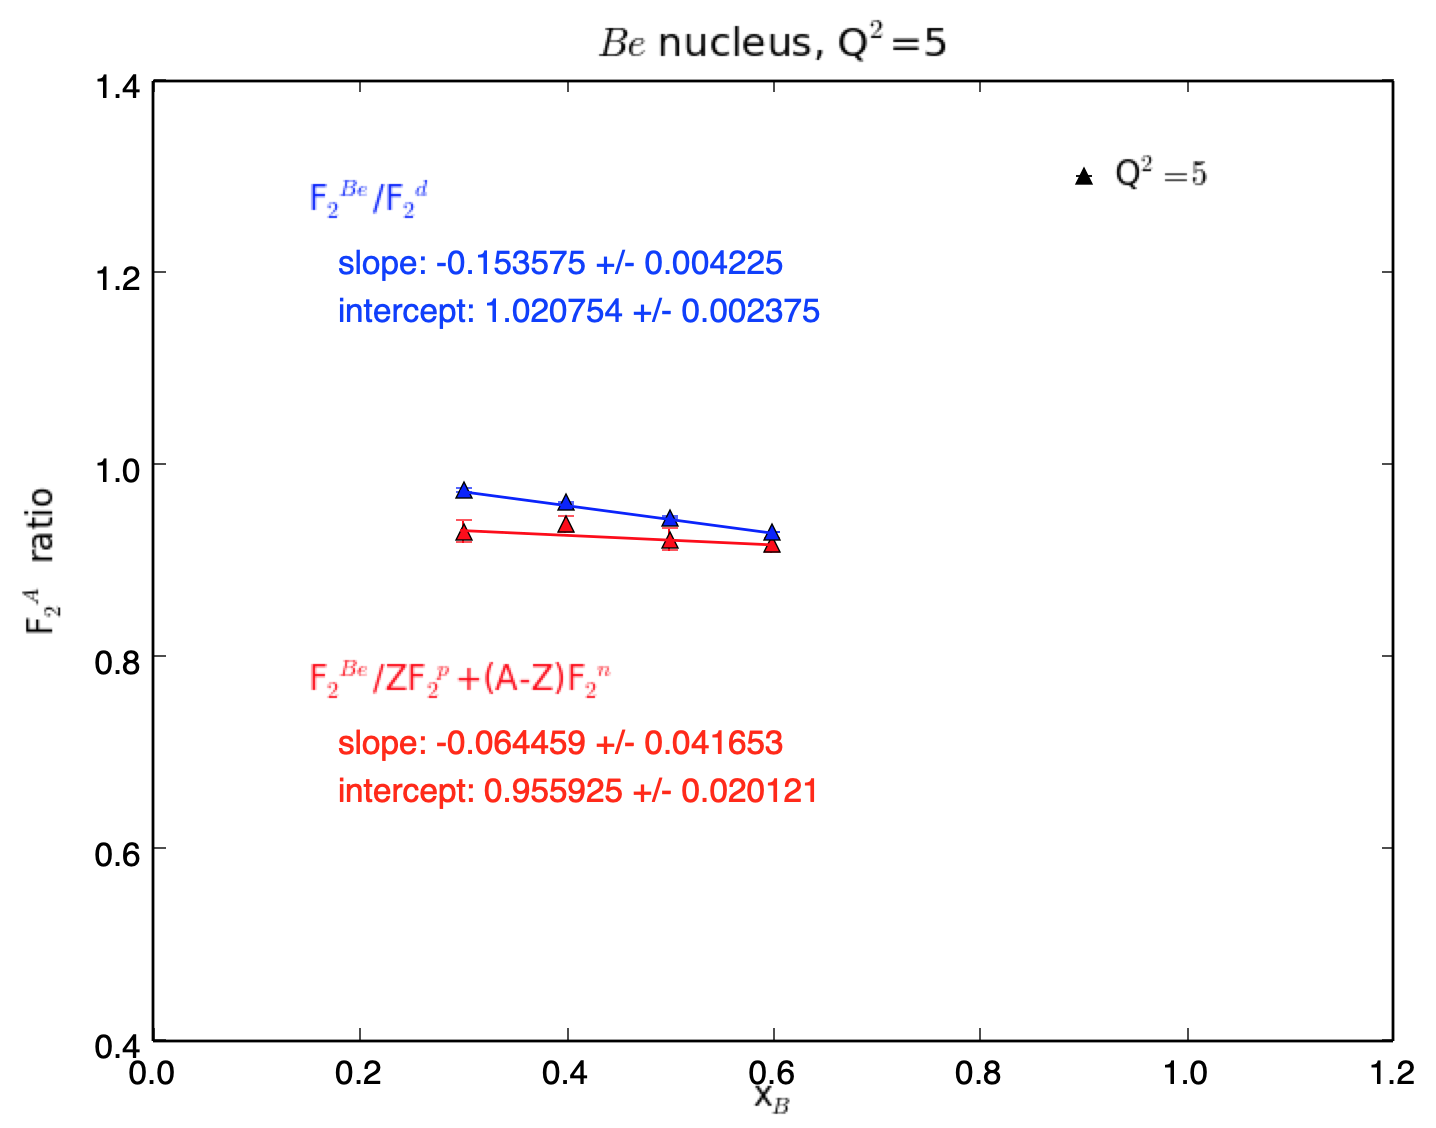
\includegraphics[width=\textwidth]{plots/q2_5/q2_5_Be.png}
\end{minipage}\hfill\begin{minipage}{0.5\textwidth}
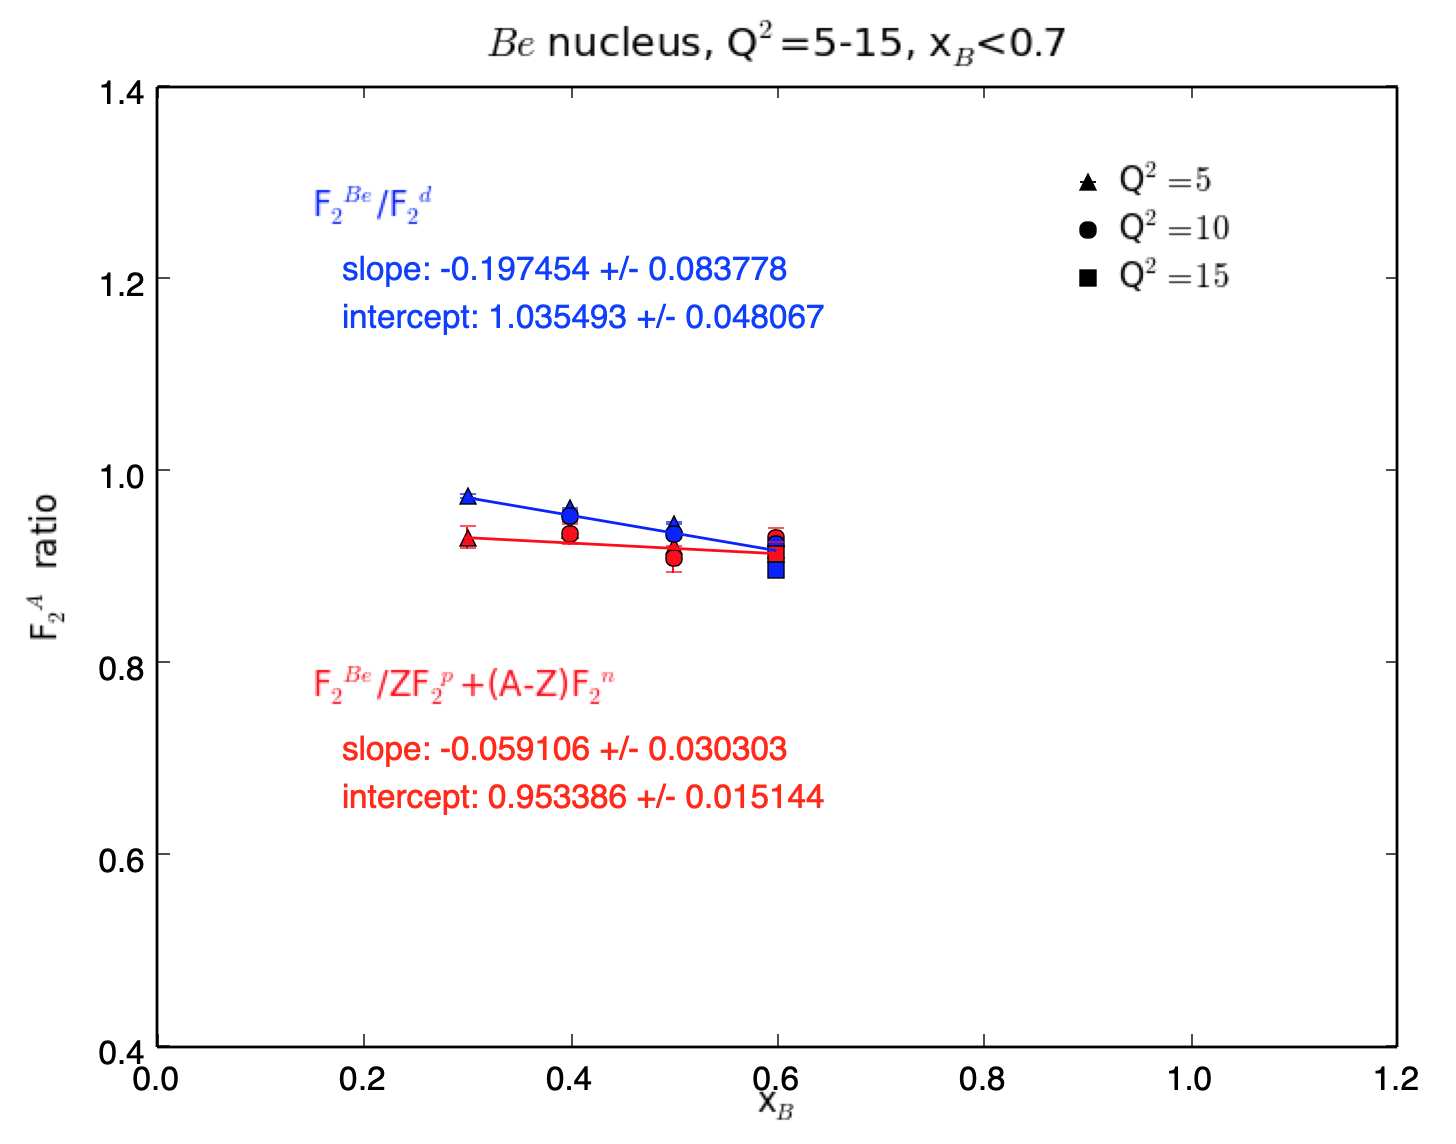
\includegraphics[width=\textwidth]{plots/q2_all_x_l7/q2_all_x_l7_Be.png}
\end{minipage}\hfill\begin{minipage}{0.5\textwidth}
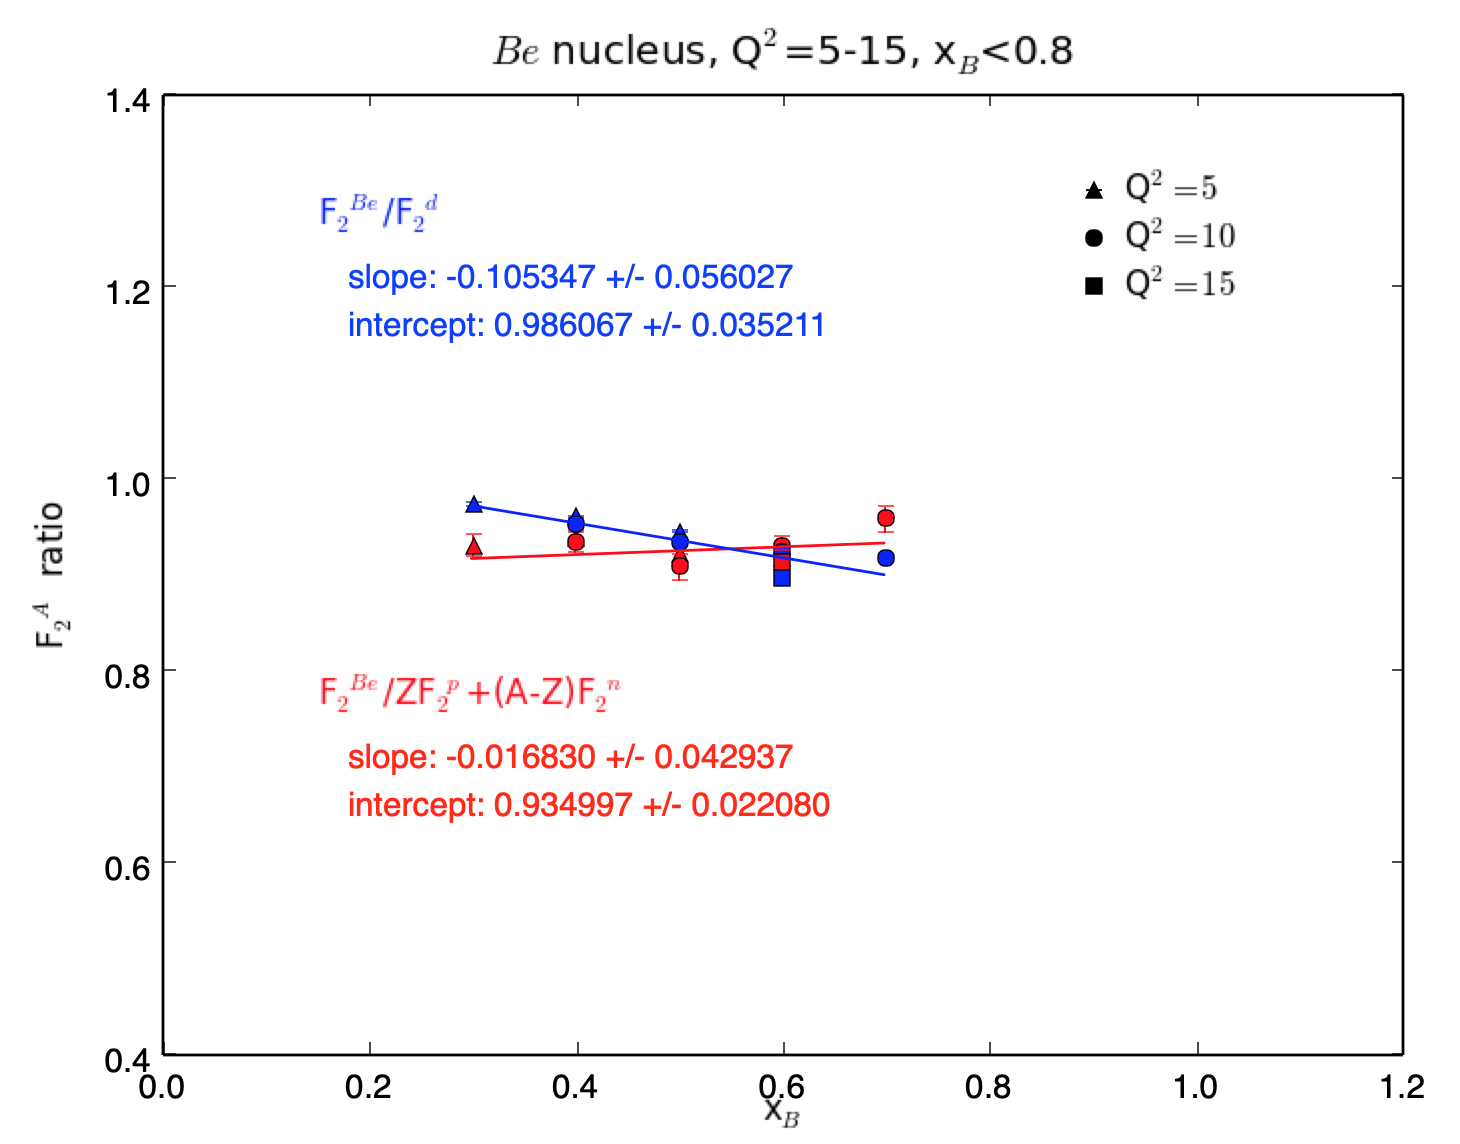
\includegraphics[width=\textwidth]{plots/q2_all_x_all/all_Be.png}
\end{minipage}
  \caption[]{Linear fits to the $Be$ target data with cuts on $Q^2$ and $x_B$.}
  \label{fig:fits_Be}
\end{figure}   


 \begin{figure}[H]
\begin{minipage}{0.5\textwidth}
 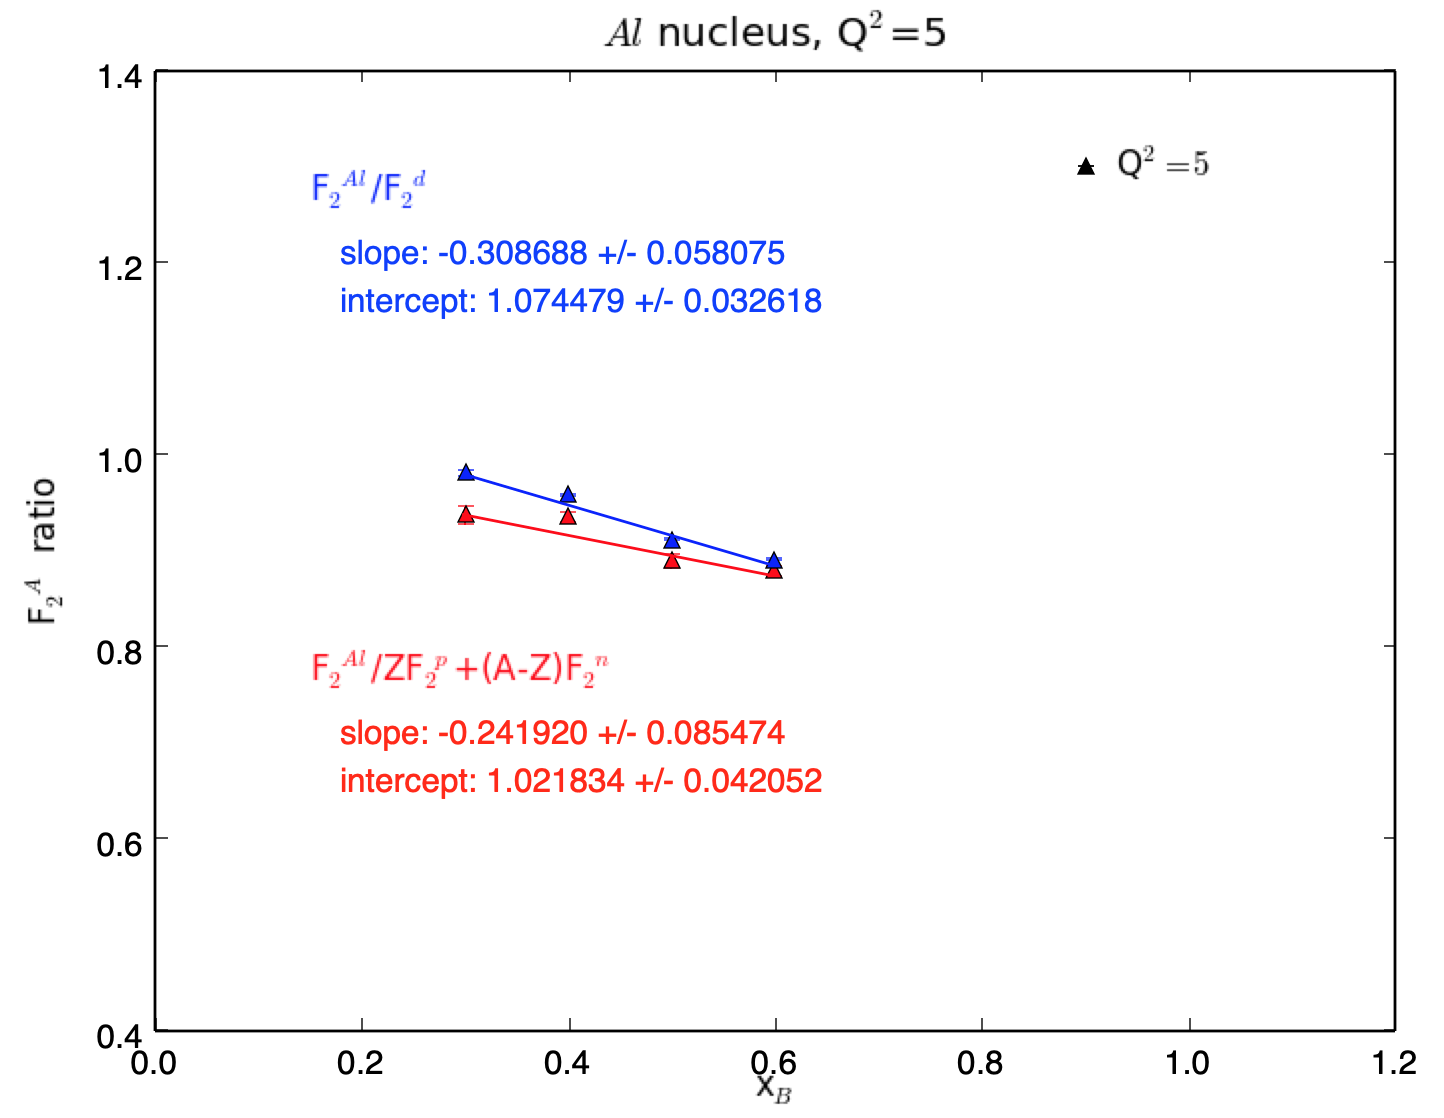
\includegraphics[width=\textwidth]{plots/q2_5/q2_5_Al.png}
\end{minipage}\hfill\begin{minipage}{0.5\textwidth}
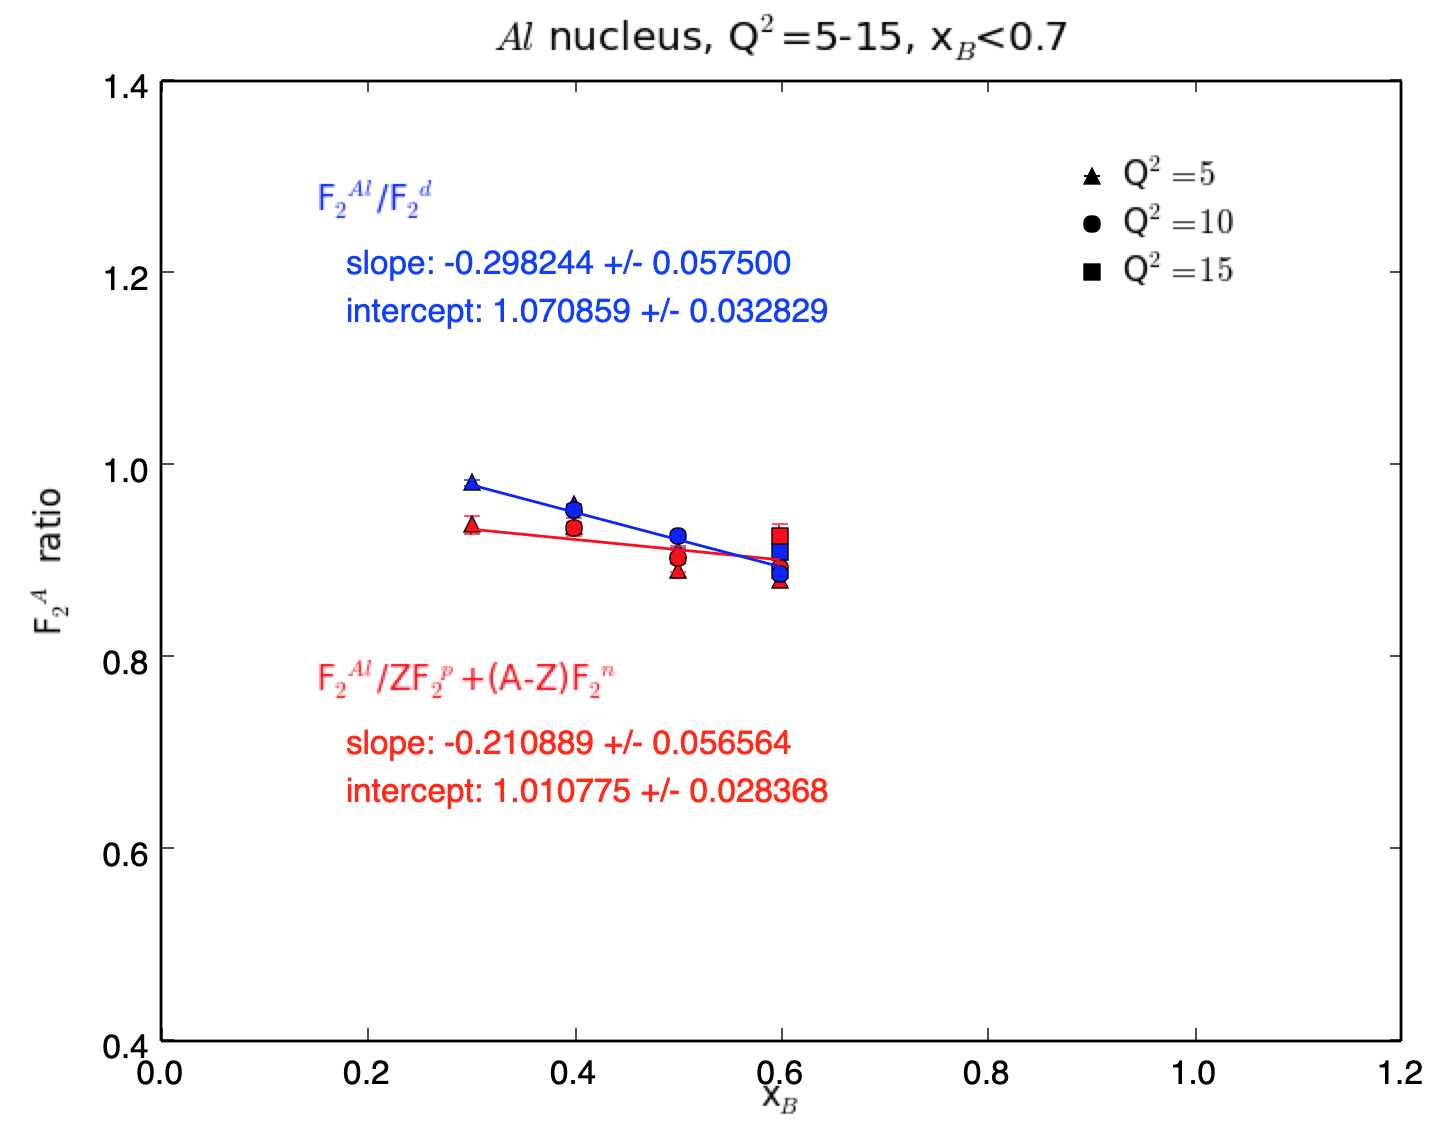
\includegraphics[width=\textwidth]{plots/q2_all_x_l7/q2_all_x_l7_Al.png}
\end{minipage}\hfill\begin{minipage}{0.5\textwidth}
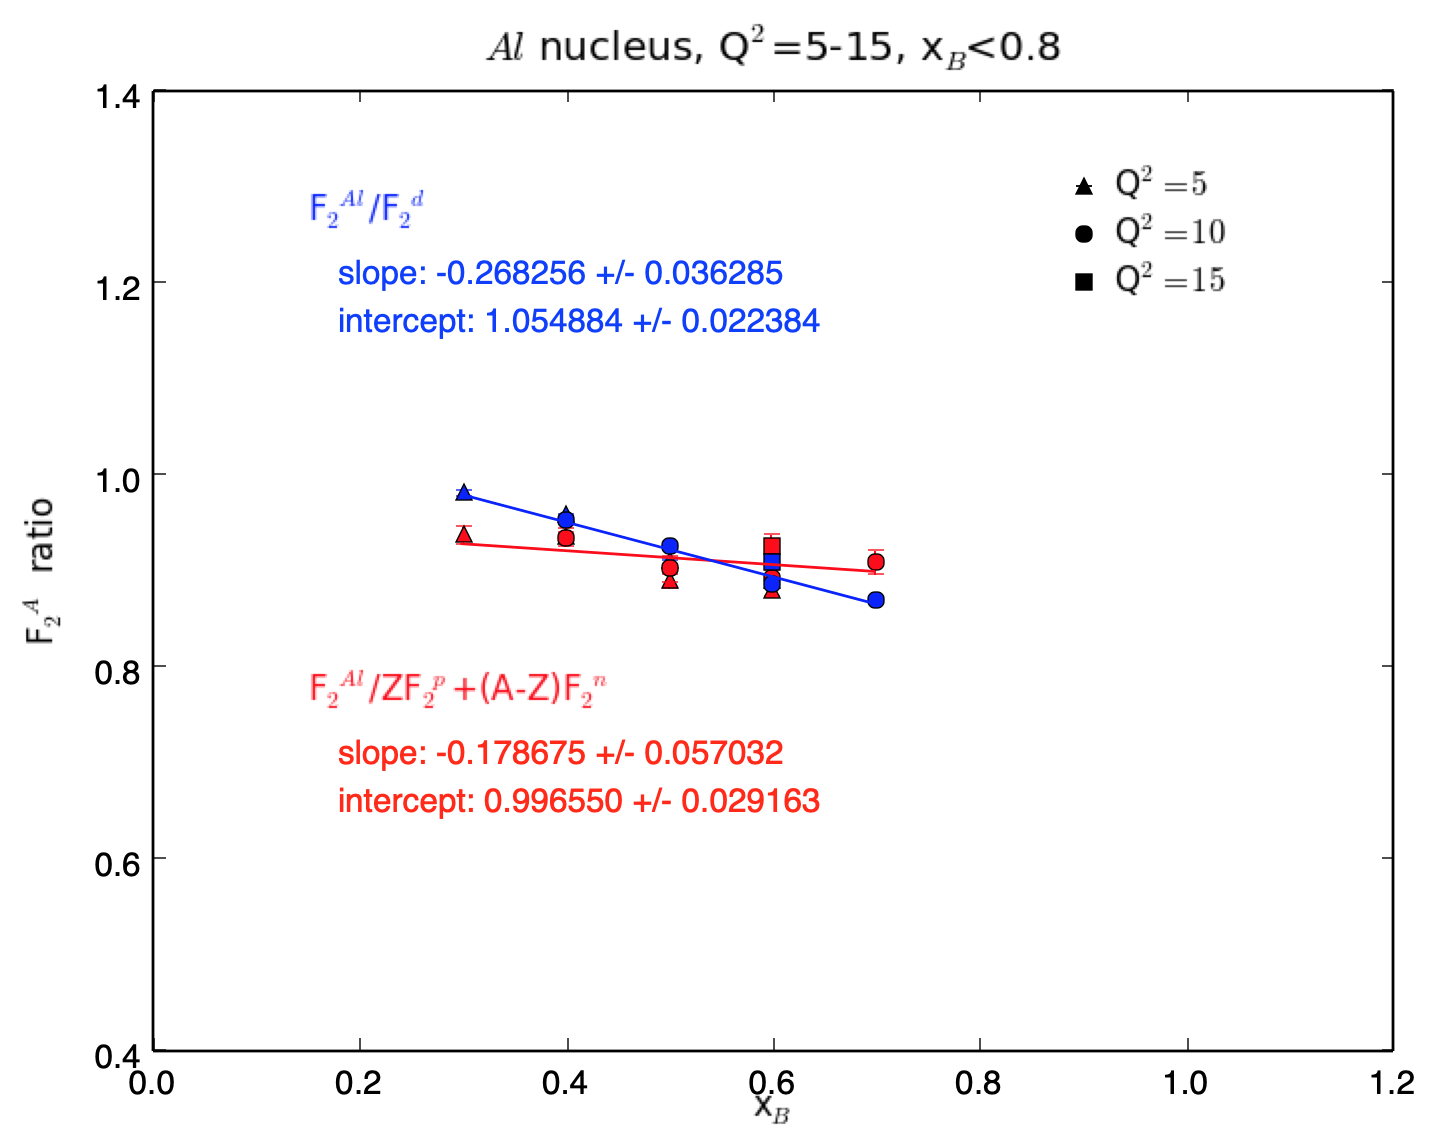
\includegraphics[width=\textwidth]{plots/q2_all_x_all/all_Al.png}
\end{minipage}
  \caption[]{Linear fits to the $Al$ target data with cuts on $Q^2$ and $x_B$.}
  \label{fig:fits_Al}
\end{figure}   


 \begin{figure}[H]
\begin{minipage}{0.5\textwidth}
 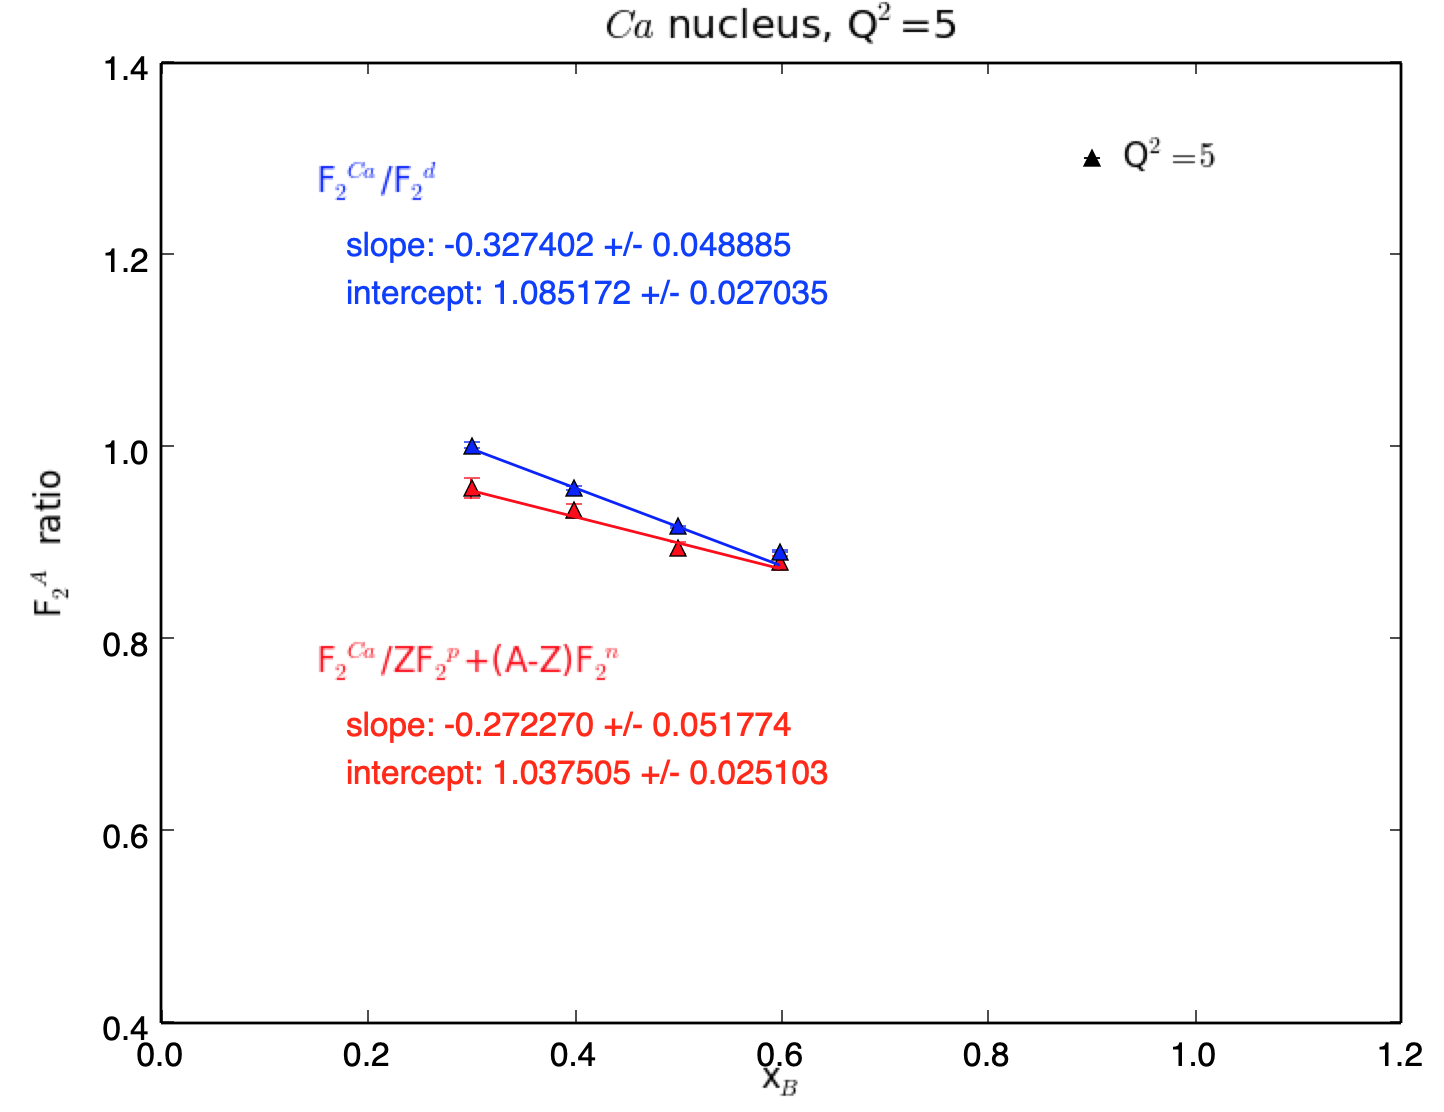
\includegraphics[width=\textwidth]{plots/q2_5/q2_5_Ca.png}
\end{minipage}\hfill\begin{minipage}{0.5\textwidth}
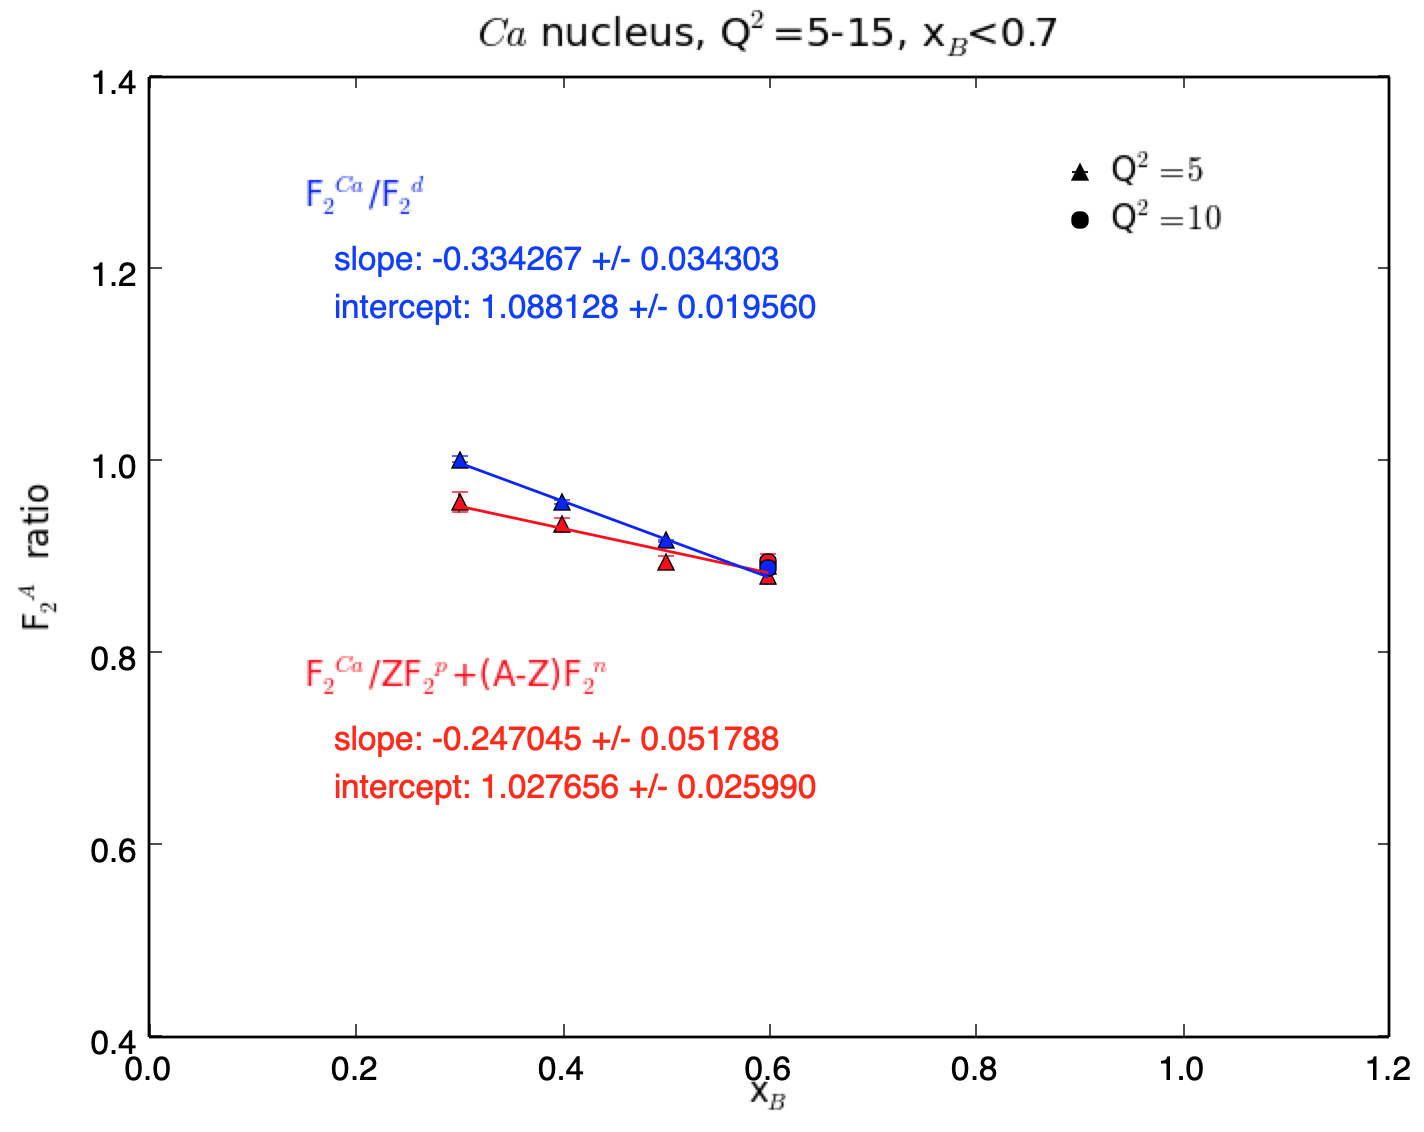
\includegraphics[width=\textwidth]{plots/q2_all_x_l7/q2_all_x_l7_Ca.png}
\end{minipage}\hfill\begin{minipage}{0.5\textwidth}
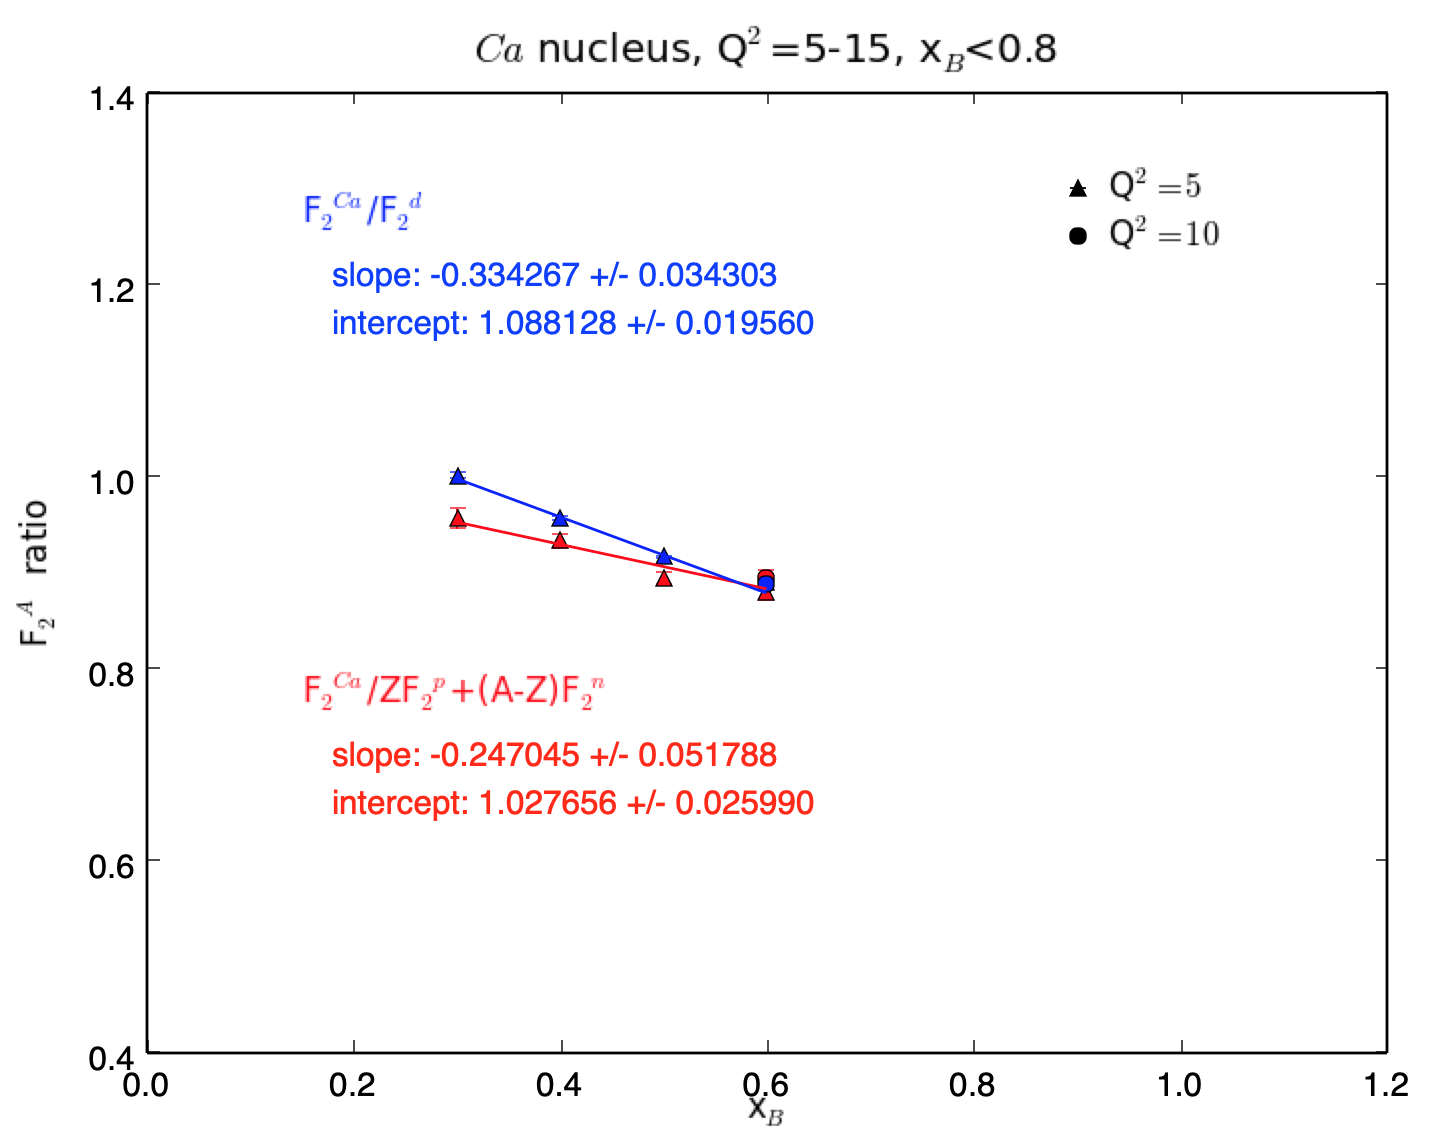
\includegraphics[width=\textwidth]{plots/q2_all_x_all/all_Ca.png}
\end{minipage}
  \caption[]{Linear fits to the $Ca$ target data with cuts on $Q^2$ and $x_B$.}
  \label{fig:fits_Ca}
\end{figure}   

 \begin{figure}[H]
\begin{minipage}{0.5\textwidth}
 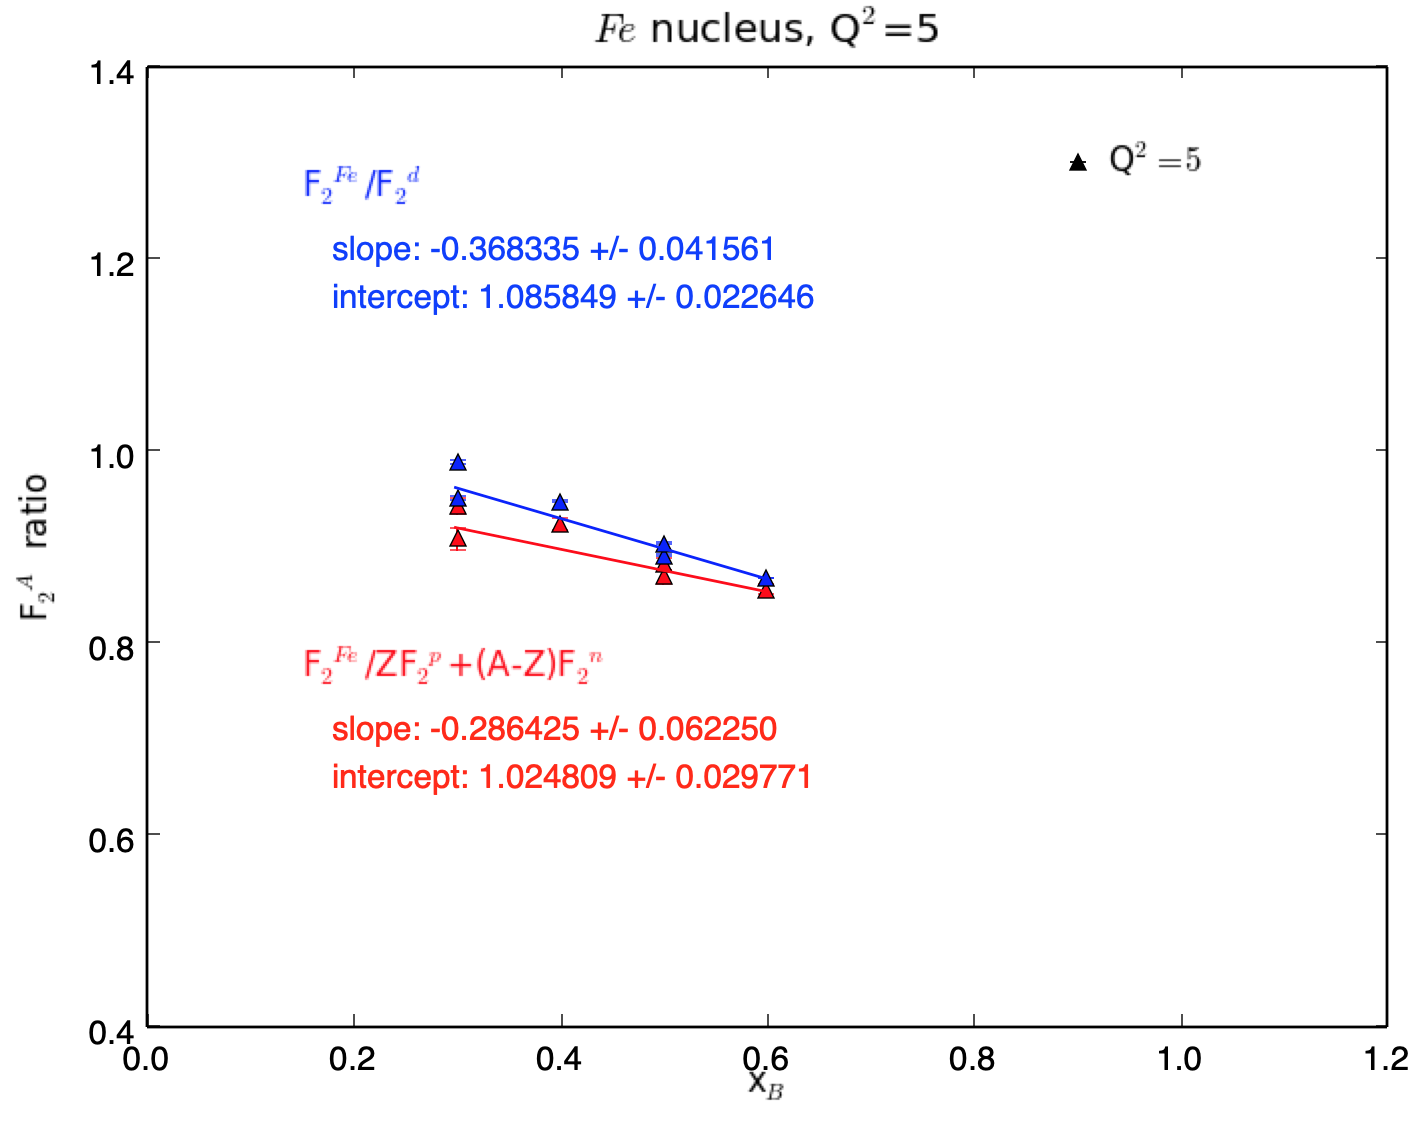
\includegraphics[width=\textwidth]{plots/q2_5/q2_5_Fe.png}
\end{minipage}\hfill\begin{minipage}{0.5\textwidth}
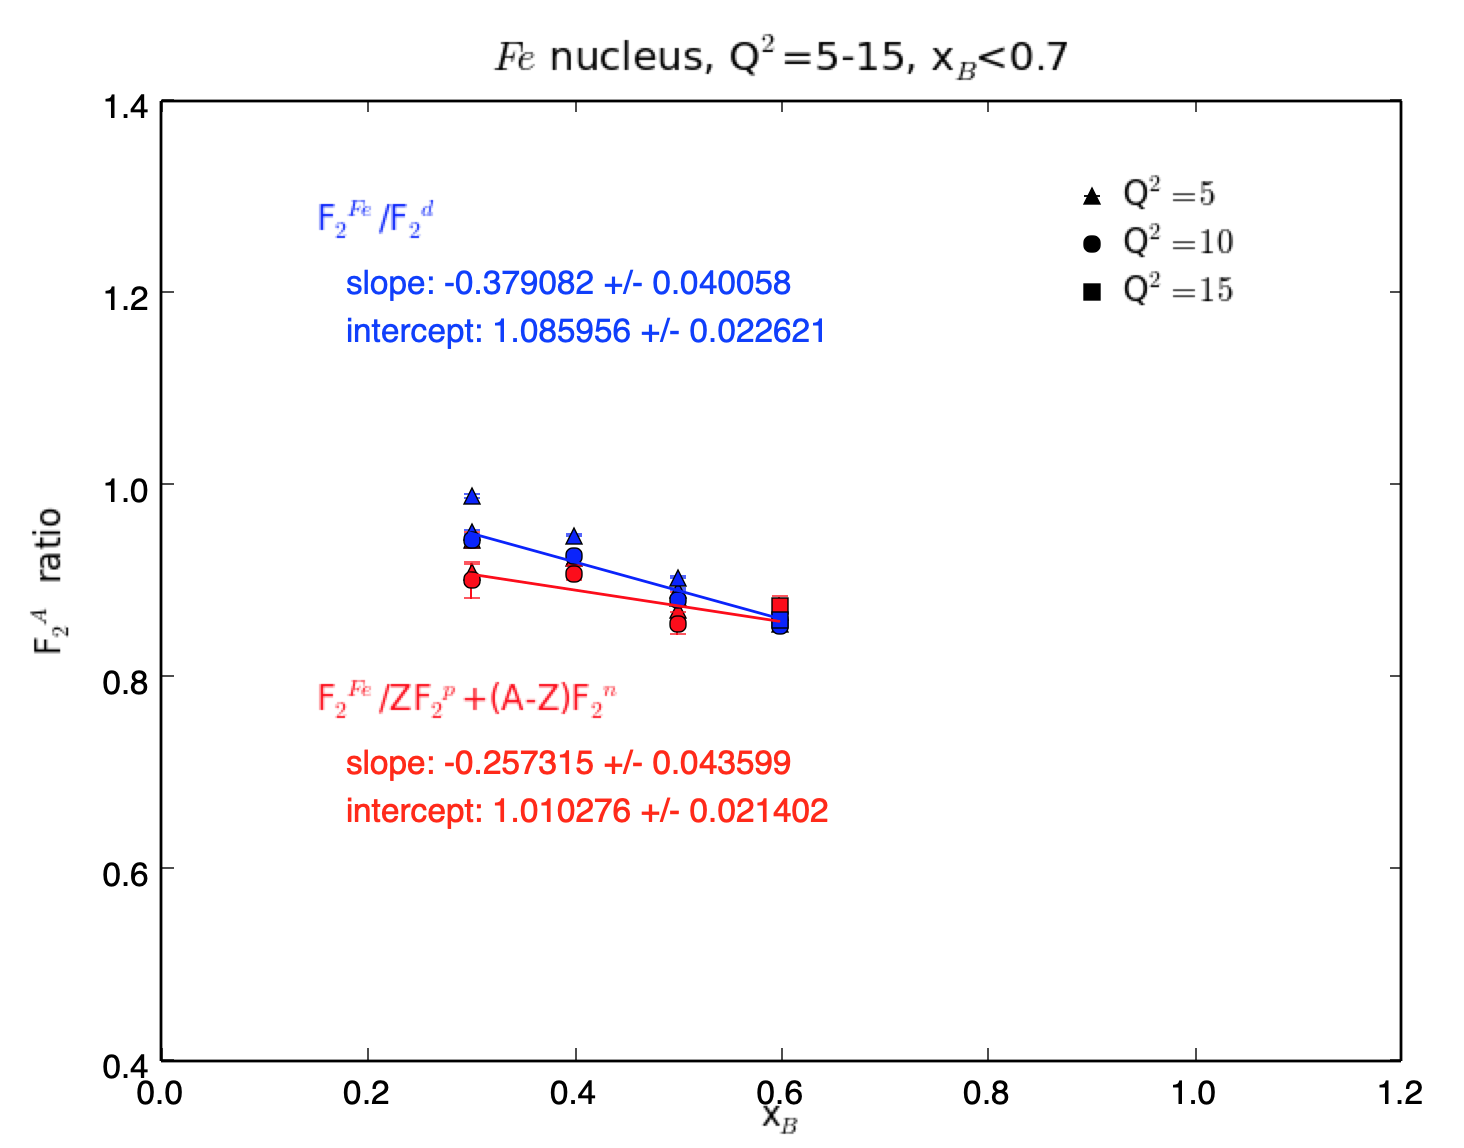
\includegraphics[width=\textwidth]{plots/q2_all_x_l7/q2_all_x_l7_Fe.png}
\end{minipage}\hfill\begin{minipage}{0.5\textwidth}
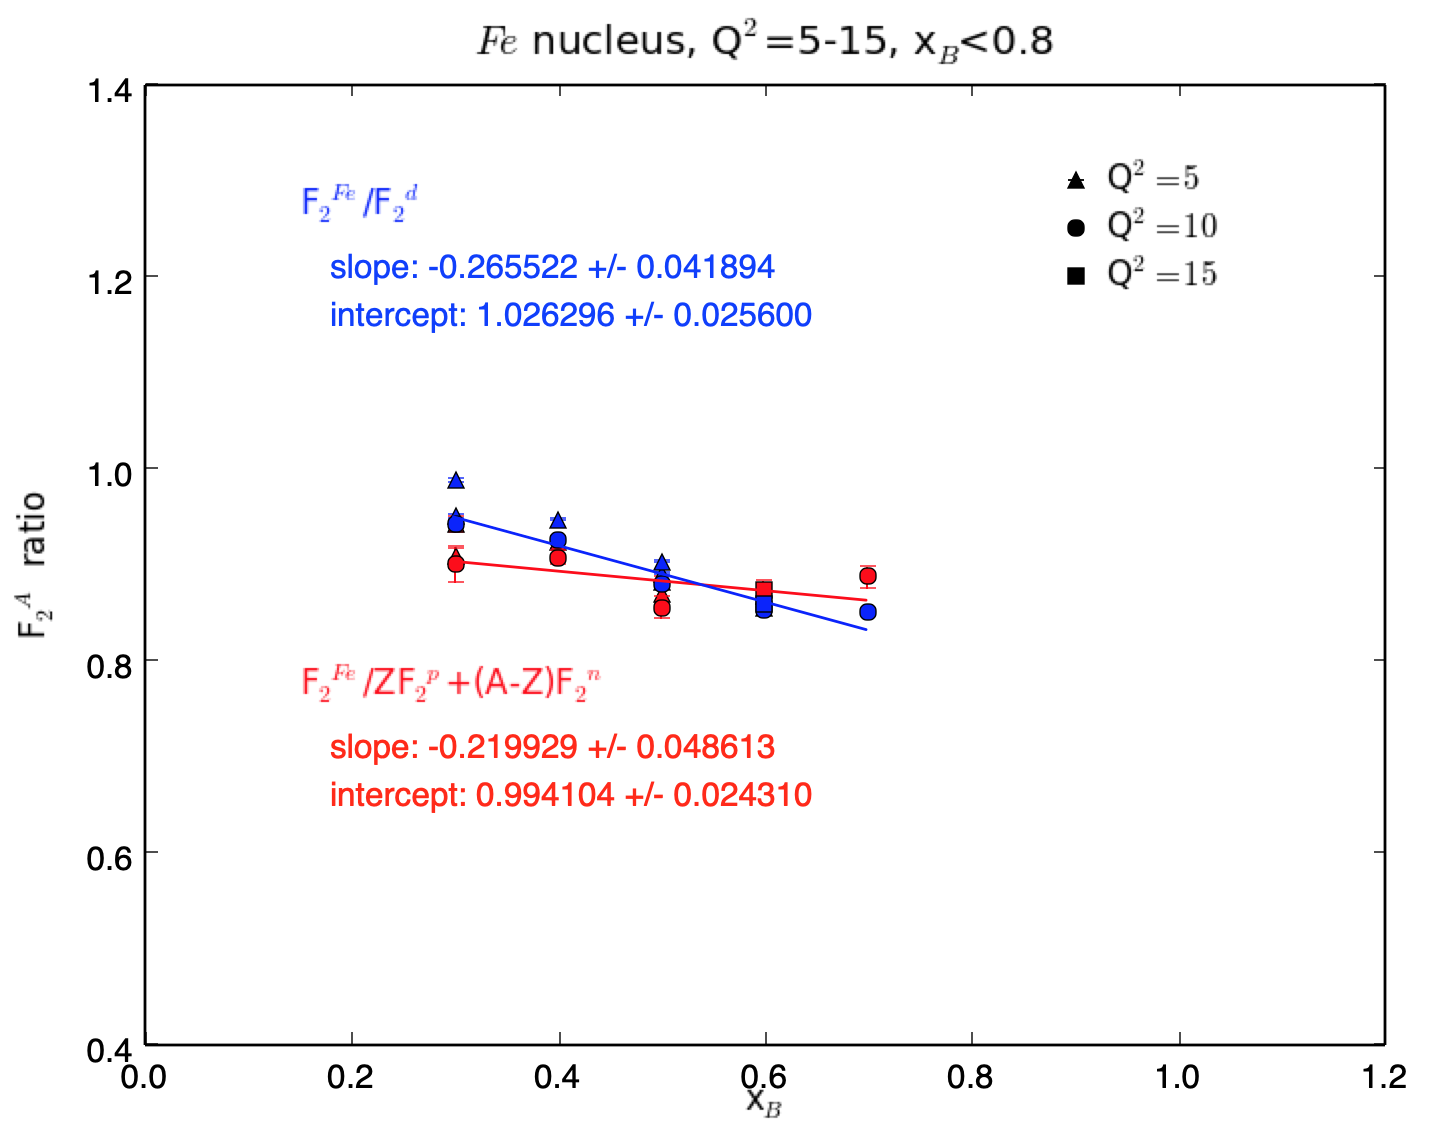
\includegraphics[width=\textwidth]{plots/q2_all_x_all/all_Fe.png}
\end{minipage}
  \caption[]{Linear fits to the $Fe$ target data with cuts on $Q^2$ and $x_B$.}
  \label{fig:fits_Fe}
\end{figure}   

 \begin{figure}[H]
\begin{minipage}{0.5\textwidth}
 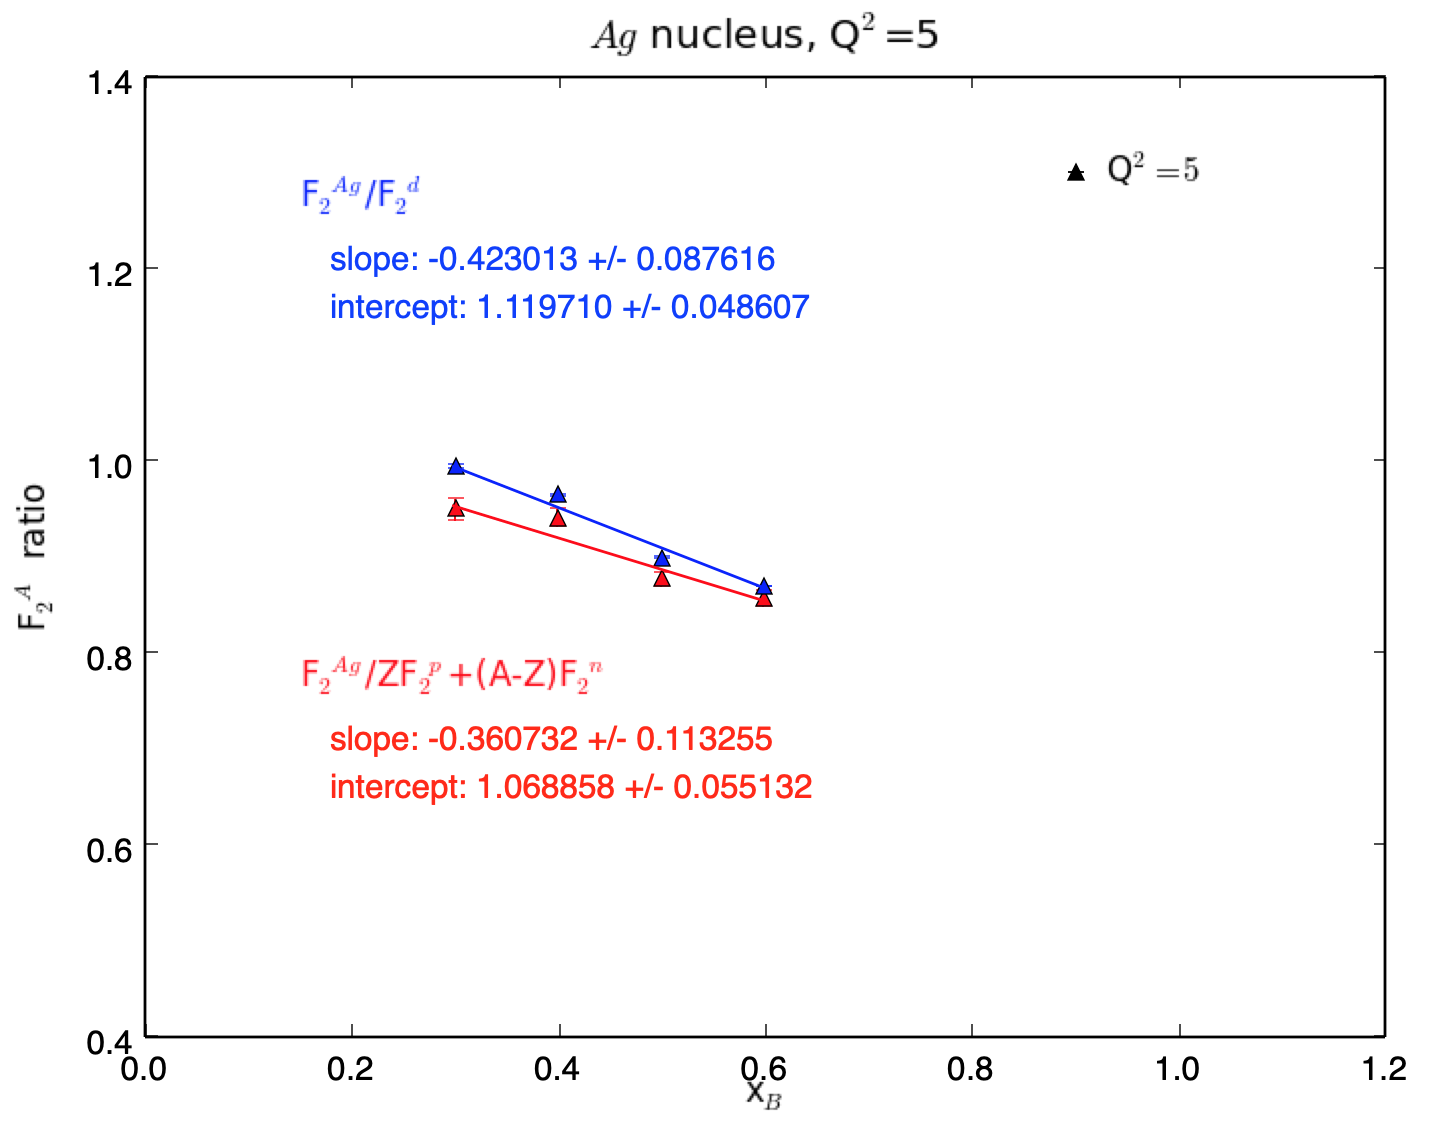
\includegraphics[width=\textwidth]{plots/q2_5/q2_5_Ag.png}
\end{minipage}\hfill\begin{minipage}{0.5\textwidth}
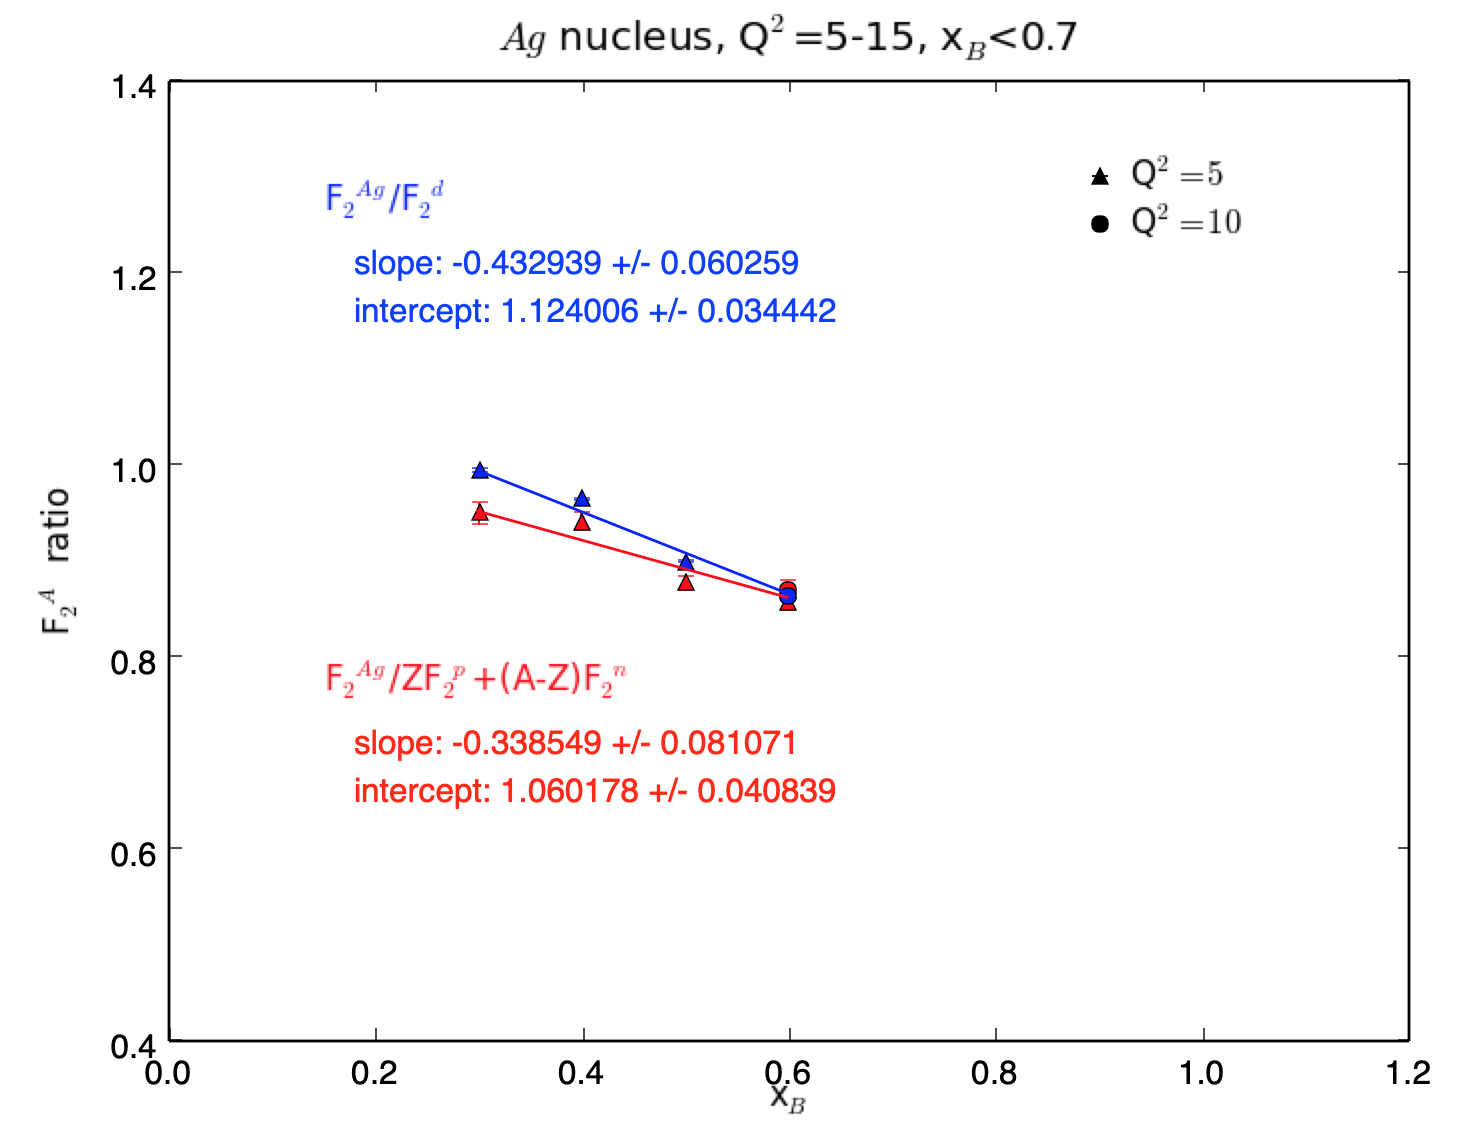
\includegraphics[width=\textwidth]{plots/q2_all_x_l7/q2_all_x_l7_Ag.png}
\end{minipage}\hfill\begin{minipage}{0.5\textwidth}
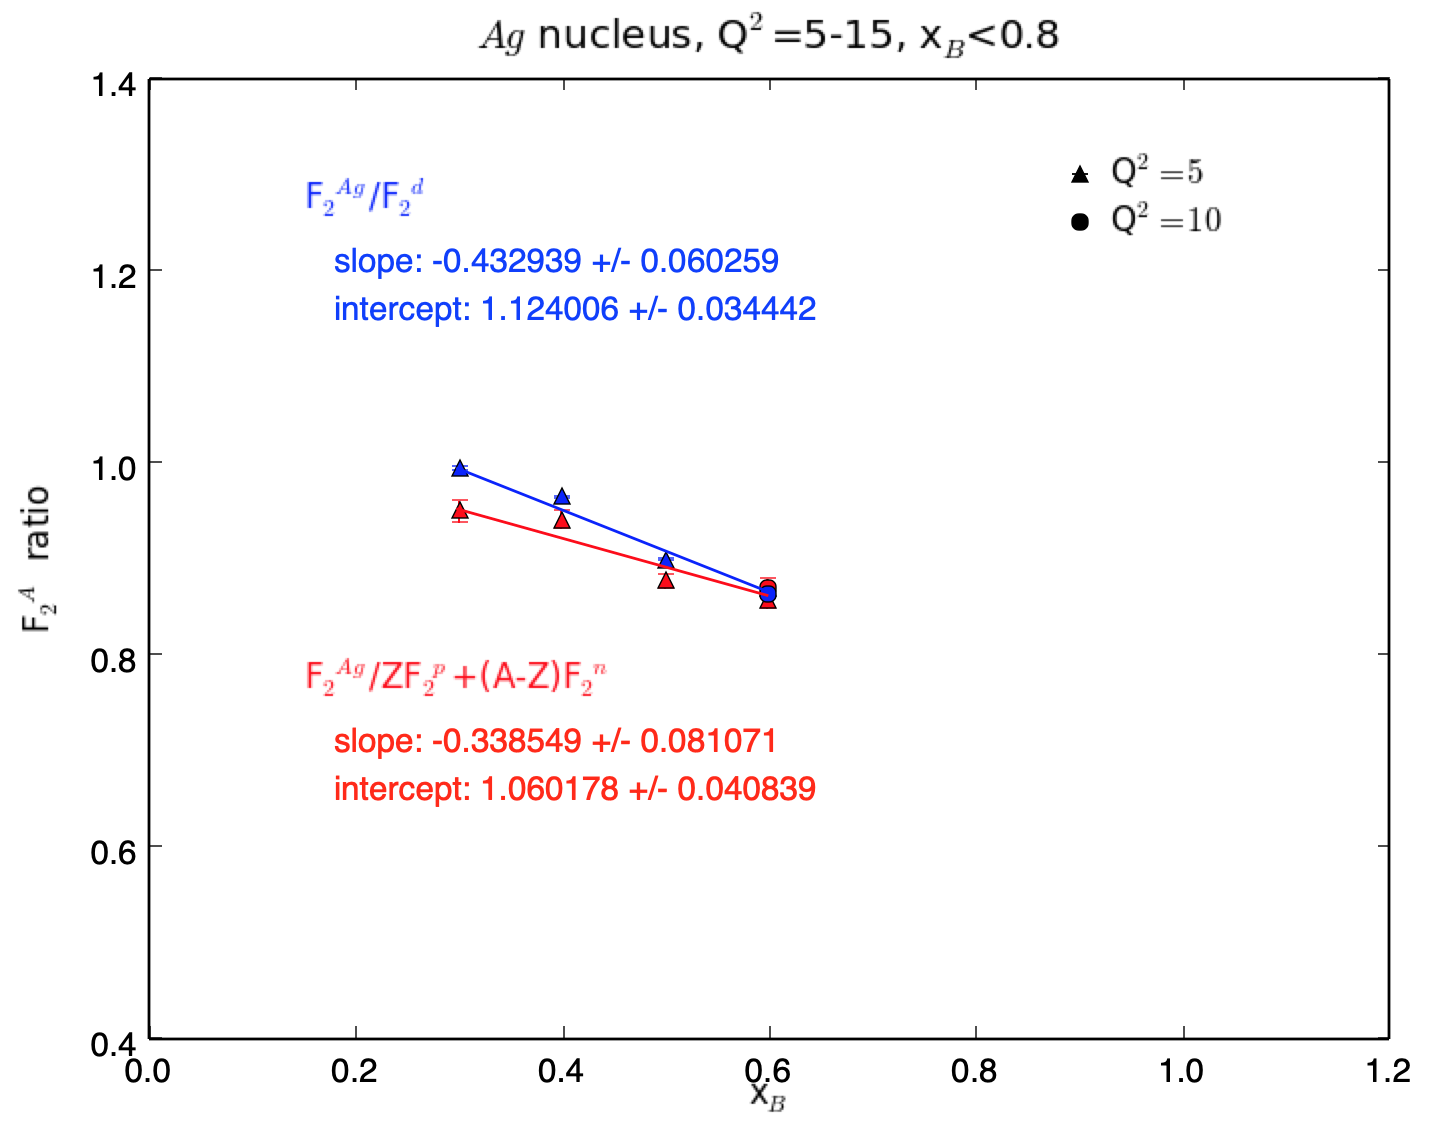
\includegraphics[width=\textwidth]{plots/q2_all_x_all/all_Ag.png}
\end{minipage}
  \caption[]{Linear fits to the $Ag$ target data with cuts on $Q^2$ and $x_B$.}
  \label{fig:fits_Ag}
\end{figure}   

\begin{figure}[H]
\begin{minipage}{0.5\textwidth}
      	  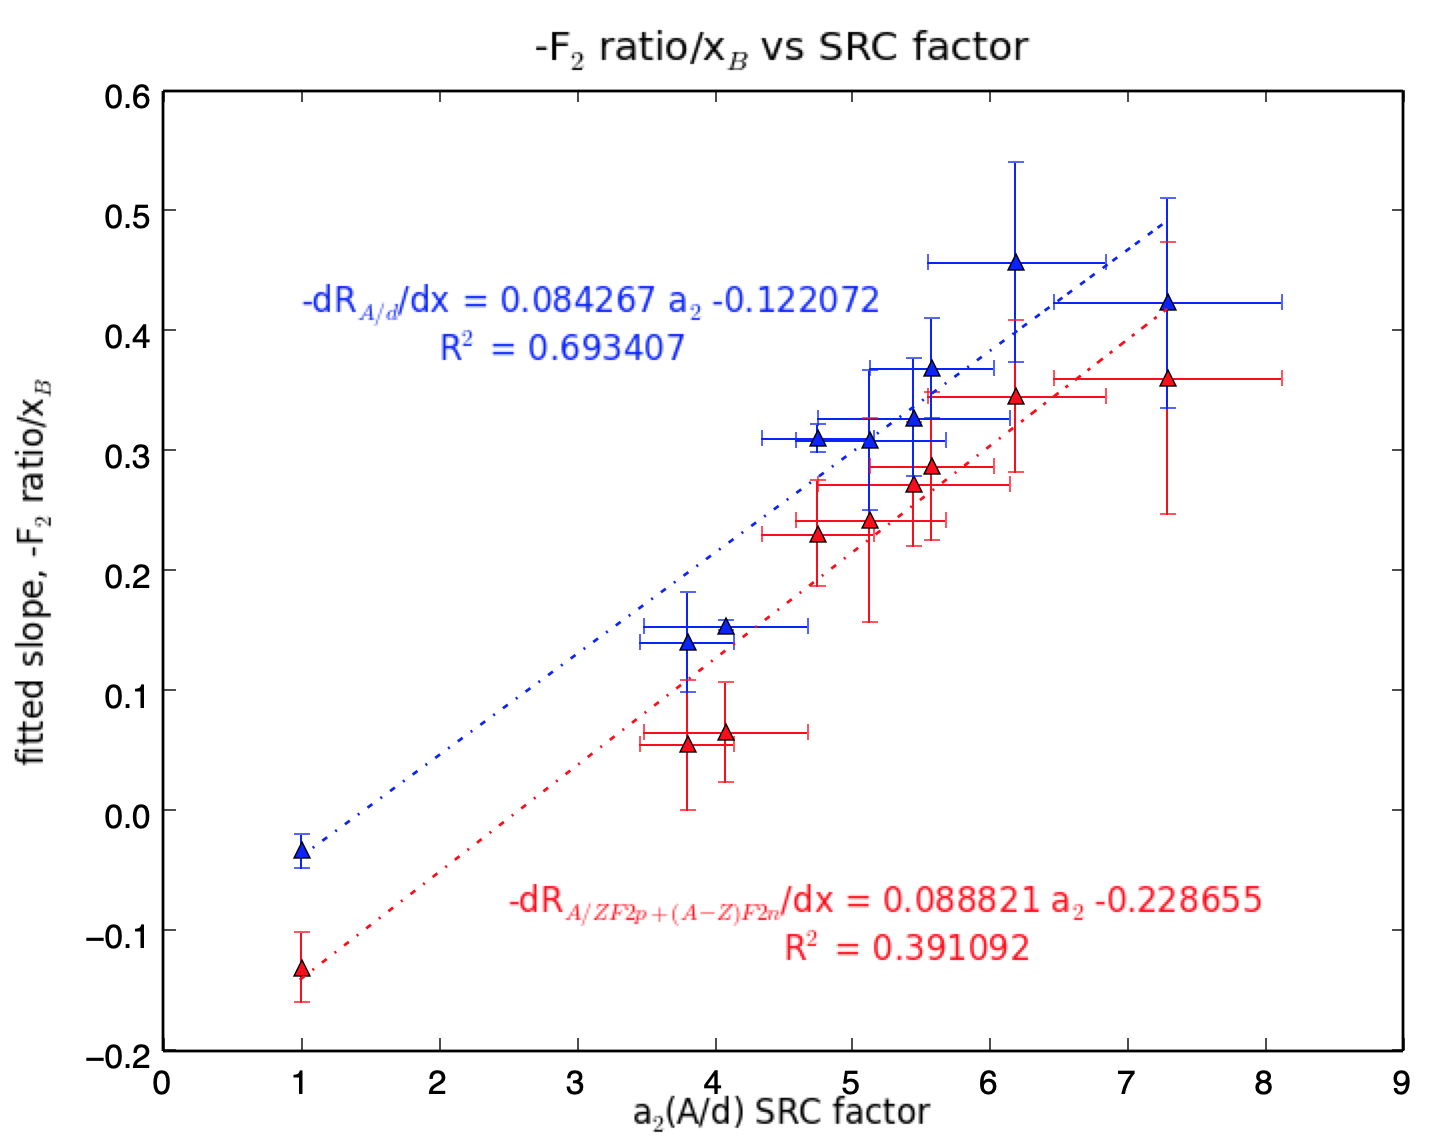
\includegraphics[width=\textwidth]{plots/a2SRC.png}
      	  \end{minipage}\hfill\begin{minipage}{0.5\textwidth}
      	        	  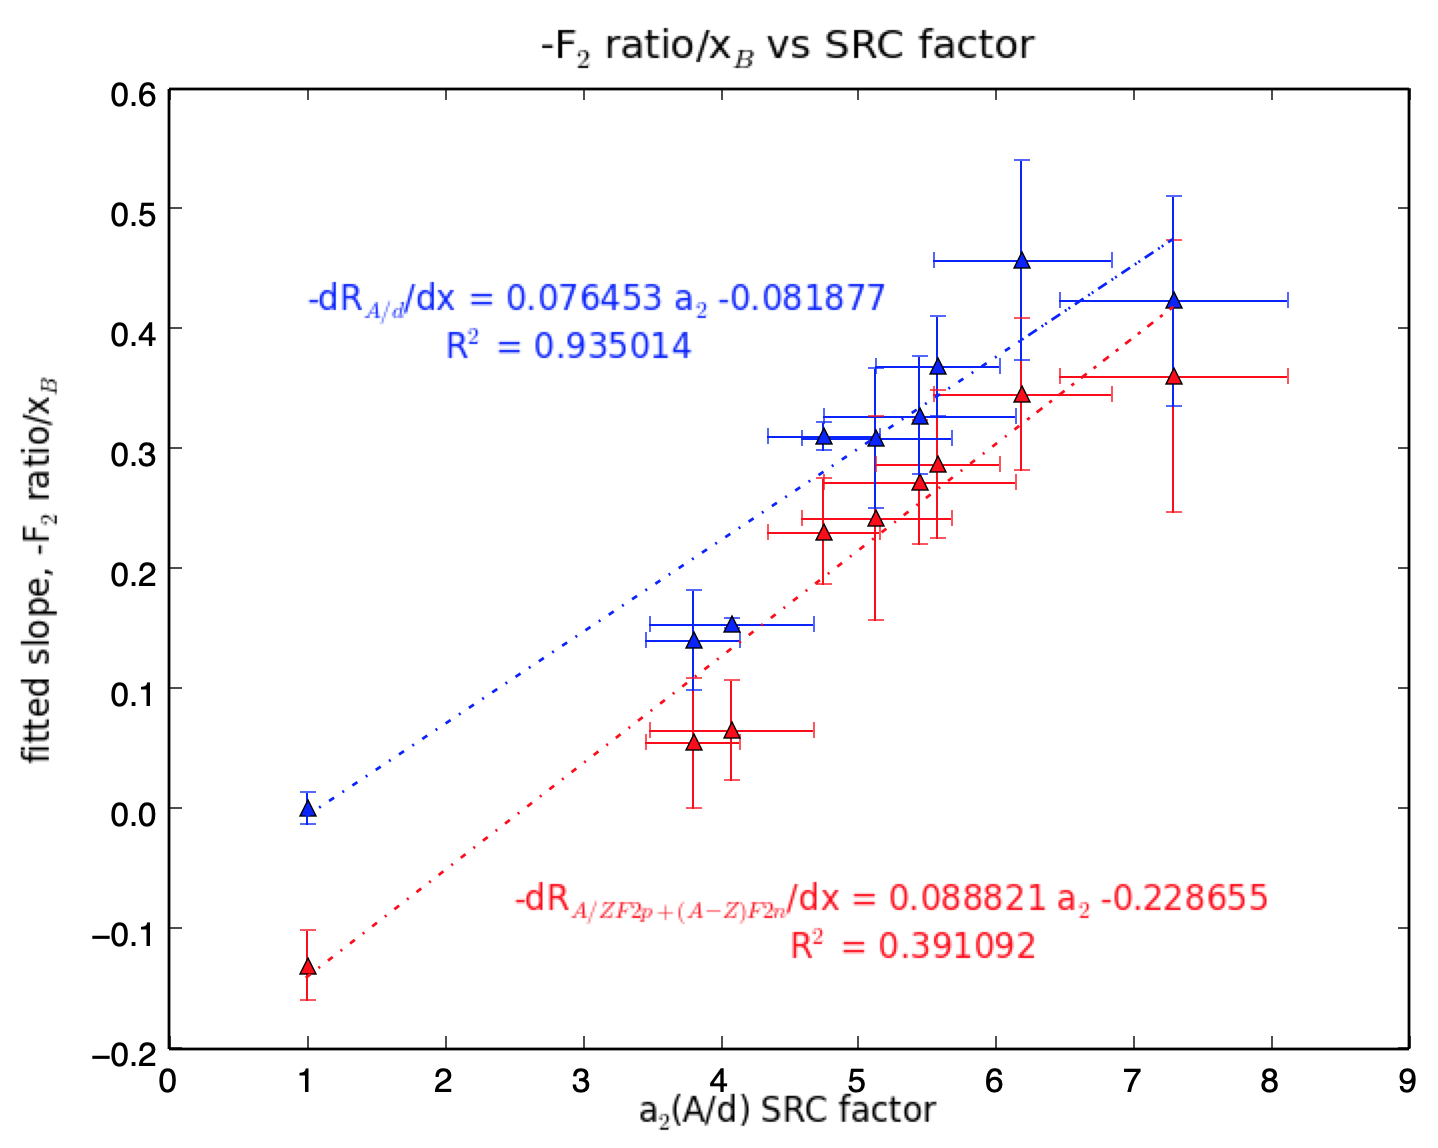
\includegraphics[width=\textwidth]{plots/a2SRCfixed.png}
\end{minipage}
 	 \caption[]{}
  \label{fig:a2_src}
 \end{figure}
 
  \begin{figure}[H]
\begin{minipage}{0.5\textwidth}
 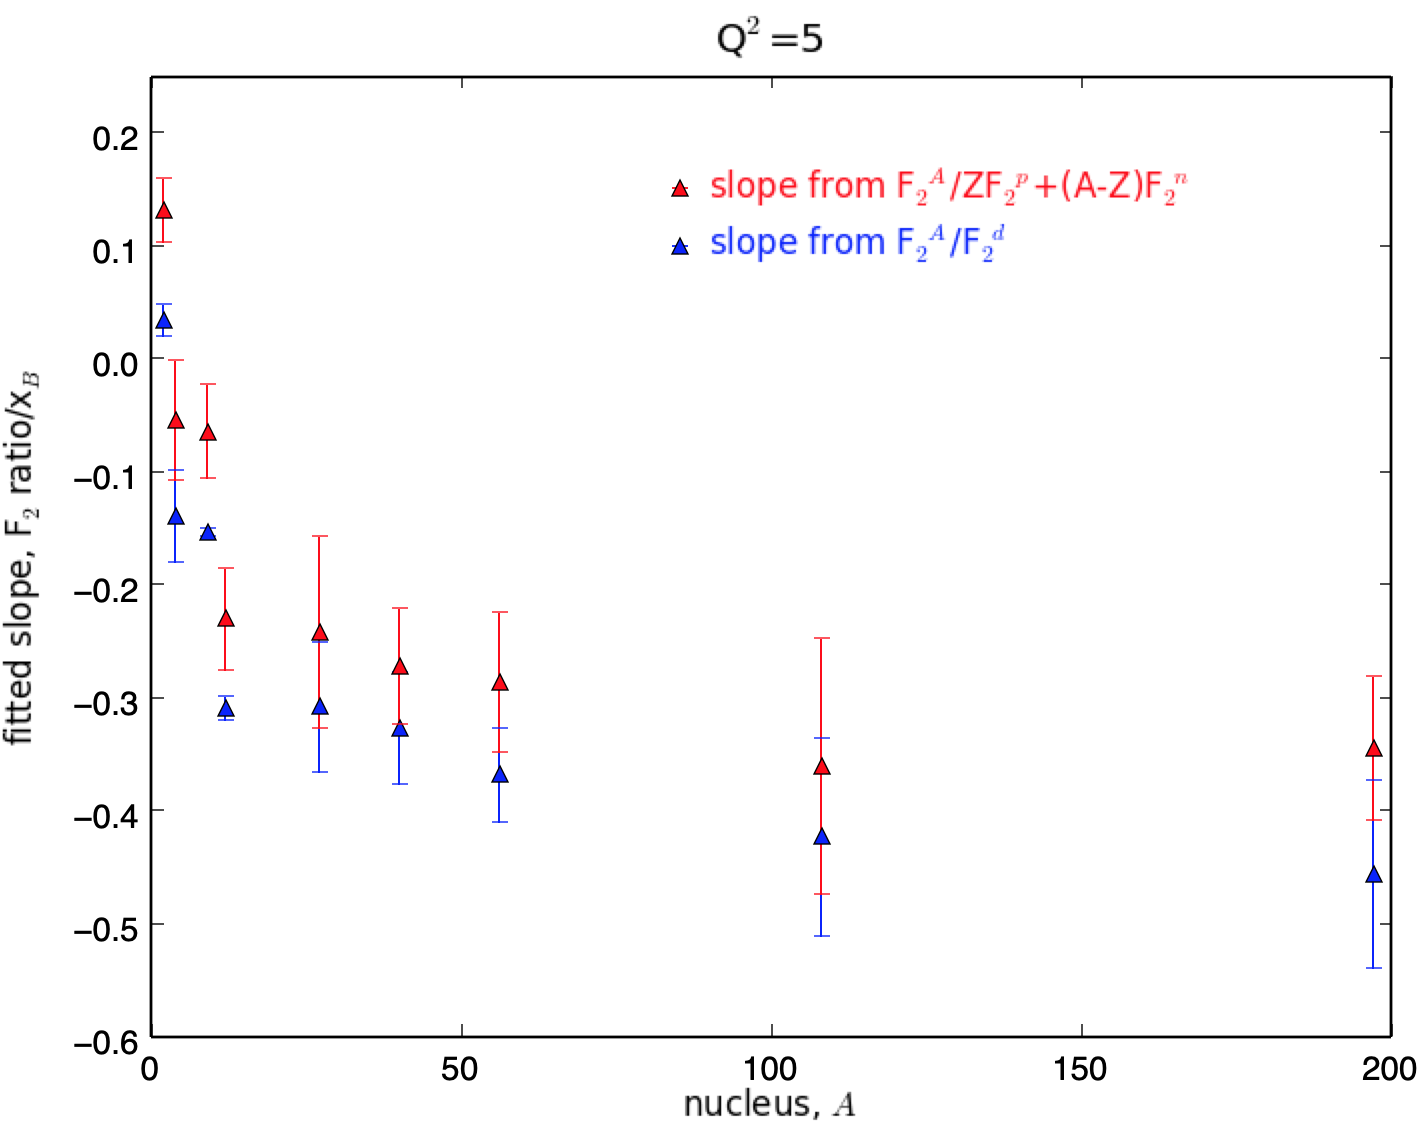
\includegraphics[width=\textwidth]{plots/plotsvA/Aslope_q5.png}
\end{minipage}\hfill\begin{minipage}{0.5\textwidth}
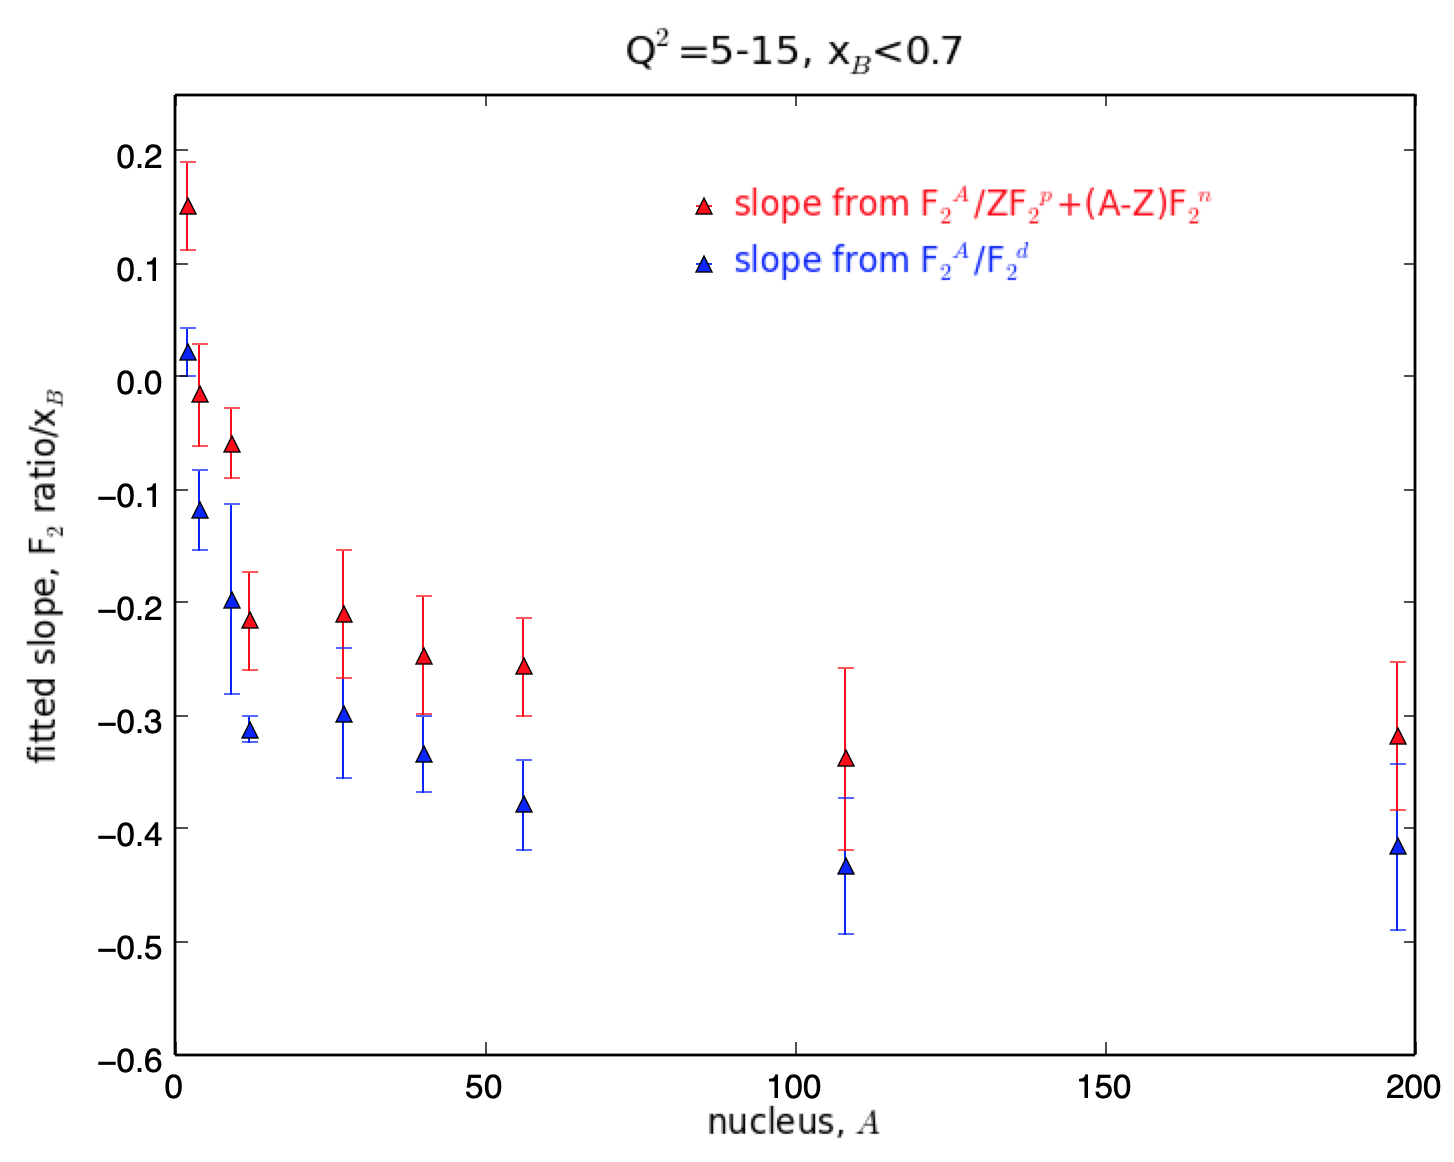
\includegraphics[width=\textwidth]{plots/plotsvA/Aslope_l7.png}
\end{minipage}\hfill\begin{minipage}{0.5\textwidth}
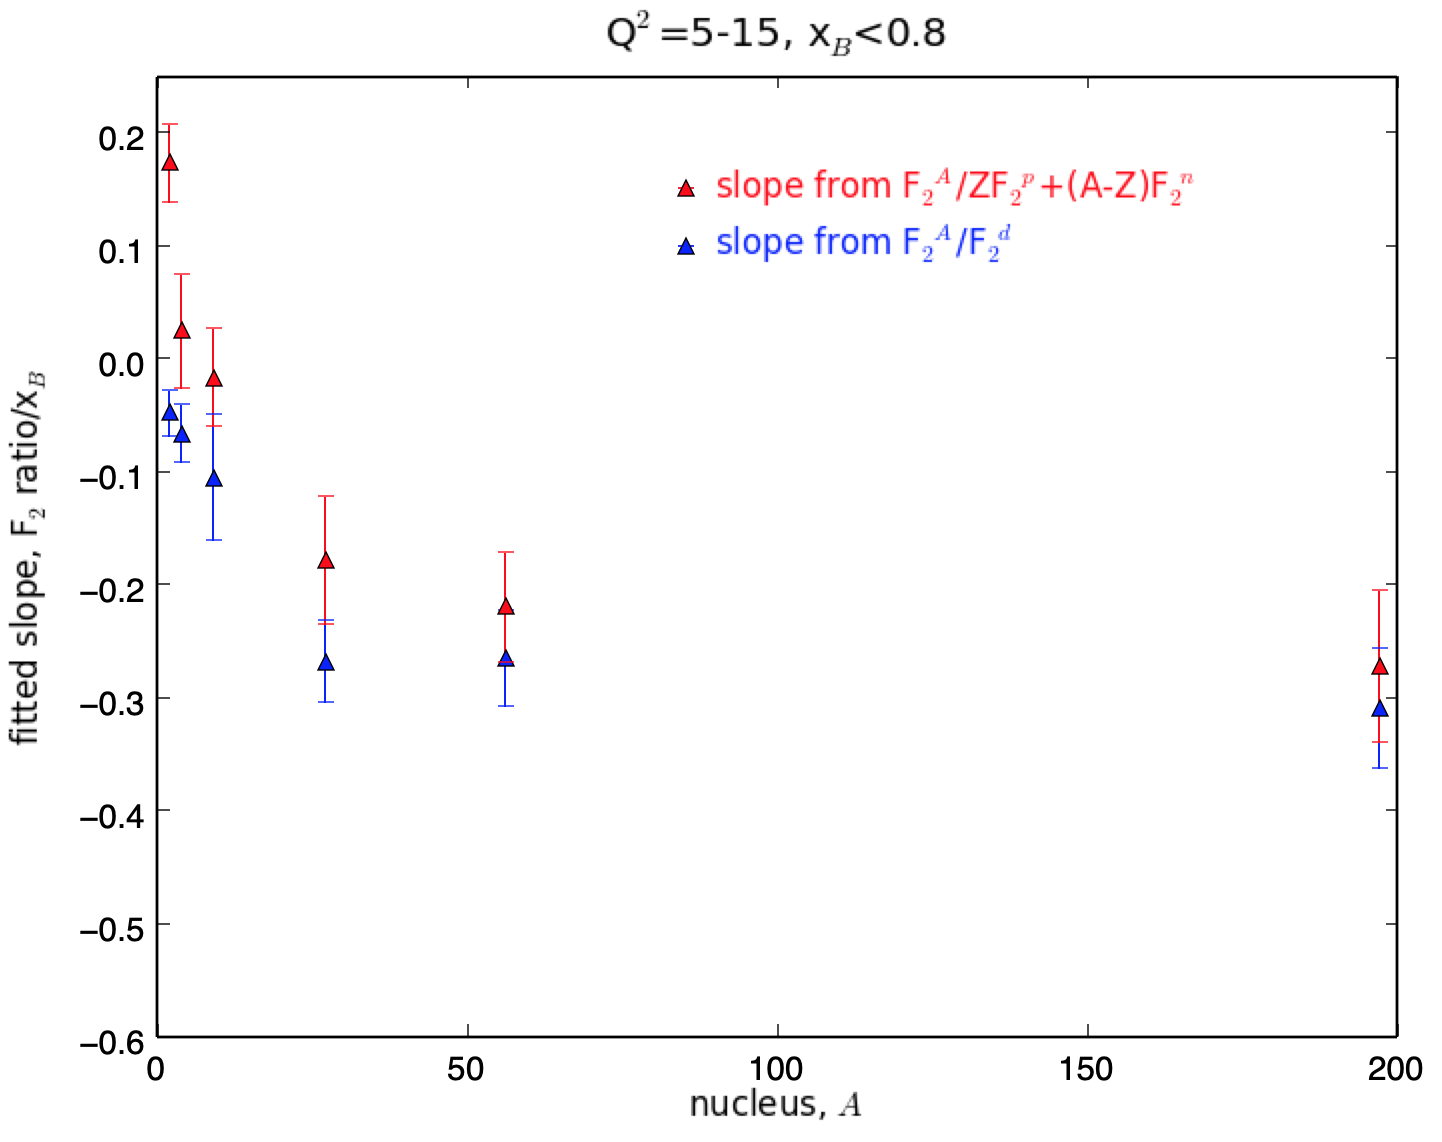
\includegraphics[width=\textwidth]{plots/plotsvA/Aslope_all.png}
\end{minipage}
  \caption[]{.}
  \label{fig:Aslope_summary}
\end{figure}   

\begin{figure}[H]
\begin{minipage}{0.5\textwidth}
 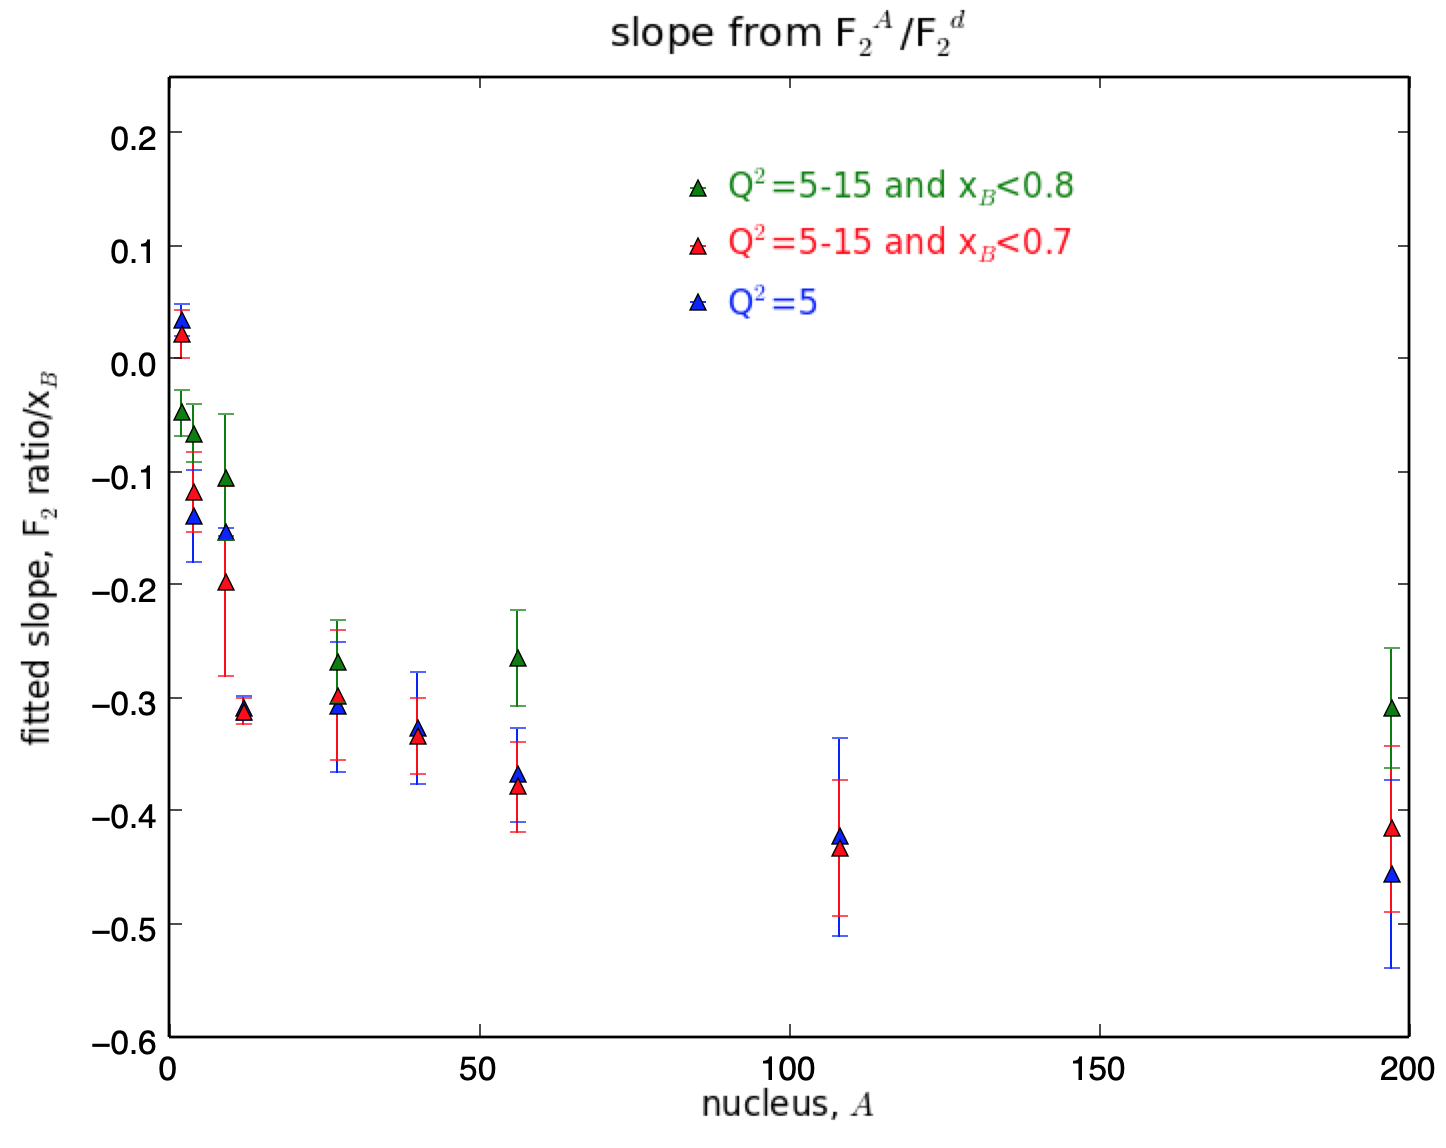
\includegraphics[width=\textwidth]{plots/plotsvA/Aslope_ad.png}
\end{minipage}\hfill\begin{minipage}{0.5\textwidth}
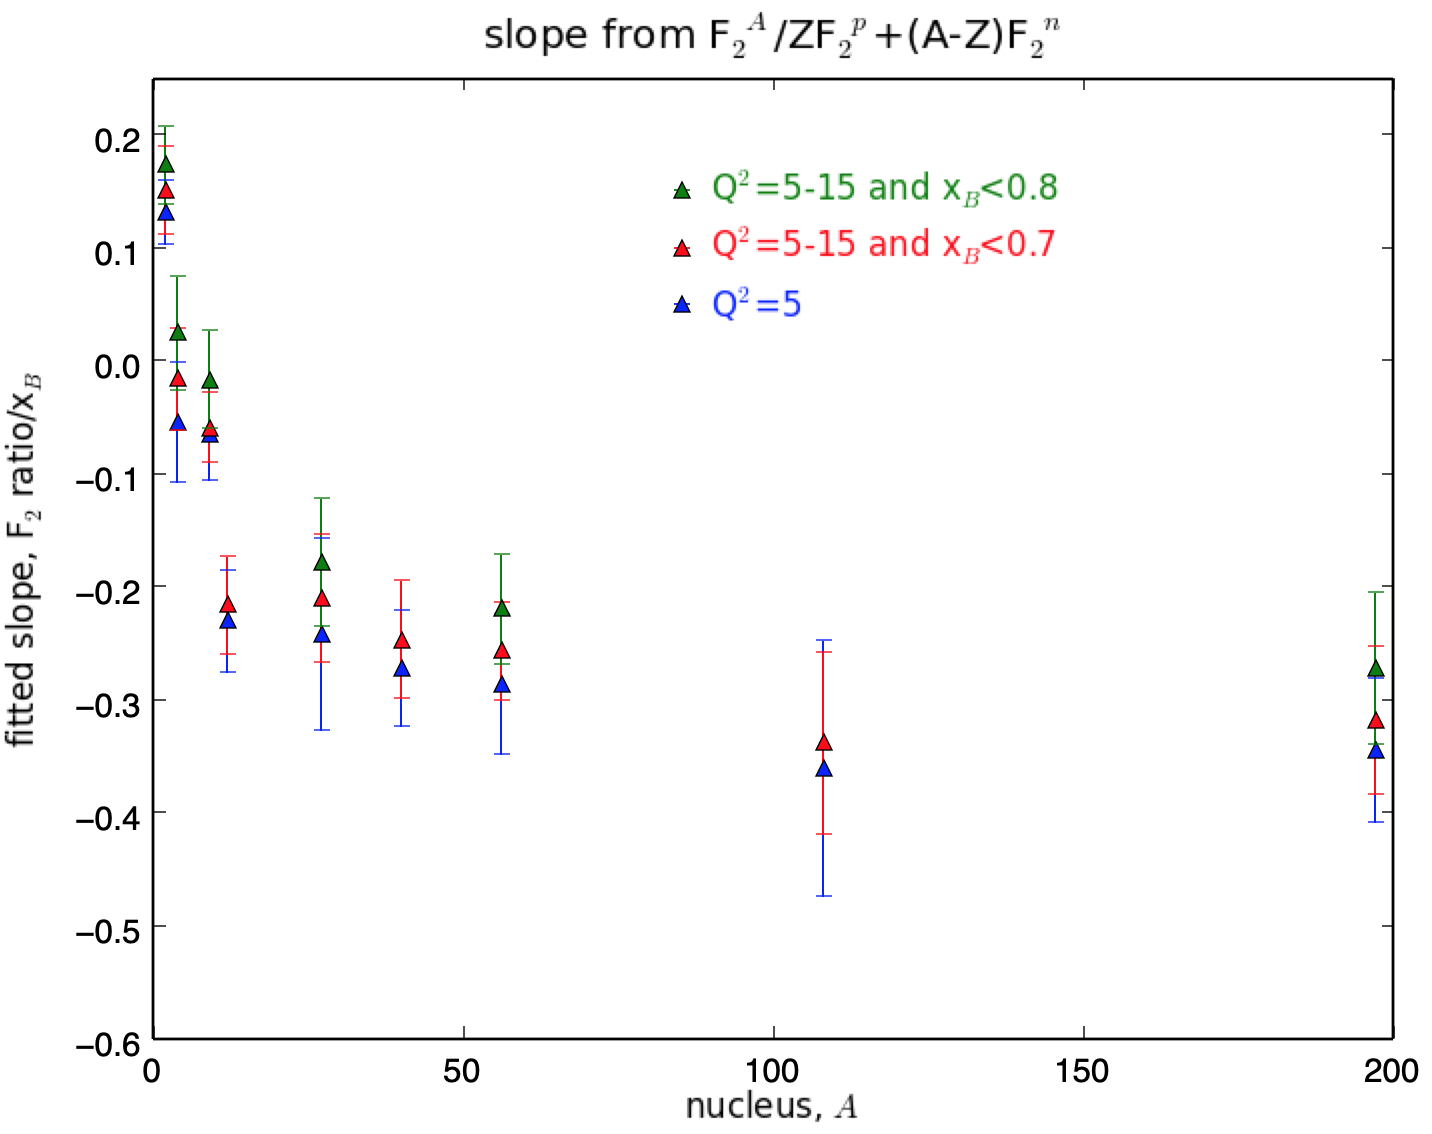
\includegraphics[width=\textwidth]{plots/plotsvA/Aslope_free.png}
\end{minipage}
  \caption[]{.}
  \label{fig:Aslope_compare}
\end{figure}   

\end{document}
